%%%%%%%%%%%%%%%%%%%%%%%%%%%%%%%%%%%%%%%%%
% Masters/Doctoral Thesis 
% LaTeX Template
% Version 2.5 (27/8/17)
%
% This template was downloaded from:
% http://www.LaTeXTemplates.com
%
% Version 2.x major modifications by:
% Vel (vel@latextemplates.com)
%
% This template is based on a template by:
% Steve Gunn (http://users.ecs.soton.ac.uk/srg/softwaretools/document/templates/)
% Sunil Patel (http://www.sunilpatel.co.uk/thesis-template/)
%
% Template license:
% CC BY-NC-SA 3.0 (http://creativecommons.org/licenses/by-nc-sa/3.0/)
%
%%%%%%%%%%%%%%%%%%%%%%%%%%%%%%%%%%%%%%%%%

%%%%%%%%%%%%%%%%%%%%%%%%%%%%%%%%%%%%%%%%%
% This thesis template is an adaptation of the template mentioned above. It has been created by Giovanni Spadaro and it is available on GitHub (https://github.com/Giovo17/thesis-template-unict-lm-data).
%%%%%%%%%%%%%%%%%%%%%%%%%%%%%%%%%%%%%%%%%

%----------------------------------------------------------------------------------------
%	PACKAGES AND OTHER DOCUMENT CONFIGURATIONS
%----------------------------------------------------------------------------------------

\documentclass[
11pt, % The default document font size, options: 10pt, 11pt, 12pt
%oneside, % Two side (alternating margins) for binding by default, uncomment to switch to one side
english, % ngerman for German
singlespacing, % Single line spacing, alternatives: onehalfspacing or doublespacing
%draft, % Uncomment to enable draft mode (no pictures, no links, overfull hboxes indicated)
%nolistspacing, % If the document is onehalfspacing or doublespacing, uncomment this to set spacing in lists to single
%liststotoc, % Uncomment to add the list of figures/tables/etc to the table of contents
%toctotoc, % Uncomment to add the main table of contents to the table of contents
%parskip, % Uncomment to add space between paragraphs
%nohyperref, % Uncomment to not load the hyperref package
headsepline, % Uncomment to get a line under the header
%chapterinoneline, % Uncomment to place the chapter title next to the number on one line
%consistentlayout, % Uncomment to change the layout of the declaration, abstract and acknowledgements pages to match the default layout
]{MastersDoctoralThesis} % The class file specifying the document structure

% These are the main packages you could use for your thesis. You can remove the unused ones.

\usepackage[utf8]{inputenc} % Required for inputting international characters
%\hyphenation{ма-те-ма-ти-ка вос-ста-нав-ли-вать}
\usepackage{amsmath}
\usepackage{algorithmic}
\usepackage{algorithm}
\usepackage{verbatim}
\usepackage{amsfonts}
\usepackage{siunitx}
\usepackage{subfloat}
\usepackage{changepage}
\usepackage{float}
\usepackage{subfig}
\usepackage{textcomp}
\usepackage{enumitem}
\usepackage{hyperref}
\usepackage{lmodern} % Use the Palatino font by default
\usepackage{eso-pic}
\usepackage{setspace}
\usepackage[nottoc]{tocbibind}
\usepackage{diagbox}
\usepackage{nicefrac}
\usepackage{breqn}
\usepackage[autostyle=true]{csquotes} % Required to generate language-dependent quotes in the bibliography

\usepackage{amsthm}

% O in alternativa style = authoryear
\usepackage[backend=bibtex,style=ieee,natbib=true]{biblatex} % Use the bibtex backend with the authoryear citation style (which resembles APA)

\addbibresource{thesisBibliography.bib} % The filename of the bibliography



% ------- This part defines some new commands, like Theorem, Lemma or the command used for the centering the first image

\theoremstyle{plain} 
\newtheorem{thm}{Theorem}[section] 
\newtheorem{cor}[thm]{Corollary} 
\newtheorem{lem}[thm]{Lemma} 
\newtheorem{prop}[thm]{Proposition} 

\theoremstyle{definition} 
\newtheorem{defn}{Definition}[chapter] 

\theoremstyle{remark} 
\newtheorem{obs}{Observation} 

\newcommand\alcentropagina[1]{\AddToShipoutPicture{%
		\AtPageCenter{\makebox(50,0){\includegraphics[width=1.2\textwidth]{#1}}}}}


%----------------------------------------------------------------------------------------
%	MARGIN SETTINGS
%----------------------------------------------------------------------------------------

\geometry{
	paper=a4paper, % Change to letterpaper for US letter
	inner=2.0cm, % Inner margin 
	outer=3.0cm, % Outer margin
	%bindingoffset=.5cm, % Binding offset
	top=1.5cm, % Top margin
	bottom=1.5cm, % Bottom margin
	%showframe, % Uncomment to show how the type block is set on the page
}

%----------------------------------------------------------------------------------------
%	THESIS INFORMATION
%----------------------------------------------------------------------------------------

\thesistitle{Оптимизация экономического портфеля с помощью методов машинного обучения} % Your thesis title, this is used in the title and abstract, print it elsewhere with \ttitle
\supervisor{д-р физ.-мат. наук, профессор А.В. \textsc{Леонидов}} % Your supervisor's name, this is used in the title page, print it elsewhere with \supname

%\cosupervisor{Dr. A B}  % Your cosupervisor's name, this is used in the title page, print it elsewhere with \cosupname

\examiner{} % Your examiner's name, this is not currently used anywhere in the template, print it elsewhere with \examname
%\degree{Data Science} % Your degree name, this is used in the title page and abstract, print it elsewhere with \degreename
\author{Mikhail Davydov} % Your name, this is used in the title page and abstract, print it elsewhere with \authorname
\addresses{} % Your address, this is not currently used anywhere in the template, print it elsewhere with \addressname

\subject{Компьютерные науки} % Your subject area, this is not currently used anywhere in the template, print it elsewhere with \subjectname
\keywords{} % Keywords for your thesis, this is not currently used anywhere in the template, print it elsewhere with \keywordnames
\university{\href{https://mipt.ru/}{Московский физико-технический институт}} % Your university's name and URL, this is used in the title page and abstract, print it elsewhere with \univname
\departmentb{\href{https://old.mipt.ru/education/chairs/dm/}{
Кафедра дискретной математики
}}
% Your department's name and URL, this is used in the title page and abstract, print it elsewhere with \deptname
\group{\href{http://researchgroup.university.com}{Research Group Name}} % Your research group's name and URL, this is not used in the title page, print it elsewhere with \groupname
\faculty{\href{https://old.mipt.ru/education/departments/fpmi/}{Факультет прикладной математики и информатики}} % Your faculty's name and URL, this is used in the title page and abstract, print it elsewhere with \facname

\AtBeginDocument{
\hypersetup{pdftitle=\ttitle} % Set the PDF's title to your title
\hypersetup{pdfauthor=\authorname} % Set the PDF's author to your name
\hypersetup{pdfkeywords=\keywordnames} % Set the PDF's keywords to your keywords
}

\begin{document}

\frontmatter % Use roman page numbering style (i, ii, iii, iv...) for the pre-content pages

%----------------------------------- FRONTESPIZIO GRANDE ----------------------
\newgeometry{
	paper=a4paper, % Change to letterpaper for US letter
	inner=3cm, % Inner margin
	outer=2.5cm, % Outer margin
	bindingoffset=.5cm, % Binding offset
	top=3.5cm, % Top margin
	bottom=1.5cm, % Bottom margin
}

%%%%%%%%%%%%%%%%%% PRIMA PAGINA %%%%%%%%%%%%%%%%%%

% Use roman page numbering style (i, ii, iii, iv...) for the pre-content pages

\pagestyle{plain} % Default to the plain heading style until the thesis style is called for the body content
\begin{titlepage}
	\begin{center}
		
		
		
\includegraphics[scale=0.15]{Figures/logos/mipt.eps} % University/department logo - uncomment to place it
            
		
		\vspace*{.06\textheight}  
		%{\color{red!50!black}{\scshape\LARGE \univname \par}\vspace{1.2cm}} % University name
		{\scshape\large \facname \par}\vspace{0.35cm} % Department 1 name
            {\scshape\large \deptbname \par}\vspace{0.35cm} % Department 1 name
            % {\scshape\large \deptcname \par}\vspace{1cm} % Department 1 name
		
		\textsc{\Large Степень бакалавра}\\[0.5cm] % Thesis type
		
		\HRule \\[2cm] % Horizontal line
		{\huge \bfseries \ttitle\par}\vspace{1cm} % Thesis title
		

		{БАКАЛАВРСКИЙ ДИПЛОМ}\vspace{1cm} % Thesis
		
		\begin{minipage}[t]{0.4\textwidth}
			\begin{flushleft} \large
				\emph{Автор}\\ 
				{Михаил Давыдов \\ Б05-024} % Author name - remove the \href bracket to remove the link
			\end{flushleft}
		\end{minipage}
		\begin{minipage}[t]{0.4\textwidth}
			\begin{flushright} \large
				\emph{Научный руководитель} \\
				{\supname} \\ % Supervisor name - remove the \href bracket to remove the link 
			\end{flushright}
		\end{minipage}\\[2cm]
		
		\vfill
		
		%\large \textit{A thesis submitted in fulfillment of the requirements\\ for the degree of \degreename}\\[0.3cm] % University requirement text
		%\textit{in the}\\[0.4cm]
		%\groupname\\\deptname\\[2cm] % Research group name and department name
		
		\vfill
		\HRule \\[1cm] % Horizontal line
		{\large Академический год 2023/2024 \\ 24 июня 2024}\\[4cm] % Date
		
		\vfill
	\end{center}
\end{titlepage}

\clearpage

%----------------------------------------------------------------------------------------
%	TITLE PAGE
%----------------------------------------------------------------------------------------

\begin{titlepage}
	\begin{center}
		% Logo al centro della paginaпочти
		\alcentropagina{Figures/logos/logounict_v2.pdf}
		\vspace{21cm}
		%
		% Autore
		\makeatletter
		\large\textrm{Михаил Давыдов}
		\makeatother
		\vspace{8.85cm}
		%
		% Titolo
		\begin{center}
			\makeatletter
			\singlespacing\Huge\textsc{\ttitle}
			\makeatother
		\end{center}%
		\vspace{0.4cm}
		%
		% Tipo di Tesi
		\makeatletter
		\large\textit{Бакалаврский диплом}
		\makeatother
		\vfill
		%
		\large МФТИ\\
		\vspace{1cm}
		%
		% Data Esame di Laurea
		\makeatletter
		\large\textrm{Июнь 2024} % Add month and year of your graduation
		\makeatother
	\end{center}
\end{titlepage}

\ClearShipoutPicture



\restoregeometry

\pagestyle{plain} % Default to the plain heading style until the thesis style is called for the body content

%----------------------------------------------------------------------------------------
%	QUOTATION PAGE
%----------------------------------------------------------------------------------------

% Remove this page if you do not want to add a quotation reference

% \vspace*{0.2\textheight}

% \noindent\enquote{\itshape What we know is a drop, what we don't know is an ocean.}\bigbreak

% \hfill Isaac Newton

%----------------------------------------------------------------------------------------
%	ABSTRACT PAGE
%----------------------------------------------------------------------------------------

\begin{abstract}
\addchaptertocentry{\abstractname} % Add the abstract to the table of contents
Задача о многоруких бандитах -- одна из базовых задач, встречающихся в обучении с подкреплением. Однако в большинстве случаев рассматривается очень простая версия этой задачи -- когда распределения всех рычагов есть гауссовские случайные величины, а функция полезности зависит только от матожидания этого распределения. Такой подход неприменим на практике, например, когда в качестве рычагов берутся активы, колебание стоимости которых ведет себя скорее как распределение Стьюдента, и в функцию полезности которого включается неприятие к риску.

В этой работе была рассмотрена эффективность алгоритмов для решения задачи о многоруких бандитах для распределений, отличных от нормального. В результате получено снижение эффективности стандартных алгоритмов для распределений Стьюдента с малым числом степеней свободы и низкую эффективность известных стратегий для распределения Коши. Были разработаны алгоритмы для нахождения точки на многомерном симплексе, максимизирующей функцию полезности с учетом неприятия к риску, а также адаптированы алгоритмы из обычной задачи о многоруких бандитах для задачи с учетом неприятия к риску. Была рассмотрена эффективность полученных алгоритмов. Получена высокая эффективность алгоритмов для распределений Стьюдента с большим числом степеней свободы $\nu$ и низкая эффективность для распределений Стьюдента с $\nu=2.1$.
\end{abstract}



%----------------------------------------------------------------------------------------
%	LIST OF CONTENTS/FIGURES/TABLES PAGES
%----------------------------------------------------------------------------------------

\tableofcontents % Prints the main table of contents

\listoffigures % Prints the list of figures

\listoftables % Prints the list of tables

\listofalgorithms % Prints the list of algorithms

%----------------------------------------------------------------------------------------
%	ABBREVIATIONS
%----------------------------------------------------------------------------------------

% \begin{abbreviations}{ll} % Include a list of abbreviations (a table of two columns)

% \textbf{LAH} & \textbf{L}ist \textbf{A}bbreviations \textbf{H}ere\\
% \textbf{WSF} & \textbf{W}hat (it) \textbf{S}tands \textbf{F}or\\

% \end{abbreviations}

%----------------------------------------------------------------------------------------
%	PHYSICAL CONSTANTS/OTHER DEFINITIONS
%----------------------------------------------------------------------------------------

% \begin{constants}{lr@{${}={}$}l} % The list of physical constants is a three column table

% The \SI{}{} command is provided by the siunitx package, see its documentation for instructions on how to use it

% Speed of Light & $c_{0}$ & \SI{2.99792458e8}{\meter\per\second} (exact)\\
%Constant Name & $Symbol$ & $Constant Value$ with units\\

% \end{constants}

%----------------------------------------------------------------------------------------
%----------------------------------------------------------------------------------------

\begin{symbols}{ll} % Include a list of Symbols (a three column table)

$t_{\nu}$ & Распределение Стьюдента с $\nu$ степенями свободы. В случае, когда $\nu > 2$, распределение домножено на $\sqrt{\frac{\nu - 2}{\nu}}$, чтобы дисперсия была равна 1 \\
$t_{\infty}$ & Стандатное нормальное распределение \\
$\Delta^n$ & Многомерный симплекс $= \{(p_1, ..., p_n): \sum_{i=1}^n p_i = 1 \land \forall i \hookrightarrow p_i \geq 0 \}$ \\

% \addlinespace % Gap to separate the Roman symbols from the Greek

\end{symbols}

%----------------------------------------------------------------------------------------
%	DEDICATION
%----------------------------------------------------------------------------------------

% Remove if you do not want to dedicate your work

% \dedicatory{For/Dedicated to/To my\ldots} 

%----------------------------------------------------------------------------------------
%	THESIS CONTENT - CHAPTERS
%----------------------------------------------------------------------------------------

\mainmatter % Begin numeric (1,2,3...) page numbering

\pagestyle{thesis} % Return the page headers back to the "thesis" style

% Include the chapters of the thesis as separate files from the Chapters folder
% Uncomment the lines as you write the chapters

% Chapter Template

\chapter{Введение} % Main chapter title

\label{Introduction} % Change X to a consecutive number; for referencing this chapter elsewhere, use \ref{ChapterX}

\newcommand{\tbf}[1]{\textbf{#1}}
\newcommand{\hook}{\hookrightarrow}
\newcommand{\bb}[1]{\mathbb{#1}}

%----------------------------------------------------------------------------------------
%	SECTION 1
%----------------------------------------------------------------------------------------

\section{Мотивировка}

\subsection{Описание проблем}
\label{sec:problem_description}

Инвесторы вкладывают свои деньги в акции, чтобы сохранить или приумножить свои богатства. Представим себе, что инвестор хочет вложить деньги в $n$ акций. Будем считать, что $i$-ая акция за определенный фиксированный промежуток времени увеличивается в своей стоимости на значение случайной величины $\xi_i$ , причем $\forall \, i, \, j, \: i \neq j \hook \xi_i \perp \xi_j$. Инвестору необходимо найти оптимальный вектор $\tbf{p} \in \Delta^n$, максимизирующий получаемую в среднем субъективную прибыль от активов за один промежуток времени, скажем, за день. Для максимизации прибыли инвесторы могут использовать модели для приближенного вычисления изменения стоимости акций \cite{bouchaudpotters}. Если инвестор не обладает информацией о стоимости активов (например, актив только появился, или до этого данные об активе были засекречены), то в качестве одной моделей можно использовать модель многоруких бандитов.

Классическая задача о многоруких бандитах звучит так: есть $n$ рычагов, каждый ход можно выбрать один из рычагов, и в ответ на выбор $i$-ого рычага игрок получает награду из распределения, связанного с $i$-ым рычагом \cite{suttonbarto}. Цель -- максимизировать среднюю награду $\bb{E} R_T$ спустя $T$ шагов, например, 1000. Оптимальной стратегией является нажатие на лучшие рычаги, то есть рычаги с наибольшим матожиданием (в случае, если нам неинтересны риски) или, если матожидания нет, с наибольшим значением по какой-то единой для всех рычагов метрике, например, по медиане. Проблема заключается в том, что изначально распределения наград для рычагов неизвестны, и их надо приблизить нажатиями на рычаги и получением выборки наград.

В таком случае задача инвестора -- последовательными изменениями своего экономического портфеля и  ``нажатиями на рычаги'' найти такое распределение денег по акциям, которое в среднем дает наибольший прирост стоимости портфеля. Для нахождения распределения денег можно использовать стандартные алгоритмы из задачи о многоруких бандитах.

В предложенной схеме есть несколько проблем:
\begin{enumerate}
    \item В качестве распределений рычагов (то есть распределений изменений активов в цене) чаще всего берется гауссовское распределение, в то время как в реальной жизни гораздо чаще наблюдаются степенные распределения с более тяжелыми хвостами.
    \item Кроме матожидания, инвесторы также заинтересованы в учете рисков при вкладывании денег в актив, поскольку портфель должен быть предсказуемым. Классическая постановка задачи о многоруких бандитах учитывает только матожидание (то есть среднюю награду) каждого рычага, совершенно не учитывая риски.
    \item В качестве распределений рычагов для решения задачи о многоруких бандитах берутся распределения из одного семейства, например, из семейства нормальных случайных величин. В реальном мире, естественно, изменения активов могут быть подчинены распределениям не из одного семейства.
\end{enumerate}

\subsection{Подход к решению проблем}

Для упрощения задачи в этой работе опущена треться проблема, то есть считается. что распределения берутся из одного семейства. Что касается остального, то здесь естьь способы их решения.

Для решения первой проблемы было решено проверить классические алгоритмы из задачи о многоруких бандитах, такие как $\epsilon$-greedy, Positive Initialisation, Upper-Confidence Bound (UCB), Gradient Bandits, для распределений Стьюдента с разными степенями свободы. Распределение Стьюдента было взято по нескольким причинам. Во-первых, его хвосты подчинены степенному распределению, что близко к реальному изменению цен активов. Во-вторых, изменение параметра числа степеней свободы $\nu$ задает меру хаотичности распределения: от отсутствия матожидания и почти полного хаоса при $\nu=1$, что соответствует распределению Коши, до упорядоченности при $\nu \to \infty$, что соответствует нормальному распределению.

Что касается второй проблемы, то необходимо задать функцию полезности, включающей риски и максимизацией которой будут заниматься алгоритмы. Мы возьмем версию функции полезности, основанной на дисперсии. Итак, есть $n$ рычагов, $i$-ый рычаг соответствует какому-то распределению со средним $m_i$ и дисперсией $\sigma_i^2$. Распределения изначально нам неизвестны. Каждый ход мы можем выбрать один из рычагов, при выборе $i$-го рычага мы получаем награду, сгенерированную из $i$-го распределения. После $t$-го шага у нас имеется вектор вероятностей $P_t = (p_1^t, ..., p_n^t)$, $\forall i \: p_i \geq 0$, и рычаг выбирается в соотвествии с этим вектором. Цель -- за $T$ шагов по получаемым наградам максимизировать $V = m_p - \lambda \cdot \sigma_p^2 = \sum_{i=1}^n p_i^T m_i - \lambda \sum_{i=1}^n (p_i^T)^2 \sigma_i^2$, то есть найти такой вектор $\textbf{p}^* \in \Delta^n$, что $\tbf{p}^* = \underset{\tbf{p} \in \Delta^n}{\arg \max} \sum_{i=1}^n p_i m_i - \lambda \sum_{i=1}^n p_i^2 \sigma_i^2$. Число $\lambda > 0$ называется степенью (коэффициентом) отвращения к риску (неприятия риска).

Почему функция полезности $V$ выглядит именно так? Будем считать, что вектор $\tbf{p}$ описывает собой доли денег, вкладываемых инвестором каждый шаг в каждый из активов. \cite{bouchaudpotters}. По-другому говоря, если инвестор решает за ход вложить $M$ денег в активы, то в $i$-ый актив будет вложено $p_i M$ денег. Для удобства положим $M=1$. Тогда матожиидание увеличения стоимости портфеля будет составлять $m_p = \sum_{i=1}^n p_i m_i$, а матожидание рисков будет равно дисперсии портфеля, то есть $\sigma_p^2 = \sum_{i=1}^n (p_i)^2 \sigma_i^2$. Таким образом, максимизация $V$ равносильна максимизации $m_p - \lambda \sigma_p^2$, то есть разности среднего увеличения портфеля и средних рисков портфеля, домноженных на степень неприятия к риску.

Для максимизации этой функции полезности $V$ были разработаны алгоритмы, находящие оптимальный вектор вероятностей $\tbf{p}$, максимизирующий $V$ при условии известных значений матожиданий и дисперсии. Далее описанные выше стратегии из обычной задачи о многоруких бандитах были адаптированы для задачи с учетом неприятия к риску, в их основу положен алгоритм нахождения оптимального вектора вероятностей. Наконец, все измененные стратегии были протестированы на распределениях Стьюдента с разным числом степеней свободы.

Дополнительно стоит отметить, что, хотя для $\nu > 2$ у распределения Стьюдента с $\nu$ степенями свободы есть дисперсия и, следовательно, определена функция полезности, при $\nu \to 2+$ могут начать происходить интересные явления. В работе проанализировано влияние этих явлений на эффективность максимизации $V$ и сделаны выводы о применимости оценки рисков с учетом дисперсии для использования в реальном мире.

\section{Обзор литературы}

Главная работа, в которой описываются основные алгоритмы для решения задачи о многоруких бандитах, является книга Ричарда Саттона и Эндрю Барто "Reinforcement Learning: An Introduction" \cite{bouchaudpotters}. Хотя описание алгоритмов снабжено многочисленными графиками и сравнениями эффективности алгоритмов, в их описании прослеживаются несколько описанных выше проблем. Во-первых, в качестве распределений для рычагов используются нормальные распределения и не рассматриваются никакие другие распределения, что является серьезным упущением. Во-вторых, поскольку в их цели не входило обширное исследование задачи о многруких бандитах, никак не был учтен риск от выбора того или иного рычага.

Другой работой, в которой исследуется вопрос максимизации функции полезности с учетом неприятия к риску, является портфельная теория Марковица, описанная, в частности, в \cite{bouchaudpotters}. В теории вычислено точное значение вектора $\tbf{p}$, а также помимо дисперсии рассмотрен другой подход к измерению риска - Value at Risk (VaR) \cite{varbouchaudpotters}. Однако при этом присутствует 2 недостатка:
\begin{enumerate}
    \item Изначально все матожидания и дисперсии считаются известными, что не всегда соответствует действительности.
    \item В оптимальном решении могут быть ШортЫ (то есть максимум функции полезности берется не по симплексу $\Delta^n$, а по всей гиперплоскости $\{(p_1, ..., p_n): \sum_{i=1}^n p_i = 1\}$). Инвесторы не всегда могут давать деньги в долг.
\end{enumerate}

Таким образом, хотя вышеперечисленные работы приводят исследования описанных в \ref{sec:problem_description} проблем, они все же обладают некоторыми недостатками, а, главное, рассматривают модели отдельно, не пытаясь объединить их в одную общую модель. Эта работа устраняет описанные проблемы, предлагая стратегии для их решения.

\section{Структура}

В главе \ref{Theory} этой работы сначала описываются стратегии для итеративного приближения оптимального решения, каждый шаг которых работает за $O(n^2)$. Затем описываются стохастические методы для нахождения оптимального вектора при условии известных матожиданий и дисперсий, основанные на градиентном подъеме. Далее предлагаются алгоритмы, работающие за $O(n \log n)$. Стандартные стратегии, такие как $\epsilon$-greedy, позитивная инициализация, UCB, Gradient bandits, изменены для оптимальной работы с учетом неприятия к риску. В основу этих стратегий положен самый удачный из алгоритмов за $O(n \log n)$. Кроме того, предложена новая стратегия, основанная на коррекции выборочной дисперсии. В главе \ref{ExperimentsClassic} проводятся экспермиенты для стандартных стратегий и различных распределений, полученные результаты визуализируются, приводится объяснение наблюдаемым явлениям, даются пргнозы по эффективности стратегий для задачи о многоруких бандитах с учетом неприятия к риску. Все стратегии сравниваются при различных гиперпараметрах. В главе \ref{ExperimentsAversion} проводятся эксперименты для разработанных во второй главе стратегий для задачи о могоруких бандитах с измененной функцией полезности, аналогично, результаты визуализируются и объясняются. Наконец, в пятой главе (ССЛЫКА!) делаются общие выводы об эффективности стратегий и о применимости в реальной жизни их и постановки задачи оптимизации портфеля, основанной на дисперсии. Кроме того, описываются дальнейшие направления развития теории.

Код, реализующий все алгоритмы, а также саму статью можно найти \href{https://github.com/davynchi/diploma/blob/main}{в репозитории} на Github.












\chapter{Теория} % Main chapter title

\label{Theory} % Change X to a consecutive number; for referencing this chapter elsewhere, use \ref{ChapterX}

\newcommand{\lrarr}{\lrarr}

%%%%%%%%%%%%%%%%%%%%%%%%%%%%%%%%%%%%%%%%%%%%%%%%%%%%%%%%%%%%%%%%%%%%%%%%%%%%%%%%%%%%%%%%%%%

В этой главе мы рассмотрим подходы для нахождения оптимального вектора вероятностей. Будут представлены аналоги greedy, $\epsilon$-greedy, стратегий с позитивной инициализацией, UCB, Gradient bandits, а также некоторые замечания по сэмплированию Томпсона.  

\section{Формализация задачи}

\subsection{Постановка задачи}

Итак, еще раз повторим задачу: имеется $n$ рычагов, $i$-ый рычаг соответствует какому-то распределению $\xi_i$ со средним $m_i$ и дисперсией $\sigma_i^2$. Распределения изначально неизвестны. Каждый ход мы можем выбрать один из рычагов, при выборе $i$-го рычага мы получаем награду, сгенерированную из $\xi_i$. После $t$-го шага у нас имеется вектор вероятностей $P_t = (p_1^t, ..., p_n^t)$, $\forall i \: p_i \geq 0$, и на $t+1$-ом шаге вероятность выбора $i$-го рычага равна $p_i^t$. Задача -- за $T$ шагов по получаемым наградам максимизировать $V = m_p - \lambda \cdot \sigma_p^2 = \sum_{i=1}^n p_i^T m_i - \lambda \sum_{i=1}^n (p_i^T)^2 \sigma_i^2$, где $\lambda > 0$. Максимизация достигается путем нахождения такого вектора вероятностей $\tbf{p}^*$, что $\tbf{p}^* = \underset{\tbf{p} \in \Delta^n}{\arg \max} \sum_{i=1}^n p_i m_i - \lambda \sum_{i=1}^n p_i^2 \sigma_i^2$. Далее всегда будем считать, что в первый ход рычаг выбирается случайно, то есть $\tbf{p}_1 = \left( \frac{1}{n}, ..., \frac{1}{n} \right)$. \\

В некоторых случаях у распределения нет дисперсии. Например, это верно для распределения Стьюдента $t_2$ с двумя степенями свободы. Если дисперсии нет у распределения $\zeta$, то считаем, что любое распределение $\xi_i \sim c_i \cdot \zeta$, и ставится задача максимизации $V = \sum_{i=1}^n p_i^T m_i - \lambda \sum_{i=1}^n (p_i^T)^2 c_i^2$, то есть в качестве меры риска берется ''растяжение'' $\xi_i$ относительного какого-то эталонного распределения $\zeta$.

\subsection{Обозначения}

Введем обозначения:
\begin{itemize}
    \item $R_t$ -- награда, полученная на $t$-ом шаге (то есть сразу после того момента, когда нажали на рычаг в $t$-ый раз).
    \item $A_t$ -- номер рычага, выбранный на $t$-ом шаге.
    \item $R_t(a) = R_t \cdot \bb{I}(A_t = a)$.
    \item $N_t(a) := \sum_{i=1}^{t-1} I(A_i = a)$ -- количество нажатий на рычаг $a$ на $t$-ом шаге (перед процедурой нажатия в $t$-ый раз). Соответственно, на нулевом шаге $\forall a \hook N_t(a) = 0$.
    \item $Q_t(a) := \frac{\sum_{i=1}^{t-1} R_i(a)}{N_t(a)}$ -- средняя награда рычага $a$ на шаге $t$. Можно считать, что обновление происходит так: если на шаге $t$ было выбрано действие $a$, то для всех остальных действий $b$ значение $Q_t(b)$ не меняется, а для действия $a$ $Q_t(a) = Q_t(a) + \frac{1}{N_{t}(a) + 1}(R_t - Q_t(a))$. Заметим, что $Q_t(a)$ является выборочным матожиданием рычага $a$ по всем полученным от его нажаатия наградам.
    % \item $\bar{R_t} := \frac{\sum_{i=1}^{t-1} R_i}{max(t-1,1)}$ -- средняя награда за все предыдущие шаги, или, как ее называют по-другому, baseline.
    \item $\overline{R_t^2(a)} = \frac{\sum_{i=1}^{t-1} R_i^2(a)}{N_t(a)}$ -- средняя квадратичная награда рычага $a$ на шаге $t$. Аналогично средней награде, можно считать, что каждый ход происходит обновление только одного значения.
    \item $S_t^2(a) = \frac{1}{N_t(a) - 1}\sum_{i=1}^{t-1}(R_i(a) - Q_t(a))^2 = \frac{N_t(a)}{N_t(a) - 1}(\overline{R_t^2(a)} - Q_t(a)^2)$ -- выборочная дисперсия. Если $N_t(a) \leq 1$, будем считать, что $S_t^2(a) = 0$.
\end{itemize}

\subsection{Подсчет матожидания и дисперсии}

Будем приближать матожидание и дисперсию рычагов с помощью выборочного матожидания и выборочной дисперсии соответственно. Заметим, что $\bb{E} \, Q_t(a) = m_a$, $\bb{E} \, S_t(a) = \sigma_a^2$ (за исключением холодного старта, то есть случая $N_t(a) \leq 1$), и такие приближения корректны. Кроме того:
\begin{itemize}
    \item Для невыбранных на $t$-ом шаге рычагов обновления выборочного матожидания и дисперсии не происходит.
    \item $Q_{t+1}(A_t) = Q_t(A_t) + \frac{1}{N_{t}(A_t) + 1}(R_t - Q_t(A_t))$, поэтому обновление выборочного матожидания происходит за $O(1)$.
    \item $\overline{R_{t+1}^2(A_t)} = \overline{R_t^2(A_t)} + \frac{1}{N_{t}(A_t) + 1}(R_t^2 - \overline{R_t^2(A_t)})$ -- подсчет тоже происходит за $O(1)$.
    \item Так как $S_t^2(a) = \frac{N_t(a)}{N_t(a) - 1}(\overline{R_t^2(a)} - Q_t(a)^2)$, а $\overline{R_t^2(a)}$ и $Q_t(a)^2$ пересчитываются за $O(1)$, то и $S_t^2(a)$ пересчитывается за $O(1)$.
\end{itemize}

\section{Жадные стратегии}

В классической задаче о многоруких бандитах под жадной стратегией подразумевался выбор каждый ход рычага с наибольшим выборочным матожиданием, то есть $A_t = \underset{a}{\arg \max} Q_t(a)$. Поскольку это самая простая стратегия, она страдает от проблемы холодного старта: представим себе 2 рычага, $m_1 > m_2 > 0$. Пусть на первом шаге был прожат второй рычаг. Поскольку $m_2 > 0$, то велика вероятность получения награды $R_1 > 0$, так что $0 = Q_2(1) < Q_2(2) = R_1$. Поэтому далее снова прожмется второй рычаг и так далее. Поскольку по ЗБЧ $Q_t(2) \to m_2 > 0$, то с высокой вероятностью $\forall t \hook Q_t(2) > 0$ (особенно если $m_2$ сильно больше нуля), и первый рычаг никогда не выберется, хотя он дает большее матожидание. 

\subsection{Итеративные жадные стратегии}

В отличие от обычной задачи о многоруких бандитах, в измененной версии для жадных стратегий вектор вероятностей выбора рычагов $\tbf{p}_t$ может быть не равен вектору $(0, ..., 1, 0, ..., 0)$. Каждый шаг будем менять вероятность выбора каждого рычага в соответствии с новой полученной наградой. ``Жадность'' будет выражаться в несколько другом смысле. Опишем сначала процесс изменения вероятностей для итеративных greedy-стратегий. Под итеративными стратегиями будем понимать стратегии, которые при заданных матожиданиях и дисперсиях сходятся к оптимальному вектору вероятностей за $k > 1$ проходов какого-то кода, но на каждом шаге производящих только один проход этого кода.

Пусть на $t$-ом шаге вектор вероятностей равен $\tbf{p}_t = (p_1^t,...,p_n^t)$. Будем на каждом шаге изменять вероятности так, чтобы максимально увеличить $V = Q_{t,p} - \lambda S_{t,p}^2$, где $Q_{t,p} = \sum_{i=1}^n p_i^t Q_t(i)$, $S_{t,p}^2 = \sum_{i=1}^n (p_i^t)^2 S_t(i)^2$. Можно рассмотреть 2 подхода.

\subsubsection{Изменение двух вероятностей}
\label{subsec:iterative_greedy_changing_two_probs}

Далее для облегчения обозначений будем вместо $p_t^i$ использовать $p_i$, а вместо $p_{t+1}^i$ -- $p_i^{new}$. \\
Каждый ход будем увеличивать одну из вероятностей $p_i$ на $\Delta p \geq 0$, а другую вероятность $p_j$ -- уменьшать на $\Delta p$. Сумма вероятностей не изменилась. Будем искать такие $i, \, j, \, \Delta p$, что $p_i^{new} \leq 1, p_j^{new} \geq 0$ и увеличение $V$ (обозначим за $\Delta V$) максимально. Заметим, что $p_i + \Delta p \leq 1 \lrarr \Delta p \leq 1 - p_i, \; p_j - \Delta p \geq 0 \lrarr \Delta p \leq p_j$ и $1 - p_j \geq p_i \lrarr p_i + p_j \leq 1$, поэтому условие $p_i^{new} \leq 1$ избыточно. После изменения соответствующих вероятностей получим:
\begin{multline}
    \Delta V =\left[ (p_i + \Delta p) Q_t(i) + (p_j - \Delta p) Q_t(j) - \lambda (p_i + \Delta p)^2 S_t^2(i) - \lambda (p_j - \Delta p) S_t^2(j) \right] - \left[  p_i Q_t(i) + p_j Q_t(j) - \lambda p_i^2 S_t^2(i) - \lambda p_j^2 S_t^2(j) \right] = \Delta p (Q_t(i) - Q_t(j)) - 2 \lambda \Delta p (p_i S_t^2(i) - p_j S_t^2(j)) - \lambda (\Delta p)^2 \left[ S_t^2(i) + S_t^2(j) \right] = \Delta p \left( [Q_t(i) - 2 \lambda p_i S_t^2(i)] - [Q_t(j) - 2 \lambda p_j S_t^2(j)]\right) - \lambda (\Delta p)^2 \left[ S_t^2(i) + S_t^2(j) \right] \overset{w_k := Q_t(k) - 2 \lambda p_k S_t^2(k)}{=} (w_i - w_j) \Delta p - \lambda \left[ S_t^2(i) + S_t^2(j) \right] (\Delta p)^2
    \label{eq:2}
\end{multline}
Если $\lambda > 0$, $S_t^2(i) \neq 0 \lor S_t^2(j) \neq 0$, то получили квадратный многочлен с отрицательным главным коэффициентом. Этот многочлен достигает максимума в точке $\Delta p = \frac{w_i - w_j}{2 \lambda (S_t^2(i) + S_t^2(j))}$ и этот максимум равен $\frac{(w_i - w_j)^2}{4 \lambda \left[ S_t^2(i) + S_t^2(j) \right]}$. Заметим, что $w_i - w_j = - (w_j - w_i)$ и поэтому при перестановке $i$ и $j$ значение $\Delta p$ изменится на противоположное, поэтому $p_i + \Delta p$ и $p_j - \Delta p$ не изменятся, как и ограничения на них. Для удобства будем рассматривать только такие пары $(i,j)$, что $w_i - w_j \geq 0$. Так как отрезок $\left[0, \min \left(p_j, \frac{w_i - w_j}{2 \lambda \left[ S_t^2(i) + S_t^2(j) \right]} \right) \right]$ находится левее точки максимума, то при заданных ограничениях максимум $\Delta V$ достигается при $\Delta p = \min \left( p_j, \frac{w_i - w_j}{2 \lambda \left[ S_t^2(i) + S_t^2(j) \right]} \right)$. Посчитав $\Delta V$ для всех пар $(i,j)$ с $w_i - w_j > 0$, сможем найти оптимальные $i, \, j, \, \Delta V$.

Если $\lambda = 0$, то задача сводится к обычной задаче о многоруких бандитах. Если же $S_t^2(i) = S_t^2(j) = 0$, то многочлен равен $\Delta p (Q_t(i) - Q_t(j)$. Опять, можно считать, что $Q_t(i) \geq Q_t(j)$, так как иначе знак $\Delta p$ меняется на противоположный, и максимальное значение $\Delta V$ не меняется. Тогда оптимальное $\Delta p = p_j$ и $\max \Delta V = (Q_t(i) - Q_t(j)) p_j$. Тот факт, что $S_t^2(i) = 0$, означает, что или количество нажатий на $i$-ый рычаг $ \leq 1$, или $i$-ый рычаг всегда выдаёт одно и то же значение (то есть рычаг безрисковый), или распределение $i$-го рычага дискретное, но все полученные до этого значения при нажатии на $i$-ый рычаг были одинаковыми. В случае, когда оба рычага безрисковые, и эти 2 рычага были выбраны для изменения вероятностей, $p_j^{new} = 0$, то есть безрисковый рычаг с меньшим значением больше не будет выбираться, как и в оптимальном векторе вероятностей. 

Обратим внимание на проблему холодного старта: после первого шага, когда был выбран только один $i$-ый рычаг, может оказаться, что полученная награда $> 0$, в то время как выборочные дисперсии всех рычагов и выборочное матожидание всех других рычагов нулевое. В таком случае наибольшая разница $\Delta V$ будет достигаться при увеличении вероятности выбранного рычага на $\frac{1}{n}$ и уменьшении вероятности какого-то другого рычага $j$ до $p_j^{new} = 0$. То есть $j$-ый рычаг больше не будет выбран, хотя он может быть ``лучше'' $i$-го рычага. Если же полученная награда $< 0$, то тогда обнулится вероятность выбора $i$-го рычага, хотя нам могло просто не повезти с наградой. О том, как справляться с этой проблемой, мы поговорим позднее.

Кроме того, алгоритм каждый шаг меняет всего 2 вероятности, что медленно, а сам шаг совершается за $O(n^2)$ (в то время как greedy-стратегия в оюычной задаче о многоруких бандитах -- за $O(n)$).
    
\iffalse
\subsubsection{Изменение всех вероятностей}

В качестве альтернативы можно пытаться за один шаг менять сразу все вероятности. Одна из вероятностей будет изменяться в одну сторону, а остальные -- в другую. Отдельно будем рассматривать случаи с увеличением этой единственной вероятности и с ее уменьшением.
    
    Пусть на $t$-ом шаге $\phi_t$ рычагов с ненулевыми вероятностями выбора, то есть $|\{i: p_t^i \neq 0\}| = \phi_t$ и пусть $K_t := \{i: p_t^i \neq 0\}$. Будем каждый ход увеличивать одну из вероятностей $p_i$ на $\Delta p_{\uparrow}$, а все остальные ненулевые вероятности -- уменьшать на $\frac{\Delta p_{\uparrow}}{\phi_{t,i}}$, где $\phi_{t,i} := \phi_t - \mathbb{I}_{p_i \neq 0}$. Сумма вероятностей не изменилась. Будем искать такие $i, \, \Delta p_{\uparrow}$, что $\forall j \hook 1 \geq p_j^{new} \geq 0$ и значение $\Delta V_{\uparrow}$ максимально. Если $\phi_{t,i} = 0$, то $p_i = 1$, и $\Delta p_{\uparrow} = \Delta V_{\uparrow} = 0$. Иначе после изменения соответствующих вероятностей получим:
    \begin{dmath}
        \Delta V_{\uparrow} = \Delta p_{\uparrow} \left(Q_t(i) - \frac{\sum_{\substack{j \in K_t \\ j \neq i}} Q_t(j)}{\phi_{t,i}} \right) - 2\lambda \Delta p_{\uparrow} \left( p_i S_t^2(i) - \frac{\sum_{\substack{j \in K_t \\ j \neq i}} p_j S_t^2(j)}{\phi_{t,i}} \right) - \lambda (\Delta p_{\uparrow})^2 \left( S_t^2(i) + \frac{\sum_{\substack{j \in K_t \\ j \neq i}} S_t^2(j)}{\phi_{t,i}^2} \right) = \Delta p_{\uparrow} \left( w_i - \frac{\sum_{\substack{j \in K_t \\ j \neq i}} w_j}{\phi_{t,i}} \right) - \lambda (\Delta p_{\uparrow})^2 \left( S_t^2(i) + \frac{\sum_{\substack{j \in K_t \\ j \neq i}} S_t^2(j)}{\phi_{t,i}^2} \right) = \Delta p_{\uparrow} \frac{\sum_{\substack{j \in K_t \\ j \neq i}} (w_i - w_j)}{\phi_{t,i}} - \lambda (\Delta p_{\uparrow})^2 \frac{\sum_{\substack{j \in K_t \\ j \neq i}} (\phi_{t,i} S_t^2(i) + S_t^2(j))}{\phi_{t,i}^2}
        \label{eq:3}
    \end{dmath}
    Если $\lambda \neq 0$ и $\exists j \in K_t \cup \{i\} \hookrightarrow S_t^2(j) \neq 0$, то получаем квадратный многочлен, максимум которого в точке
    $$\Delta p_{\uparrow} = \frac{\phi_{t,i} \sum_{\substack{j \in K_t \\ j \neq i}} (w_i - w_j)}{2\lambda \sum_{\substack{j \in K_t \\ j \neq i}} ( \phi_{t,i} S_t^2(i) + S_t^2(j) )}$$
    и в этой точке достигается значение
    $$ \Delta V_{\uparrow} = \frac{\left( \sum_{\substack{j \in K_t \\ j \neq i}} (w_i - w_j) \right)^2}{4\lambda \sum_{\substack{j \in K_t \\ j \neq i}} ( \phi_{t,i} S_t^2(i) + S_t^2(j) )}
    $$
    Здесь уже может быть $\Delta p_{\uparrow} < 0$. Если $\Delta p_{\uparrow} \geq 0$, то налагаются дополнительные ограничения $p_i^{new} \leq 1 \lrarr \Delta p_{\uparrow} \leq 1 - p_i$ и $\forall j \in K_t \setminus \{i\} \hookrightarrow p_j^{new} \geq 0 \lrarr \Delta p_{\uparrow} \leq \phi_{t,i} p_j$. Если же $\Delta p_{\uparrow} < 0$, то налагаются ограничения $p_i^{new} \geq 0 \lrarr \Delta p_{\uparrow} \geq -p_i$ и $\forall j \in K_t \setminus \{i\} \hookrightarrow p_j^{new} \leq 1 \lrarr \Delta p_{\uparrow} \geq \phi_{t,i} (p_j - 1)$. Итоговое $\Delta p_{\uparrow}$ берется как минимум (при $\Delta p_{\uparrow} \geq 0$) или как максимум (при $\Delta p_{\uparrow} < 0$) от аргмаксимума функции и ограничений.

     Если $\lambda = 0$, то задача сводится к обычной задаче о многоруких бандитах. Если же $\forall j \in K_t \cup \{i\} \hookrightarrow S_t^2(j) = 0$ (то есть безрисковые рычаги или $N_t(i) \leq 1$), то уравнение линейно или всегда равно 0 и достигает максимума в минимуме (если коээфициент $\geq 0$) или максимуме (если $\leq 0$) из ограничений.

     Аналогично, можно пытаться уменьшить одну вероятность $p_i$ на $\Delta p_{\downarrow}$, а все остальные, не равные 1 (пусть таких $\psi_{t,i}$) -- увеличить на $\frac{\Delta p_{\downarrow}}{\psi_{t,i}}$. Пусть $K_t = \{j: j \land p_j \neq 1 \}$. Проводя аналогичные вычисления, получим формулы:
     $$
     \Delta p_{\downarrow} = \frac{-\psi_{t,i} \sum_{\substack{j \in K_t \\ j \neq i}} (w_i - w_j)}{2\lambda \sum_{\substack{j \in K_t \\ j \neq i}} ( \psi_{t,i} S_t^2(i) + S_t^2(j) )}, \; \Delta V_{\downarrow} = \frac{\left( \sum_{\substack{j \in K_t \\ j \neq i}} (w_i - w_j) \right)^2}{4\lambda \sum_{\substack{j \in K_t \\ j \neq i}} ( \psi_{t,i} S_t^2(i) + S_t^2(j) )}
     $$
     На $\Delta p_{\downarrow}$ накладываются аналогичные ограничения, аналогично в случае, когда многочлен линейный. Аналогично вычисляется оптимальное $\Delta p$.

     Сравнивая все $\Delta V_{\uparrow}$ и $\Delta V_{\downarrow}$, найдем оптимальные $i, \, \Delta_p$ и тип измененния ($\uparrow$ или $\downarrow$).

     Нам нужно проверить 2 различных варианта для каждого рычага. Каждая проверка проходит за $O(n)$ (проверка на равенство 0 или 1, вычисление $\Delta_p$ и наложение не более $n$ ограничений), поэтому шаг алгоритма работает за $O(n^2)$. При этом, так как в этом методе мы изменяем сразу все вероятности, а не две, то он сходится быстрее, чем второй метод~\autoref{subsec:iterative_greedy_changing_two_probs}. Однако этот алгоритм гораздо сильнее страдает от проблемы холодного старта: если после первого шага при нажатии $i$-го рычага мы получили награду, большую 0, то наибольшее изменение $\Delta V$ будет достигаться для тройки $(i, \uparrow, \frac{n-1}{n})$, и вся вероятность сконцентрируется в $p_i$. Если затем всегда будет $Q_t(i) - \lambda S_t^2(i) > 0$, что вполне реально, то алгоритм всегда будет нажимать на $i$-ый рычаг, в то время как могут быть рычаги с большим матожиданием или меньшей дисперсией, на которые никогда не нажмут.

\subsubsection{Градиентный подъем}
Теперь опишем метод градиентного подъема. На каждом шаге $t$ рассмотрим функцию $Q_{t,p} - \lambda S_{t,p}^2 = \sum_{i=1}^n p_i Q_t(i) - \lambda \left( \sum_{i=1}^n p_i^2 S_t^2(i)\right)$. Заметим, что множество
     $$
     Q =
        \begin{cases}
           0 \leq p_1 \leq 1 \\
            ... \\
            0 \leq p_{n} \leq 1 \\
            p_1 + ... + p_n = 1
        \end{cases}
        \label{eq:4}
     $$
     есть $n$-мерный симплекс, а, значит, $Q$ выпукло и замкнуто. Далее, $V$ вогнута на $\mathbb{R}^n$, так как
     $$
     \frac{\partial V}{\partial p_i} = Q_t(i) - 2\lambda p_i S_t^2(i), \;
     \frac{\partial^2 V}{\partial p_i^2} = -2\lambda S_t^2(i), \;
     \frac{\partial^2 V}{\partial p_j \partial p_i} = 0 \; (j \neq i)
     $$
    и гессиан $V$ равен
    $$
    -2\lambda
    \begin{pmatrix}
        S_t^2(1)        &          &        &                  \\
                        & S_t^2(2) &        & \text{\huge{0}}  \\
        \text{\huge{0}} &          & \ddots &                  \\
                        &          &        & S_t^2(n)
    \end{pmatrix}
    \preceq 0
    $$
    и, кроме того, $V$ имеет липшицев градиент с параметром $2\lambda \sqrt{\underset{i}{\max}(S_t^2(i))}$, так как 
    \begin{multline}
        \sqrt{\frac{\| \nabla V (p) - \nabla V (q) \|_2^2}{\| p - q \|_2^2}} = \sqrt{\frac{4\lambda^2 \sum_{i=1}^n S_t^2(i) (p_i - q_i)^2}{\sum_{i=1}^n (p_i - q_i)^2}} \leq \\ \leq \sqrt{\frac{4\lambda^2 \underset{i}{\max}(S_t^2(i)) \sum_{i=1}^n (p_i - q_i)^2}{\sum_{i=1}^n (p_i - q_i)^2}} = 2\lambda \sqrt{\underset{i}{\max}(S_t^2(i))}
    \end{multline}
    Тогда метод градиентного отображения для функции $V' = -V$ сойдется к глобальному минимуму на $Q$, а, значит, для функции $V$ этот метод сойдется к глобальному максимуму на $Q$ \cite{nesterov_convergence}. В качестве альтернативы градиентному методу можно использовать проекцию градиента на симплекс \cite{simplex_projection}, вычисление которого происходит за $O(n)$, или Cauchy-Simplex метод \cite{cauchy_simplex}, тоже сходящийся к глобальному максимуму и требующий на каждом шаге $O(1)$ вычислений (однако серьезный минус заключается в очень медленной скорости сходимости $\| x^T - x^*\| \leq \frac{\log n}{T}$).

    Базовый алгоритм будет состоять в следующем: на каждом шаге $t$ выбираем рычаг согласно вероятностям $P_t$, обновляем выборочные дисперсии и матожидания, после чего с помощью градиентного подъема находим глобальный максимум $P_{t+1} = (p_{t+1}^1, ..., p_{t+1}^n)$ на $Q$, после чего повторяем алгоритм для $P_{t+1}$. Если обозначить $u$-ое значение метода градиентного подъема в ходе проведения алгоритма на шаге $t$ за $P_t^u$, а оптимальный вектор вероятностей на шаге $t$ за $P_t^*$, то тогда каждый шаг алгоритма работает за не более чем $O(k_t^{\Delta})$, где $k_t^{\Delta} = \underset{P \in Q}{\max} \min \{u: \| P_t^u - P_t^* \| \leq \Delta\}$ для заданной погрешности $\Delta$, так что шаг алгоритма может работать очень долго.

    Кроме того, никуда не делась проблема холодного старта: аналогично второму алгоритму, после первого шага все вероятности, кроме одной $p_t^i$, могут занулиться, и далее при $Q_t(i) - S_t^2(i) > 0$ вектор вероятностей не изменится.

    Изложенный выше алгоритм чем-то похож на Generalized Policy Iteration: процессом градиентного подъема можно считать policy evaluation, а нажатием рычага согласно вероятностям -- policy improvement \cite{suttonbarto_policy_iteration}. Однако здесь evaluation происходит одновременно еще и по матожиданию с дисперсией, и эти процессы друг с другом конфликтуют, что приводит к медленному или даже неверному приближению к ответу.

В заключение этого параграфа стоит заметить, что для обычной задачи о многоруком бандите все три алгоритма работают как обычные greedy-алгоритмы. Более того, все три алгоритма, как и стандартный greedy-алгоритм, страдают от проблемы холодного старта. Эти алгоритмы не единственны, для приближения вероятностей можно использовать метод Ньютона, метод штрафных функций, а также вместо одной или всех вероятностей пытаться за один ход изменять $k$ вероятностей, где $k = const$.

\subsubsection{Быстрый greedy алгоритм}
Есть алгоритм, находящий за $O(n \log n)$ распределение вероятностей, максимизирующее $Q_{t,p} - \lambda S_{t,p}^2$. Далее для удобства вместо $Q_{t,p}$ будем писать $m_p$ и вместо $S_{t,p}^2$ будем писать $\sigma_p^2$. Тогда:
\begin{enumerate}
    \item Пусть $i,j \in \{1, ..., n\}, \; i \neq j$. До этого мы рассматривали функцию $V(p_1, ..., p_n) = m_p - \lambda \sigma_p^2$. Рассмотрим функцию
    \begin{dmath}
        V(p_1, ..., p_n, \alpha) = p_1 m_1 + ... + (p_i + \alpha) m_i + ... + (p_j - \alpha) m_j + ... + p_n m_n - \lambda (p_1^2 \sigma_1^2 + ... + (p_i + \alpha)^2 \sigma_i^2 + ... + (p_j - \alpha)^2 \sigma_j^2 + ... + p_n^2 \sigma_n^2)
    \end{dmath}
    То есть $V(p_1, ..., p_n, \alpha) = V(p_1, ..., p_i + \alpha, ..., p_j - \alpha, ..., p_n)$. Возьмем точку $P^* \in Q$ (см. \ref{eq:4}), в которой достигается максимум $V$ на $Q$. Предположим, что $p_i^* \neq 1$ и $p_j^* \neq 0$. Тогда $\exists \delta > 0: \: \forall \alpha: \: 0 \leq \alpha < \delta \hookrightarrow P^*(\alpha) = (p_1^*, ..., p_i^* + \alpha, ..., p_j^* - \alpha, ..., p_n^*) \in Q$, и потому функция $V(p_1, ..., p_n, \alpha)$, определенная при $P \in Q, 0 \leq \alpha \leq \delta$, дифференцируема в точке $(P^*, 0)$ причем:
    \begin{dmath}
        \frac{\partial V(p_1, ..., p_n, \alpha)}{\partial \alpha}\bigg|_{P = P^*, \, \alpha = 0} = \left( (m_i - 2\lambda p_i^* \sigma_i^2 - \alpha \lambda \sigma_i^2) + (-m_j + 2\lambda p_j^* \sigma_j^2 - \alpha \lambda \sigma_j^2) \right) \bigg|_{\alpha = 0}  = (m_i - 2 \lambda p_i^* \sigma_i^2) - (m_j - 2 \lambda p_j^* \sigma_j^2) = w_i(p_i^*) - w_j(p_j^*) 
    \end{dmath}
    Если $\frac{\partial V}{\partial \alpha}\bigg|_{P = P^*, \, \alpha = 0} > 0$, то ввиду непрерывности $V(\alpha)$ существует $0 < \alpha < \delta: \: V(\alpha) > V(0) \land P(\alpha) \in Q$. Тогда максимум $V$ на $Q$ достигается не в $P^*$. Противоречие! $\Rightarrow \frac{\partial V}{\partial \alpha}\bigg|_{\alpha = 0} \leq 0 \Rightarrow w_i(p_i^*) \leq w_j(p_j^*)$.
    \item \label{itm:2} Пусть в точке оптиммума $P^*$ верно, что $p_i^* \in (0,1) \land p_j^* \in (0,1)$. Тогда, подставив в предыдущий пункт сначала пару $(i,j)$, а затем $(j,i)$, получим $w_i(p_i^*) \leq w_j(p_j^*) \land w_j(p_j^*) \leq w_i(p_i^*)$, то есть $w_i(p_i^*) = w_j(p_j^*)$. Аналогично, если $p_i^* = 0 \land p_j^* \neq 0$ или $p_j^* = 1 \land p_i^* > 0$ получим $w_i(p_i^*) \leq w_j(p_j^*)$. Заметим, что если есть $i$ с $p_i = 1$, то $\forall j \neq i \hookrightarrow p_j = 0$. Тогда, если $P^*$ -- точка оптимума на $Q$, то $\forall \, i,j: \: i \neq j \hookrightarrow w_i(p_i^*) = w_j(p_j^*) = w$ и $\forall \, i,j: \: p_i^* = 0, p_j^* \neq 0 \hookrightarrow w_i(p_i^*) \leq w_j(p_j^*)$, причем $\forall i \hookrightarrow w_i = m_i \lrarr p_i = 0$ \label{eq:5}.
    \item \label{itm:3} Итак, мы получили необходимое условие для точки оптимума. Является ли оно достаточным? Да, этого условия достаточно. Действительно, заметим, что $\frac{\partial V}{\partial p_i}\Bigg|_{P=P^*} = w_i(p_i^*)$. Кроме того, как мы уже показали, $Q$ выпукло и замкнуто, а $V$ нерперывно диффернцируема и вогнута на $\mathbb{R}^n$, и $-V$ выпукла на $\mathbb{R}^n$. Тогда по теореме об эквивалентном условии локального минимума на выпуклом замкнутом множестве \cite{nesterov_2_2_5} $P^*$ является минимумом функции $-V$ на $Q$ тогда и только тогда, когда $\forall P \in Q \hookrightarrow \left\langle (-V)'(P^*), \: P - P^* \right\rangle \geq 0 \Rightarrow$ $P^*$ является максимумом на $Q$ тогда и только тогда, когда
    \[
        \forall P \in Q \hookrightarrow \left\langle V'(P^*), \: P - P^* \right\rangle \leq 0
    \]
    Подставим $V'$ и $P^*$:
    \begin{dmath}
        \left\langle V'(P^*), \: P - P^* \right\rangle = \sum_{i=1}^n (m_i - 2\lambda p_i^* \sigma_i^2) (p_i - p_i^*) = \left( w \sum_{i: p_i^* \neq 0} p_i \right) \: + \left( \sum_{j: p_j^* = 0} m_j p_j \right) \: - \left( w \sum_{i: p_i^* \neq 0} p_i^* \right) \: - \left( \sum_{j: p_j^* = 0} m_j p_j^* \right) = w \left(1 - \sum_{j: p_j^* = 0} p_j \right) \:  + \left( \sum_{j: p_j^* = 0} m_j p_j \right) - w - 0 = \sum_{j: p_j^* = 0} (m_j - w) p_j \overset{(*)}{\leq} 0
    \end{dmath}
    Последнее неравенство $(*)$ верно, поскольку $\forall i,j: \: p_i = 0 \land p_j > 0 \hookrightarrow m_i = w_i \leq w_j = w$.

    Итак, неравенство выполнено, значит, в \ref{eq:5} описано эквивалентное условие глобального максимума на $Q$. Теперь перед описанием самого алгоритма осталось отметить пару деталей.
    \item \label{itm:4} Пусть $m_i < m_j$. Тогда не может быть такого, что $p_i^* \neq 0 \land p_j^* = 0$. Действительно, если бы это было так, то $w_i(p_i^*) = m_i - 2 \lambda p_i^* \sigma_i^2 \leq m_i < m_j = w_j(p_j^*)$, то есть $\exists i,j: \: p_j^* = 0 \land p_i^* \neq 0 \land w_i(p_i^*) <  w_j(p_j^*)$, то есть $P^*$ не является точкой оптимума. Противоречие! $\Rightarrow p_i^* = 0 \lor p_j^* \neq 0$. Кроме того, если $m_i = m_j$, то $p_i^* \neq 0 \land p_j^* = 0$ возможно только в том случае, когда $\sigma_i^2 = 0$, то есть $i$-ый рычаг безрисоквый. Поэтому, если упорядочить все $m_i$ по возрастанию и сопоставить каждому $m_i$ свой $p_i^*$, то все нулевые вероятности будут находиться ``не правее'' ненулевых вероятностей, причем в какой-то точке могут находиться одновременно ненулевые и нулевые вероятности только в том случае, когда неулевым вероятностям соответствуют безрисковые рычаги.
    \item\label{itm:5} Если $\forall i \sigma_i^2 > 0$ и $\exists i,\, j: \: m_i \neq m_j$, то существует метод нахождения $P^* = \underset{P}{\arg \max} (m_p - \lambda \sigma_p^2)$ на гиперплоскости $p_1 + ... + p_n = 1$, и для $P^*$ в таком случае верно, что 
    $$p_i^* = \frac{m_i}{2\lambda \sigma_i^2} + \frac{1 - \Sigma_1}{\Sigma_0} \cdot \frac{1}{2 \lambda \sigma_i^2}$$
    где 
    $$\Sigma_0 = \sum_{i=1}^n \frac{1}{2 \lambda \sigma_i^2}, \; \Sigma_1 = \sum_{i=1}^n \frac{m_i}{2 \lambda \sigma_i^2}$$ 
    Если $m_1 = m_2 = ... = m_n = m$, то для решения $P^*$ верно, что $p_i^* = \frac{1}{2\sigma_i^2 \Sigma_0}$ (док-во вкратце: фиксируем $m_p = m$, с помощью лагранжиана находим решение вида $p_i^* = \frac{\xi m + \xi'}{2\sigma_i^2}$, через ограничения находим зависимость $\xi$ и $\xi'$ от $m$, подставляем вероятности в $V$ при фиксированном $m_p = m$, получаем квадратное уравнение от $m$ с отрицательным главным коэф-ом, находим оптимальное $m$, подставляем сначала в $\xi$ и $\xi'$, а потом в $p_i^*$). Если же $\exists i: \: \sigma_i^2 = 0$, то есть существует безрисковый рычаг, то возьмем среди этих рычагов рычаг с наибольшим матожиданием $m_0$. Заметим, что $\exists P^*: \: \forall i \hookrightarrow (m_i \leq m_0 \Rightarrow p_i^* = 0)$, так как можно ``перекинуть'' все такие вероятности в безрисковый рычаг, не уменьшив $V$. Если не существует рычага с матожиданием, большим $m_0$, то оптимальным решением будет всегда нажимать на рычаг с $m_0$, в противном случае существует метод нахождения $P^* = \underset{P}{\arg \max} (m_p - \lambda \sigma_p^2)$ на гиперплоскости $p_1 + ... + p_n = 1$, и $p_i^* = \frac{m_i - m_0}{2 \lambda \sigma_i^2} \cdot \left(1 + m_0 \frac{\Sigma_1'}{\Sigma_2'} \right)$, где $\Sigma_k' = \sum_{i=1}^n \frac{(m_i - m_0)^k}{2 \sigma_i^2}$ и $i \neq 0$. То есть общее решение на гиперплоскости $p_1 + ... + p_n = 1$ существует. Также заметим, что оба алгоритма работают за $O(n)$ и что если в решении на этой гиперплоскости $\exists i: \: p_i \leq 0$, то в оптимальном решении на $Q$ существует $i$ с $p_i^* = 0$ ввиду вогнутости $V$.
    \item Теперь алгоритм описывается крайне просто:
    \begin{enumerate}
        \item Сортируем все $m_i$ по убыванию, в случае равенства по возрастанию $\sigma_i^2$. Работает за $O(n \log n)$.
        \item С начала массива ищем безрисковый рычаг с наибольшим матожиданием. Если нашли (это первый рычаг с $\sigma_i^2 = 0$), то отбрасываем все рычаги правее найденного $\left(O(n) \right)$. 
        \item Если отбросили все рычаги, кроме безрисокового, то вероятность выбора безрискового рычага равна 1, заканчиваем работу $\left( O(1) \right)$.
        \item Иначе проходимся бинпоиском по оставшемуся массиву и находим самое левое $i=I$ такое, что в оптимальном решении с рычагами $\{1, ..., i\}$ есть $j$ с $p_j^* \leq 0$. Оптимальный вектор вероятностей находится с помощтю формул из предыдущего пункта. Каждый шаг бинпоиска работает за $O(n)$, всего шагов $O(\log n)$, поэтому бинпоиск отработает за $O(n \log n)$.
        \item Возвращаем $(p_1^*, ..., p_{I-1}^*)$ для алгоритма от рычагов $\{1, ..., I-1\}$. Отрабатывает за $O(n)$.
    \end{enumerate}
    Во-первых, заметим, что итоговый алгоритм работает за $O(n \log n)$. Во-вторых, уже после отбрасывания рычагов, не может быть такого, что оптимальный вектор вероятностей для рычагов $\{1,...,k\}$ выдает $P_k^*$, в котором $\exists i: \: p_i^* = 0$, а оптимальный вектор вероятностей для рычагов $\{1, ..., l\}, \: k < l$ выдает $P_l^*$, в котором $\forall i \hookrightarrow p_i^* \neq 0$. Действительно, пусть для $k$ вектор вероятностей $(p_1, ..., p_{k-1}, 0)$ ($p_k = 0$, так как есть хотя бы одна нулевая вероятность и по \ref{itm:4}), а для $l$ вектор вероятностей $(q_1, ..., q_l)$, . Тогда по \ref{itm:2}: $\forall i \leq k - 1 \hookrightarrow m_i - 2 \lambda p_i \sigma_i^2 \geq m_k$ и $\forall i \leq k - 1 \hookrightarrow m_i - 2 \lambda q_i \sigma_i^2 = m_k - 2 \lambda q_k \sigma_k^2$. Так как мы рассматриваем этап после отбрасывания рычагов и $l > k$, то $\sigma_k^2 > 0$. Тогда $m_i - 2 \lambda q_i \sigma_i^2 = m_k - 2 \lambda q_k \sigma_k^2 < m_k \leq m_i - 2 \lambda p_i \sigma_i^2 \Rightarrow p_i < q_i \Rightarrow \sum_{i=1}^{k-1} p_i = 1 < \sum_{i=1}^{k-1} q_i$. Противоречие! $\Rightarrow$ если $k < l$, то либо среди $p_i$ нет нулей, либо среди $q_i$ есть нули. Тогда, если $A_k = \{1, ..., k\}$, то индексы $A_k$ для которых в оптимальном решении нет нулевых вероятностей, образуют отрезок $\overline{1, I - 1}$, и оптимальное решение обрзовано одним из этих $I - 1$ решений.

    Но заметим, что $(p_1, ..., p_k) = (p_1, ..., p_{k}, 0))$, поэтому для любого решения для $k$ рычагов с $V = V_k$ и решения для $k+1$ рычагов с $V = V_{k+1}$ верно, что $V_k \leq V_{k+1}$. Тогда решение для первых $I - 1$ рычагов -- оптимальное.

    \item Можно пойти дальше и сделать алгоритм еще быстрее, а именно, шаги (d) и (e) можно произвести за $O(n)$. Для этого воспользуемся альтернативной формулировкой оптимума, данной в пунктах \ref{itm:2} и \ref{itm:3}: достаточно найти такое распределение вероятностей $P=(p_1,...,p_n)$, что выполнено равенство \ref{eq:5}. Пусть мы отсортировали все рычаги и отбросили все, что хуже наилучшего безрискового. Посколку решение для \ref{eq:5} дает глобальный максимум на $Q$, то достаточно найти такое $t$, что $\forall i$ либо $m_i \leq t \land p_i = 0$, либо $m_i > t \land w_i = t \lrarr p_i = \frac{m_i - t}{2\lambda \sigma_i^2}$ и $\sum_{i=1}^n p_i = \sum_{i=1}^n p_i(t) = 1$. Для каждого $t$ однозначно определен набор тех $i$, для которых вероятности ненулевые, а именно такие $i$, что $m_i > t$. Кроме того, заметим, что при уменьшении $t$ сумма вероятностей увеличивается, а при $t = m_{(j)}$ (то есть $j$-ая порядковая статистика) верно, что 
    $$\sum_{i=1}^n p_i(m_{(j)}) = \sum_{i=j+1}^n \frac{m_{(i)} - m_{(j)}}{2 \lambda \sigma_{(i)}^2} = \sum_{i=j+1}^n \frac{m_{(i)}}{2 \lambda \sigma_{(i)}^2} \: - m_{(j)} \sum_{i=j+1}^n \frac{1}{2 \lambda \sigma_{(i)}^2} $$
    Если обозначить $\sum_{i=j+1}^n \frac{m_{(i)}}{2 \lambda \sigma_{(i)}^2} := \Sigma_1(j+1)$, а $\sum_{i=j+1}^n \frac{1}{2 \lambda \sigma_{(i)}^2} := \Sigma_0(j+1)$, то 
    $$\label{eq:fast}
        \sum_{i=1}^n p_i(m_{(j)}) = \Sigma_1(j+1) - m_{(j)} \Sigma_0(j+1)
    $$
    причем $\Sigma_1(n+1) = \Sigma_0(n+1) = 0$ и $$\Sigma_1(i) = \Sigma_1(i+1) + \frac{m_{(i)}}{2\lambda \sigma_{(i)}^2}, \: \Sigma_0(i) = \Sigma_0(i+1) + \frac{1}{2\lambda \sigma_{(i)}^2}$$
    Ввиду увеличения суммы вероятностей оптимальное $t$ либо лежит на полуинтервале \\ $(m_{(i)}, m_{(i+1)}]$ и $\sum_{j=1}^n p_j (m_{(i+1)}) \leq 1 < \sum_{j=1}^n p_j (m_{(i)})$, либо лежит на луче $(-\infty, m_{(1)})$ и $\sum_{j=1}^n p_j (m_{i+1}) \leq 1$. Во всех случаях мы можем вычислить $p_i$ по формулам из пункта \ref{itm:5}, учитывая только те $i$, для которых $m_{(i)} \geq t$, то есть все $m_{(i)}$ от конца интервала, где находится $t$, и до $m_{(n)}$. Итоговый алгоритм:
    \begin{enumerate}
        \item Сортируем все $m_i$ по убыванию, в случае равенства по возрастанию $\sigma_i^2$. Работает за $O(n \log n)$.
        \item С начала массива ищем безрисковый рычаг с наибольшим матожиданием. Если нашли (это первый рычаг с $\sigma_i^2 = 0$), то отбрасываем все рычаги правее найденного $\left(O(n) \right)$. 
        \item Если отбросили все рычаги, кроме безрисокового, то вероятность выбора безрискового рычага равна 1, заканчиваем работу $\left( O(1) \right)$.
        \item Иначе считаем $\Sigma_1(n+1) = \Sigma_0(n+1) = 0$, проходимся слева направо по $m_{(i)}$, пересчитывая за $O(1)$ $\Sigma_1(i+1)$ и $\Sigma_0(i+1)$, вычисляя за $O(1)$ по формуле \ref{eq:fast} сумму вероятностей. Находим первое такое $i$, что $\sum_{i=1}^n p_i(m_{(i+1)}) \leq 1$ и $\sum_{i=1}^n p_i(m_{(i+1)}) > 1$ $\left( O(n) \right)$.
        \item Если такое $i$ нашлось, то $p_j$ для $j \geq i + 1$ вычисляются по формулам из пункта \ref{itm:5} а для $j \leq i \hookrightarrow p_j = 0$. Если же не нашлось, то у всех рычагов ненулевые вероятности, и, аналогично, по формулам из пункта \ref{itm:5} вычисляются все $p_i$ $\left( O(n) \right)$.
    \end{enumerate}

    Алгоритм работает за $O(n \log n)$, но при этом быстрее, чем прошлый, так как часть после сортировки работает за $O(n)$, а не за $O(n \log n)$. Интересно заметить, что мы ищем пераое такое $t$, что $\sum_{j=i+1}^n \frac{m_{(j)} - t}{2\lambda \sigma_{(j)}^2} = 1 \lrarr t = \frac{\Sigma_1(i+1) - 1}{\Sigma_0(i+1)}$, а это похоже на формулы из статьи ``Projection onto a simplex''.
\end{enumerate}

Вообще стоит указать, что нам не так важна максимизация $V = m_p - \lambda \sigma_p^2$. Скорее, нам важна величина $\frac{\partial V}{\partial p_i}\Bigg|_{p_i = p_i^*} = w_i(p_i^*)$. Мы хотим найти такое распределение вероятностей, что 
\[
    \forall i,j \hookrightarrow (p_i^* = 0 \land p_j^* \neq 0 \Rightarrow w_i(p_i^*) \leq w_j(p_j^*))
\]
и что 
\[
    \forall i,j \hookrightarrow (p_i^* \neq 0 \land p_j^* \neq 0 \Rightarrow w_i(p_i^*) = w_j(p_j^*))
\]
Более того, в оригинальной задаче о многоруких бандитах требуется максимизировать $V = m_p$, что равносильно нахождению такого вектора вероятностей $(p_1^*, ..., p_n^*)$, что 
\[
    \forall i,j \hookrightarrow \left(p_i^* = 0 \land p_j^* \neq 0 \Rightarrow \frac{\partial V}{\partial p_i}\Bigg|_{p_i = p_i^*} = m_i \leq m_j = \frac{\partial V}{\partial p_j}\Bigg|_{p_j = p_j^*} \right)
\]
и что 
\[
    \forall i,j \hookrightarrow \left(p_i^* \neq 0 \land p_j^* \neq 0 \Rightarrow \frac{\partial V}{\partial p_i}\Bigg|_{p_i = p_i^*} = m_i = m_j = \frac{\partial V}{\partial p_j}\Bigg|_{p_j = p_j^*} \right)
\]
(см. \ref{itm:3})

\subsubsection{Альтернативный подход к изменению вероятностей} \label{subsubsec:iterative_greedy_changing_two_probs}

Но также можно рассмотреть совсем другой подход: На $t$-ом шаге будем считать, что $p_t^i = \frac{N_t(i)}{t-1}$, таким образом, вероятности формируются в зависимости от того, насколько часто выбирали рычаг. Далее посчитать $V_i = Q_t(i) - 2 \lambda p_i S_t^2(i)$ для каждого $i$ и взять рычаг для нажатия, исходя из максимума $V_i$. По сути, нам необходимо найти такое распределение вероятностей, что для ненулевых ыероятностей $w_i = w_j$, а все остальные $w_k$ не больше. Та же проблема холодного старта, но дополнительно на дальних шагах сложно изменить вероятности. Возможно, стоит отдавать большее ``предпочтение'' последним выборам рычагов (их вес больше веса других вероятностей). Или считать нажатия рычагов только в определенном окне (тогда снизится точность).

\subsection{\(\epsilon\)-greedy стратегии}

\subsubsection{Для градиентного подъема}

\begin{enumerate}
    \item На каждом шаге делать лишь $k$ итераций градиентного подъема (или даже одну итерацию) -- value iteration.
    \item После нахождения оптимума смещаться на случайный вектор, уменьшающийся по модулю со временем.
\end{enumerate}

\subsubsection{Для итеративных методов}
\begin{enumerate}
    \item Для первого метода брать $\Delta p_{final} = \min (\frac{p_i}{2}, \Delta p)$. То есть не смещаться сразу к краю. Аналогично для второго метода.
\end{enumerate}

\subsubsection{Для всех}
\begin{enumerate}
    \item С вероятностью $1-\epsilon$ выбирать согласно $P_t$, а с вероятностью $\epsilon$ -- случайно. $\epsilon$-greedy, по сути. Похоже на off-policy.
    \item Сначала прожать на каждый рычаг определенное число раз, чтобы иметь приближения $m_i$ и $\sigma_i^2$. В крайних случаях -- нажать по разу или по 2 раза (чтобы посчитать дисперсию).
    \item Можно использовать $\epsilon$-greedy стратегии с уменьшающимся $\epsilon$, а именно:
    \begin{enumerate}
        \item На $t$-ом шаге $\epsilon_t = \frac{1}{t}$ \cite{srank}
        \item VDBE: см. рис. \ref{fig:VDBE_epsilon}:
        \begin{figure}
            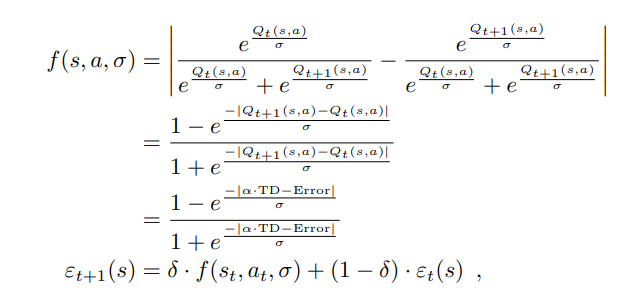
\includegraphics[width=0.8\linewidth]{theory/VDBE_epsilon.png}
            \caption{\label{fig:VDBE_epsilon} На $s$ можно не обращать внимания, $a$ -- выбранное на $t$-ом шаге действие, $\sigma$ -- температура: чем выше, тем ближе распределение к равномерному, чем меньше, тем ближе к жадному \cite{tolic_VDBE}}
        \end{figure}
        \item Epsilon-BMC. Пока не разобрался.
    \end{enumerate}
    В \href{https://en.wikipedia.org/wiki/Multi-armed_bandit}{Википедии} также описаны эти стратегии
    \item Если знаем, какому семейству распределений принадлежат рычаги, то можно для матожиданий и дисперсии в первых двух алгоритмах использовать границы (например) $95\%$-го доверительного интервала.
\end{enumerate}

\subsection{Optimistic initialization}
Можно инициализировать начальные значения всех рычагов большим положительным числом, как и в обычной оптимистичной инициализации. Изменять матожидание можно как среднее арифметическое, так и скользящим окном: $Q_{t+1}(a) = Q_t(a) + \alpha (R_t - Q_t(a))$.

Аналогично с $\overline{R_{t+1}^2(a)}$: $\overline{R_{t+1}^2(a)} = \overline{R_{t}^2(a)} + \alpha (R_t^2 - \overline{R_{t}^2(a)})$.

Выборочная дисперсия изменяется по формуле \ref{eq:1}. Но думаю, что оптимистичная инициализация с const step-size будет работать плохо, как и в обычной задаче о многоруких бандитах.

\subsection{UCB}
Можно ввести UCB для приближения, которое строится, исходя из выбранных ранее рычагов (\ref{subsubsec:iterative_greedy_changing_two_probs}). То есть, аналогично классическому UCB, $A_t = \underset{a}{\arg \max} \left( Q_t(a) - 2 \lambda p_a S_t^2(a) + c \sqrt{\frac{\ln t}{N_t(a)}} \right)$, где $p_a = \frac{N_t(a)}{t-1}$.

Можно еще пытаться что-то проделать с софтмаксом ($H_t(a)$ зависит от $Q_t(a), \, S_t^2(a), \, t, \, N_t(a)$, и $p_a = \frac{e^{H_t(a)}}{\sum_{i=1}^n e^{H_t(i)}}$). Но вот здесь уже меньше уверенности, что сработает.

\subsection{Gradient bandits}

Проводя аналогичные вычисления, что и в параграфе из книги ``Reinforcement Learning: An Inrtroduction'' \cite{suttonbarto_gradient_bandits}, получаем:
\[
    H_{t+1}(a) = H_t(a) + \alpha \frac{\partial \mathbb{E}(Q_{t,p} - \lambda S_{t,p}^2)}{\partial H_t(a)}
\]
\begin{dmath}
    \frac{\partial \mathbb{E}(m_{\pi} - \lambda \sigma_{\pi}^2)}{\partial H_t(a)} = \sum_{x} \left( m_x - 2 \lambda \pi_t(x) \sigma_x^2 \right) \frac{\partial \pi_t(x)}{\partial H_t(a)} = \mathbb{E} \left( \frac{m_{A_t}}{\pi_t(A_t)} - 2 \lambda \sigma_{A_t}^2 - B_t \right) \frac{\partial \pi_t(A_t)}{\partial H_t(a)} = \mathbb{E} \left( m_{A_t} - 2 \lambda \pi_t(A_t) \sigma_{A_t}^2 - B_t \right) \left( \mathbb{I}_{a=A_t} - \pi_t(a) \right) = \mathbb{E} \left( R_t  - 2 \lambda \pi_t(A_t) S_{t+1}^2 (A_t) - B_t \right) \left( \mathbb{I}_{a=A_t} - \pi_t(a) \right) = \mathbb{E} \left( R_t  - 2 \lambda \pi_t(A_t) \frac{N_t(A_t) \overline{R_t^2(A_t)} - 2Q_t(A_t)R_t + R_t^2}{N_t(A_t) + 1} - B_t \right) \left( \mathbb{I}_{a=A_t} - \pi_t(a) \right)
\end{dmath}
Осталось выбрать baseline. Пусть $\overline{R_t^k} = \frac{\sum_{i=1}^{t-1} R_i^k}{t - 1}$, тогда возьмем
\[
\text{baseline} = \overline{R_t} - 2 \lambda \pi_t(A_t) \frac{N_t(A_t) \overline{R_t^2(A_t)} - 2Q_t(A_t) \overline{R_t} + \overline{R_t^2}}{N_t(A_t) + 1}
\]
так как $\forall k \; \mathbb{E} R_k^i = \mathbb{E} R_t^i$.
Итоговая формула:
\begin{dmath}
    H_{t+1}(a) = H_t(a) + \alpha \left[ R_t  - 2 \lambda \pi_t(A_t) \frac{N_t(A_t) \overline{R_t^2(A_t)} - 2Q_t(A_t)R_t + R_t^2}{N_t(A_t) + 1} - \overline{R_t} + 2 \lambda \pi_t(A_t) \frac{N_t(A_t) \overline{R_t^2(A_t)} - 2Q_t(A_t) \overline{R_t} + \overline{R_t^2}}{N_t(A_t) + 1} \right] \left( \mathbb{I}_{a=A_t} - \pi_t(a) \right) = H_t(a) + \alpha \left[ \left(1 - \frac{4 \lambda \pi_t(A_t) Q_t(A_t)}{N_t(A_t) + 1}\right) (R_t - \overline{R_t}) + \frac{2 \lambda \pi_t(A_t)}{N_t(A_t) + 1} (R_t^2 - \overline{R_t^2})\right] \left( \mathbb{I}_{a=A_t} - \pi_t(a) \right)
\end{dmath}
Подсчет суммарно всех $H_{t+1}(a)$ происходит за $O(1)$, если знаем $Q_t(A_t)$ и $N_t(A_t)$.

\subsection{Сэмплирование Томпсона}

Если нам известно, из какого семейства распределений взяты распределения для рычагов (например, из распределения Стьюдента с 3 степенями свободы), то в некоторых случаях можно найти сопряженное семейство распределений. Тогда для обычной задачи о многоруких бандитах можно использовать алгоритм, известный как сэмплирование Томпсона \cite{intro_bandits}: можно считать, что параметры исходного семейства распределений были взяты, исходя из сопряженного семейства распределений. В таком случае, хоть нам и неизвестны исходные параметры, но мы можем оценить их апостериорную вероятность. Исходный алгоритм выглядит так:
\begin{enumerate}
    \item Для каждого рычага сэмплируются матожидания в соответствии своим апостериорным вероятностям
    \item Выбирается рычаг с максимальным сэмплированным матожиданием
    \item Для выбранного рычага выдается награда и обновляются параметры для распределения из сопряженного семейства распределений, соответствующего этому рычагу. Тем самым изменяется представление о том, чему равно матожидание для выбранного рычага.
    \item Возврат к шагу 1.
\end{enumerate}
Сэмплирование Томпсона обладает весомым достоинством -- оно очень быстро находит рычаг с наибольшим матожиданием. А именно: матожидание сожаления $\mathbb{E} \: \overline{\text{Regret}_T} = O\left(\sqrt{n \frac{\log T}{T}} \right)$. Это значительный результат, поскольку, например, для любой стратегии с неадаптивным (то есть не зависящим от истории наград) исследованием при фиксированных $T, n$ существуют распределения на рычагах, при которых  $\mathbb{E} \: \overline{\text{Regret}_T} \geq \Omega \left(n^{1/3} \, T^{-1/3} \right)$ \cite{intro_bandits_slow_convergence}.

Сэмплирование Томпосна можно обобщить для случаев, когда выбор рычага не детерминирован. Рассмотрим такую модификацию для нашей задачи:
\begin{enumerate}
    \item Для каждого рычага сэмплируются матожидания и дисперсии в соответствии своим апостериорным вероятностям
    \item С помощью градиентного подъема или алгоритма за $O(n \log n)$ для выбранных матожиданий и дисперсий находится $P^* = \underset{P \in Q}{\arg \max} (m_P - \lambda \sigma_P^2)$
    \item Выбирается рычаг в соответствии с $P^*$.
    \item Для выбранного рычага выдается награда и обновляются параметры для распределения из сопряженного семейства распределений, соответствующего этому рычагу. Тем самым изменяется представление о том, чему равны матожидание и дсиперсия для выбранного рычага.
    \item Возврат к шагу 1.
\end{enumerate}

Возможно, это не будет работать, но попробовать стоит.
\fi
% Chapter Template

\chapter{Эксперименты в классической задаче} % Main chapter title

\label{ExperimentsClassic} % Change X to a consecutive number; for referencing this chapter elsewhere, use \ref{ChapterX}

\section{Параметры}

Список используемых семейств распределений дан в таблице \ref{table:classic_distribution_family}. Число $a$ для каждого рычага сэмплируется из $\mathcal{N}(0,1)$ (за исключением градиентных бандитов, чтобы продемонстрировать их невосприимичвость к изменению среднего). Списки отдельных экспериментов с применяемыми в них стратегиями даны в таблицах \ref{table:classic_greedy}, \ref{table:classic_positive}, \ref{table:classic_ucb}, \ref{table:classic_gradient_bandits}. Параметры, общие для каждого тестирования, даны в таблице \ref{table:classic_hyperparameters}. Для распределения Коши лучшим считался рычаг с наибольшей медианой. Метрики даны в таблице \ref{table:classic_metrics}. Для каждого распределения и каждой метрики результаты для одной группы стратегий визуализированы на графике. Кроме того, было решено дополнительно изобразить для каждой стратегии и для каждой метрики на одном графике результаты по всем распределениям. Ввиду большой шумности средней награды для $t_2$ результаты были обработаны усредняющим скользящим окном длины 5.

В конце был проведен обзор всех стратегий для различных значений гиперпараметров. Для всех распределений $m_a \sim \mathcal{N}(0,1)$. Для каждой стратегии варьировался один ключевой гиперпараметр, варьирование происходило по значениям
\[
\frac{1}{128}, \frac{1}{64}, \frac{1}{32}, \frac{1}{16}, \frac{1}{8}, \frac{1}{4}, \frac{1}{2}, 1, 2, 4
\]
(для $\epsilon$-greedy значения 2 и 4 не рассматривались). Стратегии для финального тестирования даны в таблице \ref{table:classic_final} 
 
Ввиду долгого выполнения процент оптимальных действий и средняя награда брались по 1000 тестам, при этом количество шагов осталось равным 1000. В случае средней награды бралась средняя награда за все 1000 шагов, в случае оптимального действий брался средний процент за 1000 шагов. Полученные результаты были визуализированы на графике.

\begin{table}
\centering
\renewcommand{\arraystretch}{1.5}
\begin{tabular}{ |m{4cm}||m{2.1cm}|m{6cm}|  }
 \hline
 \multicolumn{3}{|c|}{Список используемых распределений} \\
 \hline
 Распределение & Обозначение & Плотность $p(x)$ \\
 \hline
  Нормальное   &  $t_{\infty} $&  $\frac{1}{\sqrt{2\pi}}e^{\frac{(x-a)^2}{2}}$ \\
 \hline
 Стьюдента с $\nu=3$ нормированное & $t_{3}$ & $\frac{1}{\sqrt{3}} \cdot \frac{2}{\pi \sqrt{3} \left( 1 + \frac{(x-a)^2}{3} \right)^2}$ \\
 \hline
 Стьюдента с $\nu=2.1$ нормированное & $t_{2.1}$ & $\frac{1}{\sqrt{21}} \cdot \frac{\Gamma(1.55)}{\sqrt{2.1 \pi} \Gamma(1.05)} \left( 1 + \frac{(x-a)^2}{2.1} \right)^{-1.55}$ \\
 \hline
 Стьюдента с $\nu=2$ & $t_2$ & $\frac{1}{2\sqrt{2} \left( 1 + \frac{(x-a)^2}{2} \right)^{3/2}}$ \\
 \hline
 Коши & $t_1$ & $\frac{1}{\pi(1+(x-a)^2)}$ \\
 \hline
\end{tabular}
\caption{Список семейств распределений для проверки стратегий в классической задаче о многоруких бандитах. Рычаги каждый раз берутся из одного семейства.}
\label{table:classic_distribution_family}
\end{table}

\begin{table}
\centering
\renewcommand{\arraystretch}{1.3}
\begin{tabular}{ |m{3cm}|m{5cm}|  }
 \hline
 \multicolumn{2}{|c|}{Тест $\epsilon$-greedy} \\
 \hline
 Стратегия & Параметры \\
 \hline
  Жадная   &  $\epsilon = 0, \: \forall a \hook Q_1(a) = 0$ \\
 \hline
 $\epsilon$-жадная & $\epsilon = 0.01, \: \forall a \hook Q_1(a) = 0$ \\
 \hline
 $\epsilon$-жадная & $\epsilon = 0.1, \: \forall a \hook Q_1(a) = 0$ \\
 \hline
\end{tabular}
\caption{Параметры для теста жадной и $\epsilon$-жадной стратегий в классической задаче}
\label{table:classic_greedy}
\end{table}

\begin{table}
\centering
\renewcommand{\arraystretch}{1.3}
\begin{tabular}{ |m{4cm}|m{5cm}|  }
 \hline
 \multicolumn{2}{|c|}{Тест позитивной инициализации} \\
 \hline
 Стратегия & Параметры \\
 \hline
 $\epsilon$-жадная & $\epsilon = 0.1, \: \forall a \hook Q_1(a) = 0$ \\
 \hline
 Жадная оптимистичная & $\epsilon = 0, \: \forall a \hook Q_1(a) = 5$ \\
 \hline
 $\epsilon$-жадная оптимистичная & $\epsilon = 0.1, \: \forall a \hook Q_1(a) = 5$ \\
 \hline
\end{tabular}
\caption{Параметры для теста стратегий с позитивной инициализацией в классической задаче}
\label{table:classic_positive}
\end{table}

\begin{table}
\centering
\renewcommand{\arraystretch}{1.3}
\begin{tabular}{ |m{3cm}|m{4cm}|  }
 \hline
 \multicolumn{2}{|c|}{Тест UCB ($\forall a \hook Q_1(a) = 0$)} \\
 \hline
 Стратегия & Параметры \\
 \hline
 $\epsilon$-жадная & $\epsilon = 0.1$ \\
 \hline
 UCB & $c=2, \, \epsilon=0.001$ \\
 \hline
\end{tabular}
\caption{Параметры для теста UCB}
\label{table:classic_ucb}
\end{table}

\begin{table}
\centering
\renewcommand{\arraystretch}{1.3}
\begin{tabular}{ |m{4cm}|m{6cm}|  }
 \hline
 \multicolumn{2}{|c|}{Тест градиентных бандитов ($\forall a \hook Q_1(a) = 0, \, H_1(a) = 0, \, m_a \sim \mathcal{N}(4,1)$)} \\
 \hline
 Стратегия & Параметры \\
 \hline
 Градиентные бандиты & $\alpha=0.1, \text{baseline} = \bar{R_t}$ \\
 \hline
 Градиентные бандиты & $\alpha=0.1, \text{baseline} = 0$ \\
 \hline
 Градиентные бандиты & $\alpha=0.4, \text{baseline} = \bar{R_t}$ \\
 \hline
 Градиентные бандиты & $\alpha=0.4, \text{baseline} = 0$ \\
 \hline
\end{tabular}
\caption{Параметры для теста градиентных бандитов в классической задаче}
\label{table:classic_gradient_bandits}
\end{table}

\begin{table}
\centering
\renewcommand{\arraystretch}{1.3}
\begin{tabular}{ |m{4cm}|m{2.1cm}|m{2cm}|  }
 \hline
 \multicolumn{3}{|c|}{Гиперпараметры тестов} \\
 \hline
 Гиперпараметр & Обозначение & Значение \\
 \hline
  Число рычагов   &  $n$ &  10 \\
 \hline
 Количество инстансов теста & test\_num & 2000 \\
 \hline
 Количество шагов в инстансе & test\_len & 1000 \\
 \hline
\end{tabular}
\caption{Гиперпараметры для тестирования стратегий в классической задаче}
\label{table:classic_hyperparameters}
\end{table}

\begin{table}
\centering
\renewcommand{\arraystretch}{2}
\begin{tabular}{ |m{4cm}|m{5cm}|  }
 \hline
 \multicolumn{2}{|c|}{Метрики} \\
 \hline
 Название & Формула \\
 \hline
 Средняя награда на шаге $t$ & $\frac{\sum_{i=1}^{test\_num} R_t^{(i)}}{test\_num}$ \\
 \hline
 Средний процент оптимальных действий на шаге $t$ & $\frac{\sum_{i=1}^{test\_num} \bb{I}(A_t^{(i)} = \underset{a}{\arg \max} \, m_a)}{test\_num}$ \\
 \hline
\end{tabular}
\caption{Метрики для проверки эффективности стратегий в классической задаче}
\label{table:classic_metrics}
\end{table}

\begin{table}
\centering
\renewcommand{\arraystretch}{1.3}
\begin{tabular}{ |m{4cm}|m{4cm}|m{4cm}|  }
 \hline
 \multicolumn{3}{|c|}{Стратегии для финального теста} \\
 \hline
 Стратегия & Параметры & Варьирование по \\
 \hline
  $\epsilon$-greedy   &  $\forall a \hook Q_1(a) = 0$ &  $\epsilon$ \\
 \hline
 greedy с оптимистичной инициализацией & $\alpha = 0.1$ & $Q_1(a)$ \\
 \hline
 UCB & $\epsilon = 0.001, \: \forall a \hook Q_1(a) = 0$ & $c$ \\
 \hline
 Gradient bandits & $\text{baseline} = \bar{R_t}$ & $\alpha$ \\
 \hline
\end{tabular}
\caption{Стратегии, их параметры, и параметры, по которым происходит варьирование, для финального тестирования в классической задаче}
\label{table:classic_final}
\end{table}

\section{Результаты}

На всех графиках график средней награды для распределения Коши не имеет смысла ввиду отсутствия у распределения матожидания.

\subsection{$\epsilon$-greedy}
\label{subsec:classic_epsilon_greedy}

$\epsilon$-greedy: Как можно видеть, для $t_2, t_{2.1}, t_3, t_{\infty}$ при увеличении $\epsilon$ до значения $\frac{1}{n} = \frac{1}{10}$ средняя награда и процент оптимальных действий увеличиваются. Для $t_2$ характерны резкие прыжки в средней награде ввиду отсутствия дисперсии. Для $t_1$ процент оптимальных действий значительно ниже других распределений и составляет около $30\%$, более того, оптимальный процент действий для каждой из стратегий примерно одинаков, изменение $\epsilon$ не ведет к изменению процента оптимальных действий для $t_1$. Стоит предположить, что при $\nu \to 0$ процент оптимальных действий $t_{\nu}$ стремится к $\frac{1}{n}$. При положительном $\epsilon$ средняя награда и процент оптимальных действий для $t_3$ и $t_{\infty}$ примерно одинаковы, для $t_2$ эти значения несколько ниже, а вот для $t_{2.1}$, наоборот, стало выше. Для greedy стратегии наблюдается другая картина: метрики для $t_{\infty}$ выше, чем для $t_3$, что можно объяснить тем, что после сжатия $t_3$ его пик стал более острым, и более резких изменений стало меньше, чем у $t_{\infty}$, из-за чего исправлений неправильных выборов рычагов стало меньше. Это же объясняет результат для $t_{2.1}$ -- ввиду большей остроты пика при случайном выборе значения меньше отстоят от матожидания, что дает более хорошее приближение и повышает частоту выбора правильного рычага. Для $t_2$ наоборот, метрики выше, чем у $t_{\infty}$, что объясняется отсутствием дисперсии и более частыми ``далекими'' значениями, что повышает вероятность исправления неправильных выборов рычагов.
\begin{figure}[ht!]
    \centering
    \includegraphics[width=1.1\linewidth]{experiments_classic/eps_greedy/first.png}
    \caption{\label{fig:eps_greedy_1}Значения средней награды и процента оптимального выбора для $\epsilon$-greedy стратегий, сгруппировано по распределениям}
\end{figure}
\begin{figure}[ht!]
    \centering
    \includegraphics[width=1.1\linewidth]{experiments_classic/eps_greedy/second.png}
    \caption{\label{fig:eps_greedy_1}Значения средней награды и процента оптимального выбора для $\epsilon$-greedy стратегий, сгруппировано по стратегиям}
\end{figure}

\subsection{Позитивная инициализация}

Для позитивной инициализации ситуация несколько отличается \ref{fig:optimistic_1}. Оптимистичная жадная стратегия лучше оптимистичной $\epsilon$-greedy и реалистичной $\epsilon$-greedy только для $t_{\infty}$, $t_3$ и $t_{2.1}$, причем для $t_3$ процент оптимальных действий для всех трех стратегий выравнивается к 1000-му шагу. Для $t_{2.1}$ и $t_{\infty}$ оптимистичная жадная стратегия значительно лучше остальных стратегий. Для $t_2$ и $t_1$ средняя награда и процент оптимальных действий для оптимистичной жадной стратегии хуже, чем для остальных стратегий. То есть жадность стратегии и постоянный step-size сильнее влияют на результат, чем позитивная инициализация. При этом для всех распределений для $\epsilon$-greedy оптимистичной и реалистичной стратегий средняя награда и процент оптимальных действий выравниваются, что объясняется маленьким вкладом начальной инициализации на 1000-ом шаге. Кроме того, для $t_{2.1}, t_2, t_1$ и константного step-size наблюдается переобучение: в какой-то момент средняя награда и процент оптимальных действий начинают падать. Такая проблема возникает в силу того, что для константного step-size вклад выбросов не уменьшается со временем, и потому для распределений с тяжелыми хвостами возникает ситуация, когда приход ``выброса'' резко изменяет среднюю награду оптимального действия в отрицательную сторону, и затем это действие выбирается гораздо реже. Аналогично предыдущему эксперименту, для $t_2$ виден разброс в средней награде из-за отсутствия дисперсии.

Если сравнивать распределения на \ref{fig:optimistic_2}, то с уменьшением степеней свободы обе метрики падают. При этом для $t_{2.1}$ высота пика в проценте оптимальных действий на 10-ом шаге выше, чем для $t_{\infty}$, что опять же, можно объяснить большей остротой пика. Результаты для $t_{2}$ намного хуже остальных распределений, аналогично предыдущему пункту, из-за большого разброса значений вследствие отсутствия дисперсии.
\begin{figure}[ht!]
    \centering
    \includegraphics[width=1.1\linewidth]{experiments_classic/positive/first.png}
    \caption{\label{fig:optimistic_1}Значения средней награды и процента оптимального выбора для оптимистичной стратегии в сравнении с $\epsilon$-greedy стратегий для константного step-size, сгруппировано по распределениям. Для $t_{2.1}, t_2, t_1$ видно переобучение}
\end{figure}
\begin{figure}[ht!]
    \centering
    \includegraphics[width=1.1\linewidth]{experiments_classic/positive/second.png}
    \caption{\label{fig:optimistic_2}Значения средней награды и процента оптимального выбора для оптимистичной и $\epsilon$-greedy стратегий для константного step-size, сгруппировано по стратегиям.}
\end{figure}

\subsection{UCB}

Для Upper-Confidence Bound Action Selection на всех распределениях и всех метриках видно, что UCB лучше $\epsilon$-greedy стратегии (пусть для $t_{2.1}$ UCB вырывается вперед только в самом конце) (\ref{fig:ucb_1}). Это можно объяснить тем, что UCB с увеличением уверенности реже производит "исследование" действий. При этом с уменьшением числа степеней свободы средняя награда и процент оптимальных действий при $\nu > 2$ практически не падает, а процент для $\nu = 2$ падает заметно \ref{fig:ucb_2}. Для $t_{\infty}$, $t_3$ и $t_{2.1}$ метрики падают на очень малую величину, позволяющую сказать, что UCB одинаково применимо для этих распределений.
\begin{figure}[ht!]
    \centering
    \includegraphics[width=1.1\linewidth]{experiments_classic/UCB/first.png}
    \caption{\label{fig:ucb_1}Значения средней награды и процента оптимального выбора для UCB в сравнении с $\epsilon$-greedy, сгруппировано по распределениям. UCB лучше $\epsilon$-greedy на всех распределениях}
\end{figure}
\begin{figure}[ht!]
    \centering
    \includegraphics[width=1.1\linewidth]{experiments_classic/UCB/second.png}
    \caption{\label{fig:ucb_2}Значения средней награды и процента оптимального выбора для UCB, сгруппировано по стратегиям.}
\end{figure}

\subsection{Gradient bandits}

Gradient bandits: для всех распределений присутствие baseline повышает значения метрик. Кроме того, значения метрик при $\alpha=0.1$ лучше, чем при $\alpha=0.4$ при заданных распределении и baseline, поскольку изменение $H_t(a)$ и, значит, $\pi_t(a)$, происходит менее резко, и выбросы меньше влияют на результат. С уменьшением $\nu$ разрыв в проценте оптимальных действий для для $\alpha=0.4$ с baseline и $\alpha=0.1$ без baseline сокращается, а для $t_1$ и вовсе почти совпадают, что дает говорить о том, что с уменьшением числа степеней свободы влияние baseline уменьшается. Впрочем, при $\nu \leq 1$ само понятие выборочного среднего как приближение матожидания перестает иметь смысл. Аналогично предыдущим пунктам, для $t_2$ и $t_1$ значение метрик ниже, чем для $t_3$ и $t_{\infty}$. Причем при увеличении $\alpha$ в ситуации с пристусттвием baseline значения метрик для $t_{\infty}$ становятся ниже, чем для $t_3$, при отсутствии baseline ситуация ровно наоборот.
\begin{figure}[ht!]
    \centering
    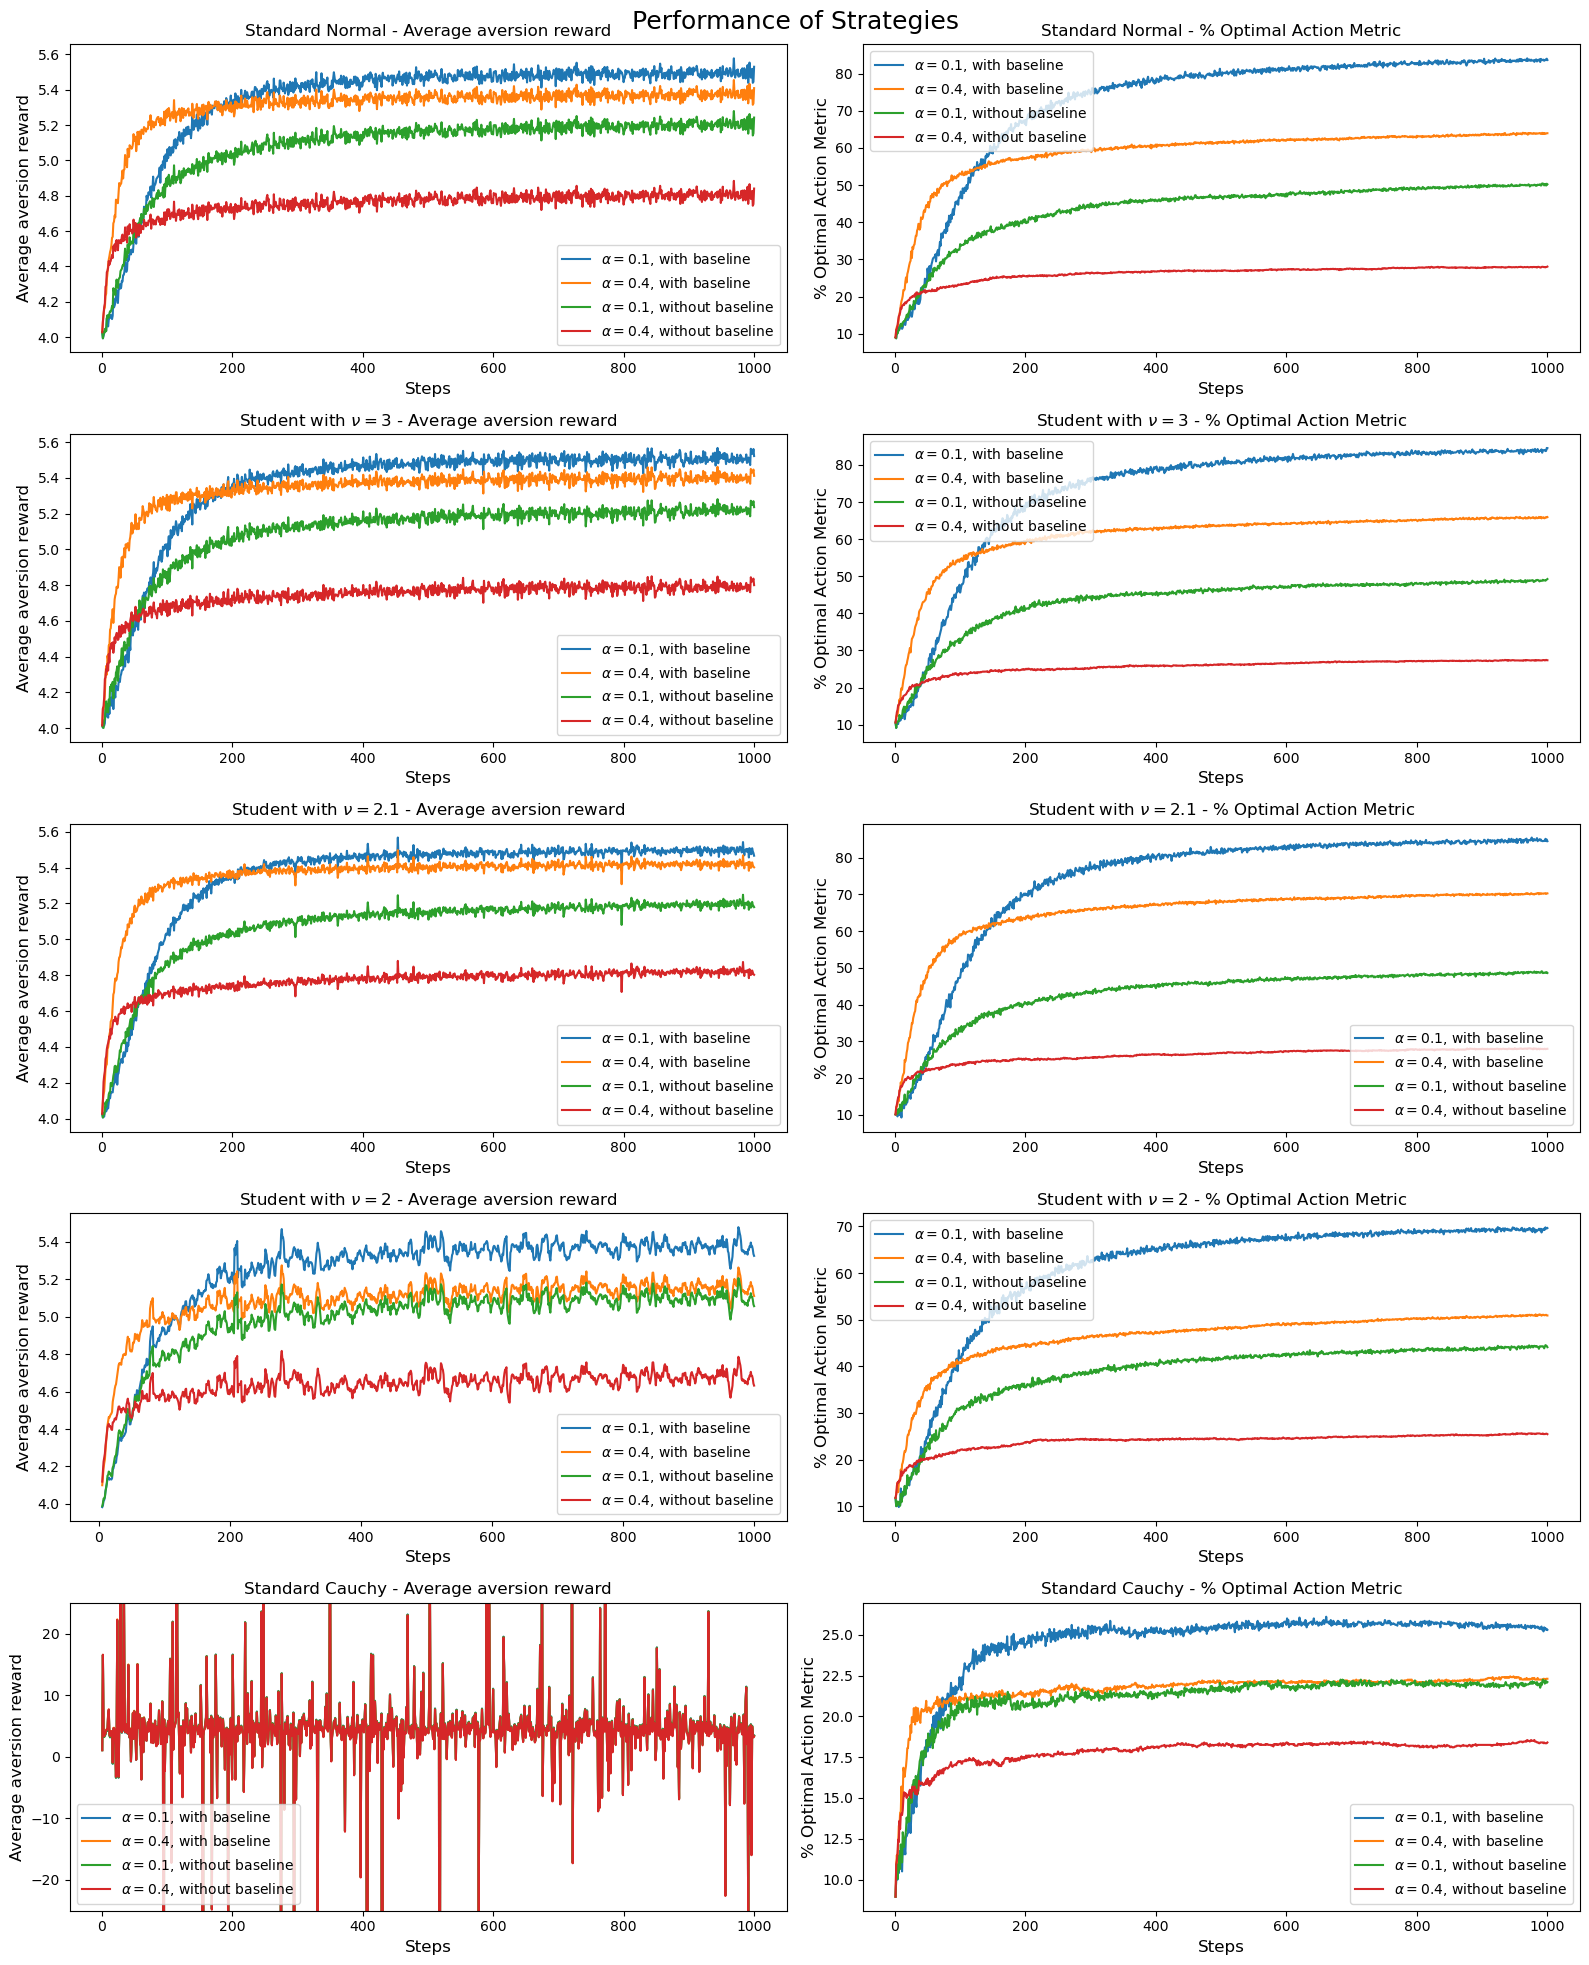
\includegraphics[width=1.1\linewidth]{Figures/experiments_classic/gradient_bandits/first.png}
    \caption{\label{fig:gradient_1}Значения средней награды и процента оптимального выбора для gradient bandits, сгруппировано по распределениям. Меньшее $\alpha$ и присутствие baseline приводят к лучшим результатам}
\end{figure}
\begin{figure}[ht!]
    \centering
    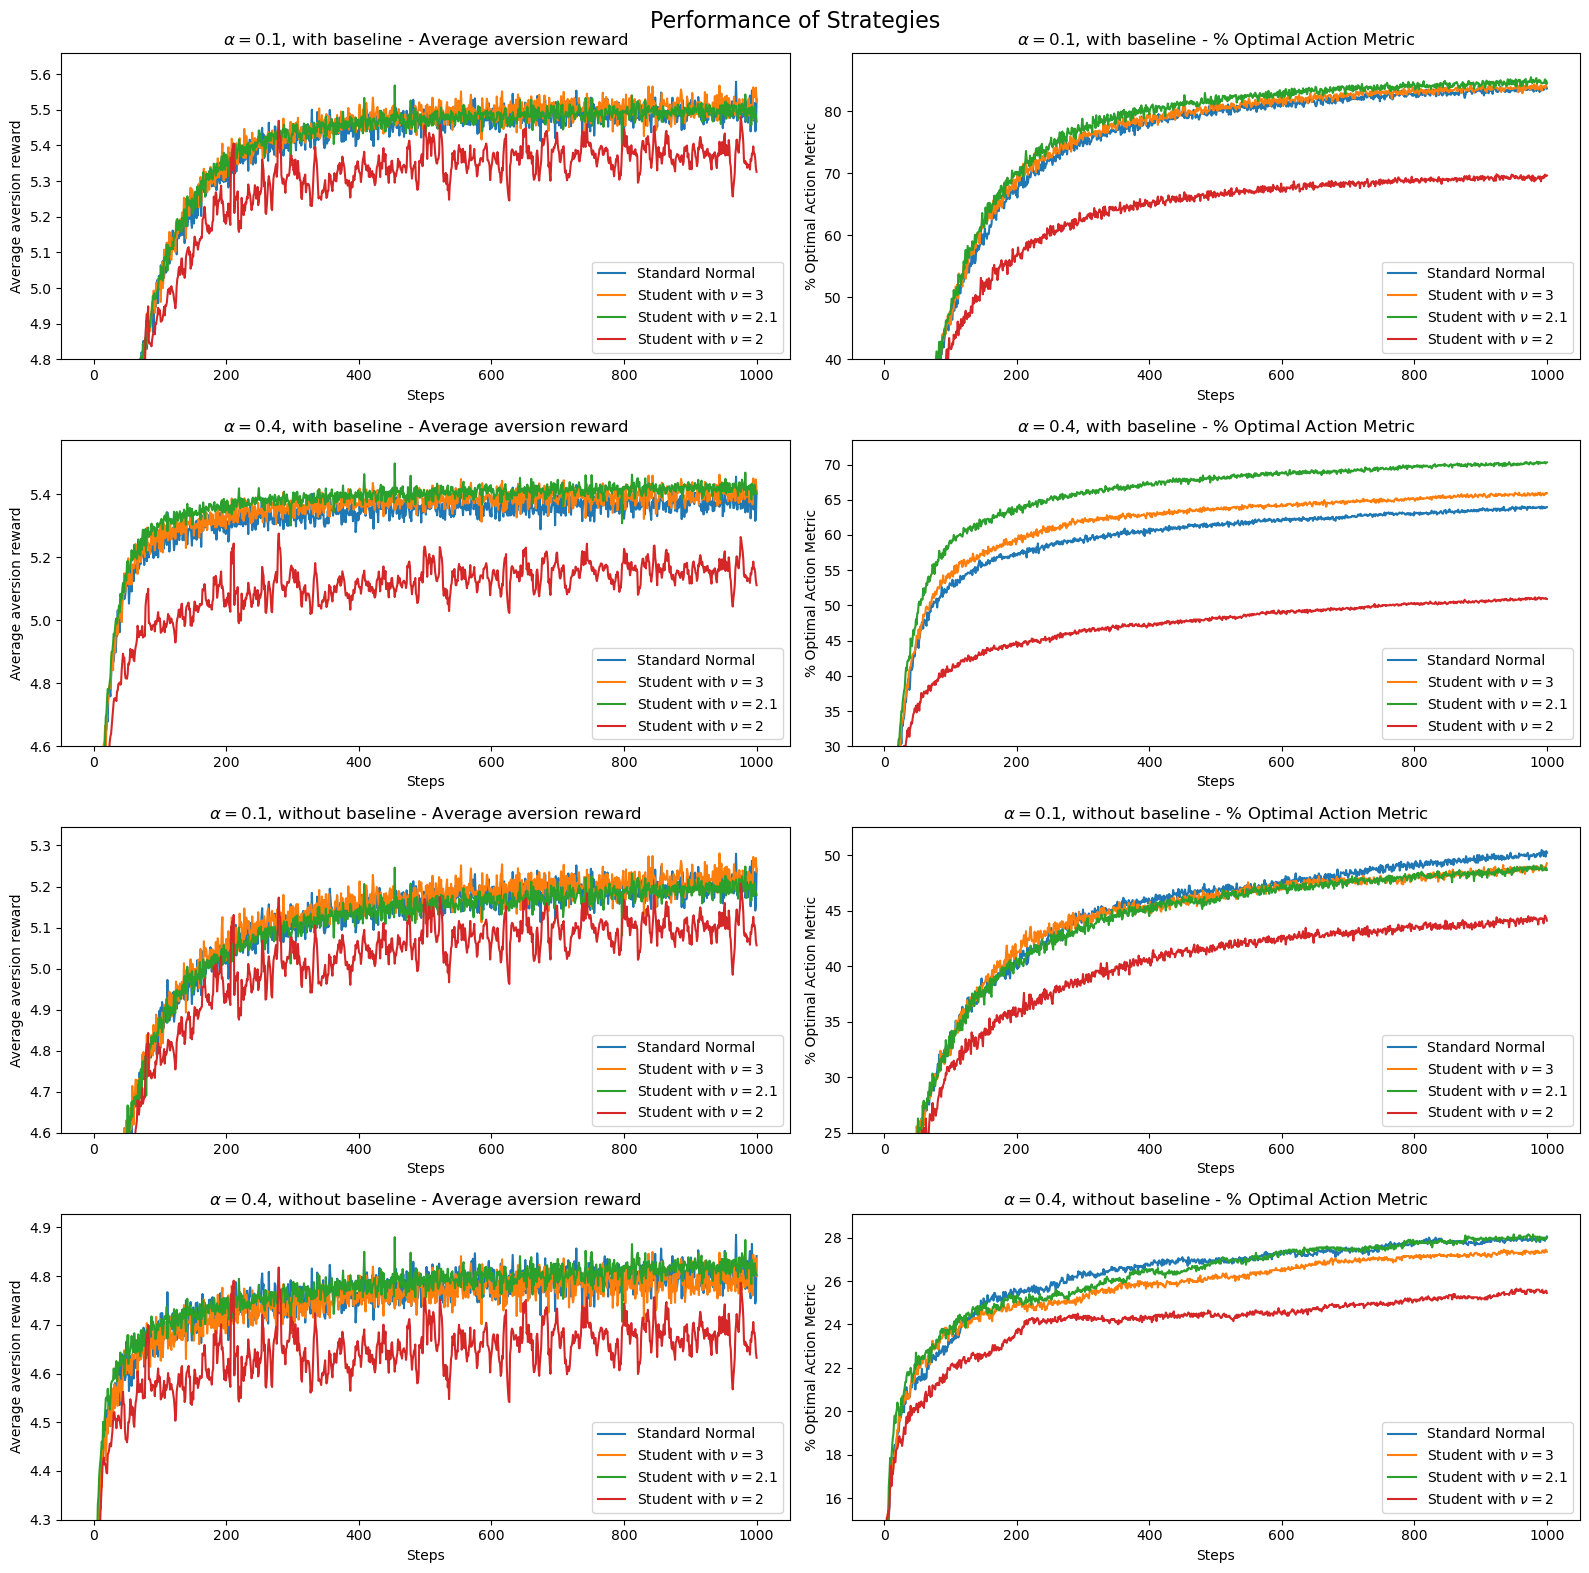
\includegraphics[width=1.1\linewidth]{Figures/experiments_classic/gradient_bandits/second.png}
    \caption{\label{fig:gradient_2}Значения средней награды и процента оптимального выбора для gradient bandits, сгруппировано по стратегиям. Заметно странное поведение метрик: когда есть baseline, значения для $t_{2.1}$ лучше, чем для $t_{3}$}.
\end{figure}

\section{Сравнение всех стратегий}

В целом, характерны следующие тенденции:
\begin{enumerate}
    \item У $t_2$ имеются резкие перепады в средней награде с сохранением тенденции к увеличению (или уменьшению для постоянного step-size). Это объясняется отсутсвием у $t_2$ дисперсии.
    \item Везде, кроме greedy стратегий и стратегий с постоянным step-size, занчения метрик для $t_{\infty}$ и $t_3$ почти совпадают, то есть стратегии одинаково применимы для этих двух распределений.
\end{enumerate}

Наконец, проанализируем графики со сравнениями всех стратегий. Для всех распределений лучшую среднюю награду и процент оптимальных действий выдает UCB. Хотя для $t_{\infty}$ жадная позитивная инициализация идет второй по итоговому значению и лишь немного уступает UCB, заметна тенденция падения относительно других стратегий максимального значения для жадной позитивной инициализации с постоянным step-size при уменьшающемся $\nu$. На всех графиках, кроме $t_1$, градиентные бандиты показывают себя немного лучше, чем $\epsilon$-greedy. Как уже было сказано, график средней награды для распределения Коши не имеет смысла, для процента оптимальных действий лучшие значения достигаются для $\epsilon$-greedy и UCB, при этом значения метрики для gradient bandits значительно падают относительно этих стратегий. Так происходит, поскольку baseline есть среднее по всем предыдущим шагам, что не сходится ни к какому значению при любом распределении выбора действий.

В целом UCB на всех распределениях показывает лучший или один из лучших результатов, что можно объяснить тем, что эта стратегия дает любому рычагу воможность быть выбранным, при этом эта вероятность быть выбранным уменьшается с увеличением числа шагов и при этом в меньшей степени привязана к матожиданию, как, например, gradient bandits. Так как так же дается ненулевая вероятность быть выбранным каждому рычагу, $\epsilon$-greedy и gradient bandits тоже дают хорошие результаты на $t_2, t_{2.1}, t_3, t_{\infty}$.

\begin{figure}[ht!]
    \centering
    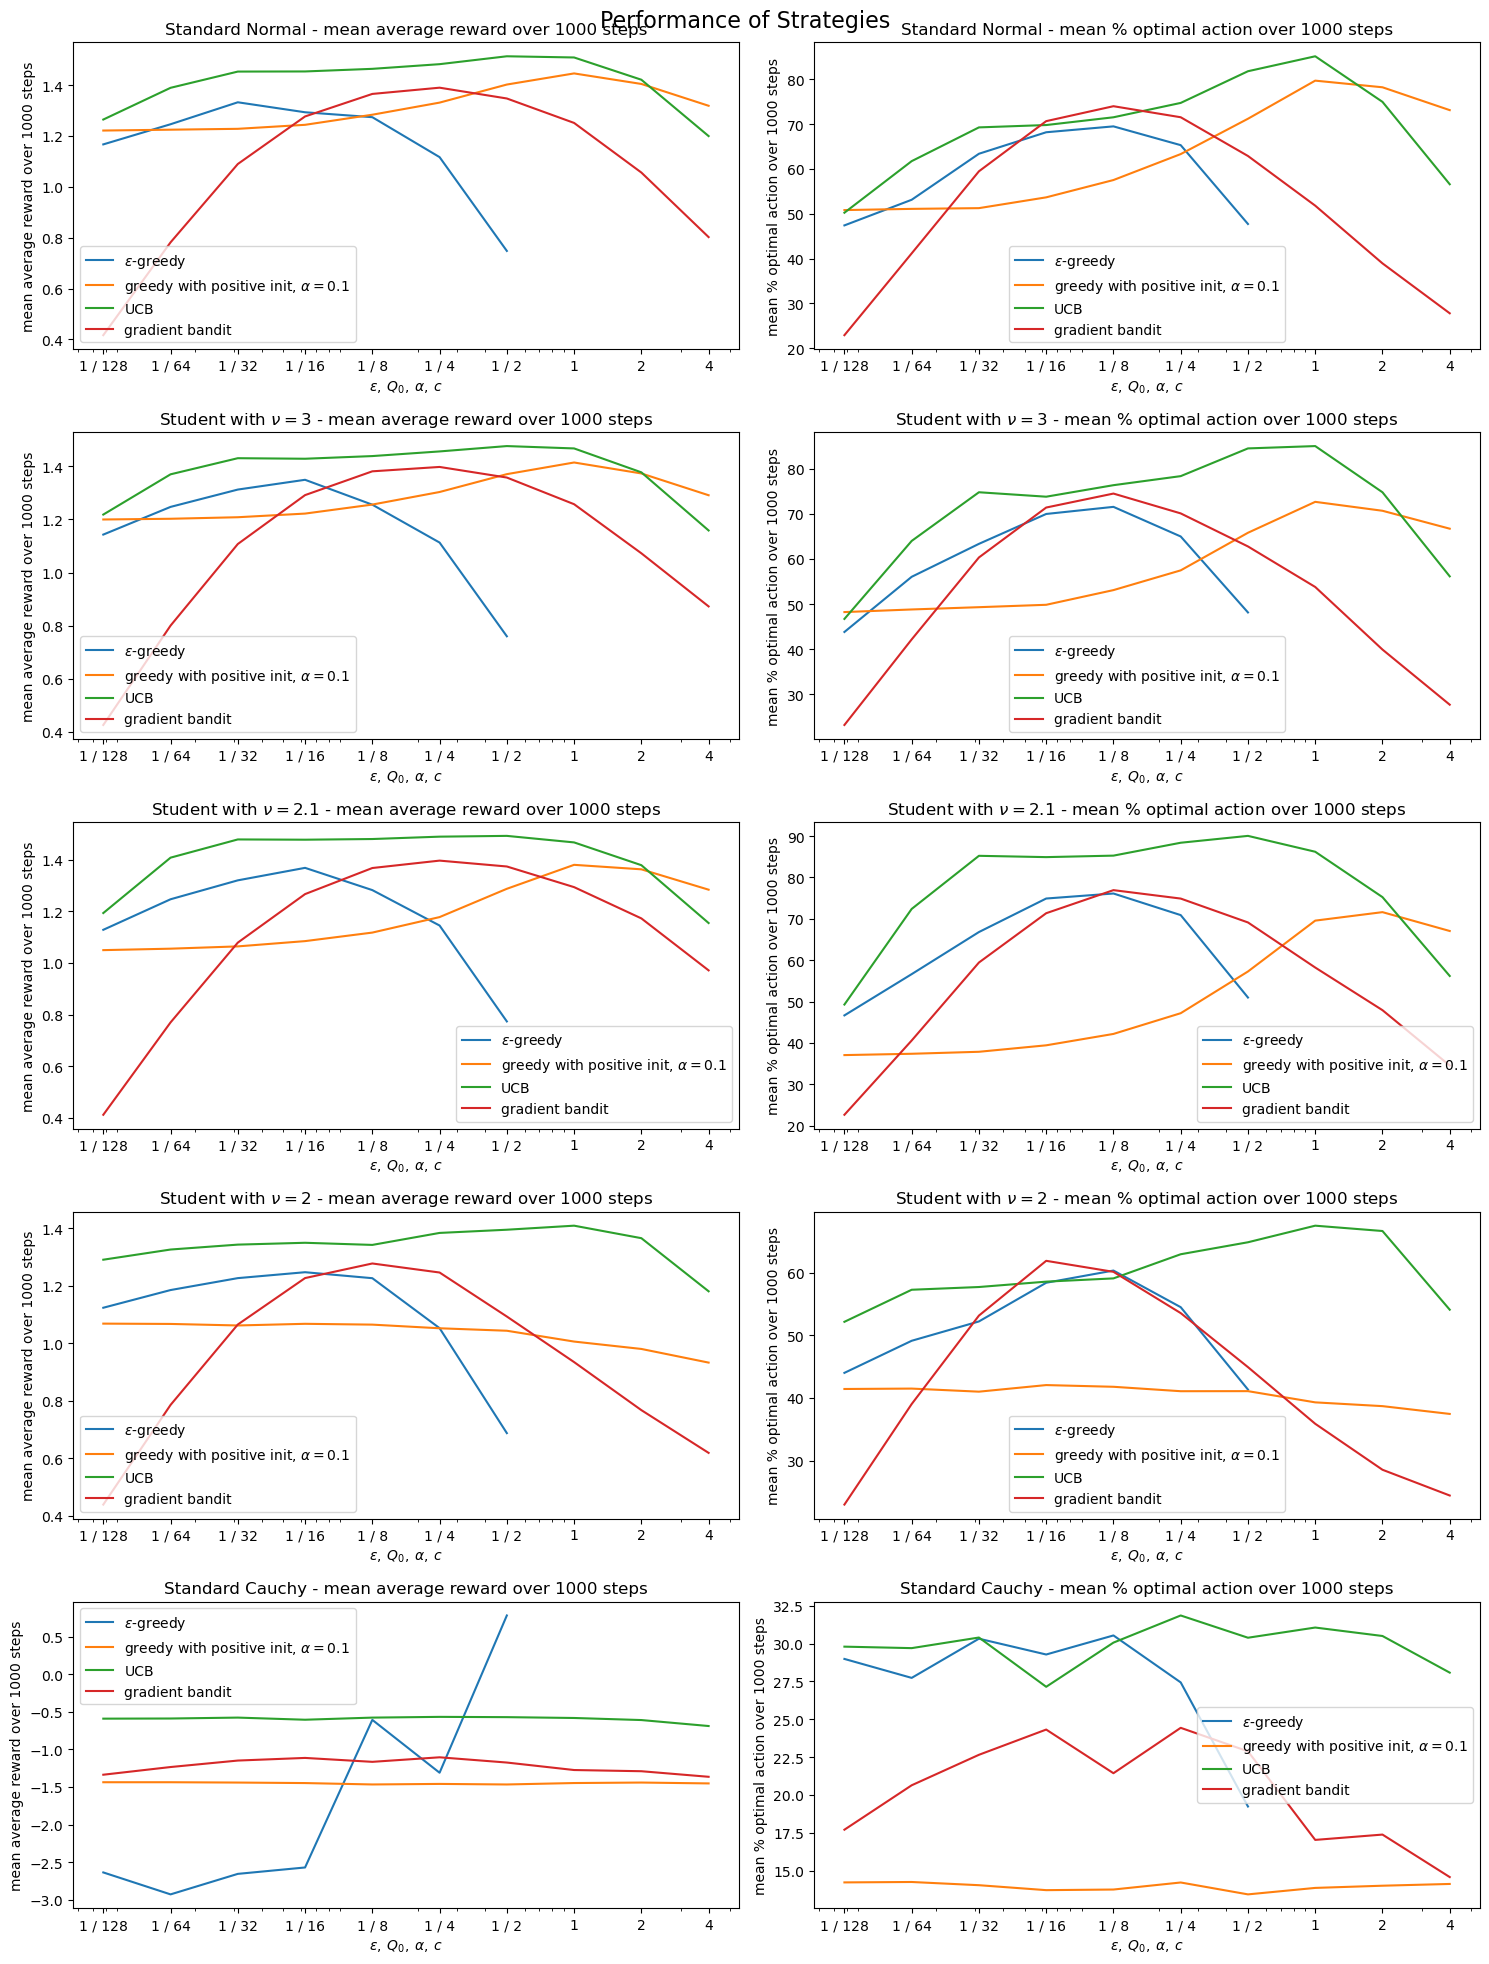
\includegraphics[width=1.1\linewidth]{experiments_classic/overall/overall.png}
    \caption{\label{fig:overall}Сравнение всех стратегий при варьировании гиперпараметров}
\end{figure}

\section{Выводы}

Проделанные эксперименты позволяют судить о том, что Gradient bandits, $\epsilon$-greedy и UCB -- стратегии показывают высокую эффективность на степенных распределениях. Так как UCB -- единственная из стратегий, показывающая высокую эффективность на всех метриках и всех распределениях, то эта стратегия, при условии, что существует способ адаптации доверительного интервала для дисперсии -- лучший кандидат на применение в задаче о многоруких бандитах с учетом отвращения к риску.
% Chapter Template

\chapter{Эксперименты для задачи с учетом неприятия к риску} % Main chapter title

\label{ExperimentsAversion} % Change X to a consecutive number; for referencing this chapter elsewhere, use \ref{ChapterX}

%----------------------------------------------------------------------------------------
%	SECTION 1
%----------------------------------------------------------------------------------------

\section{Проверка greedy-алгоритмов}

Для начала была проведена проверка 2 алгоритмов для нахождения решения задачи в случае, когда все матожидания и дисперсии известны. Первый алгоритм -- алгоритм StandardGreedy. Второй алгоритм -- алгоритм градиентного подъема CauchySimplex, представленный в \cite{cauchy_simplex}. Среди неградиентных методов был рассмотрен только метод StandardGreedy, поскольку он обладает самой меньшей алгоритмической сложностью шага $O(n \log n)$. В CauchySimplex выбраны такие гиперпараметры: $\epsilon = 10^{-3}$, $stop = 10^{-9}$ -- когда изменение $V = \sum_{i=1}^n p_i m_i - \lambda \sum_{i=1}^n p_i^2 \sigma_i^2$ за один шаг меньше, чем $stop$, то алгоритм останавливается (см. \ref{fig:cauchy_simplex}). \\

Далее происходит запуск 500 тестов, в каждом тесте было 10 распределений со средними, выбранными случайно из $\mathcal{N}(1,1)$, и дисперсиями $\sigma^2$, т.ч. $\sigma \sim Exp(2)$.  Чтобы включить среди рычагов ``безрисковые'' рычаги, каждая из дисперсий с вероятностью $\frac{1}{n}$ ($n=10$) домножалось на 0. Для каждого такого набора матожиданий и дисперсий запускались алгоритмы StandardGreedy и CauchySimplex, после чего полученные вероятности сравнивались. Если хотя бы 2 вероятности отличаются больше, чем на гиперпараметр error\_rate, тест считался проваленным. Алгоритм, сравнивающий подходы, был запущен 2 раза для error\_rate$=0.02$ и error\_rate$=0.05$. \\

В результате при error\_rate$=0.02$ количество проваленных тестов равнялось $2.8\%$, а при error\_rate$=0.05$ все тесты прошли успешно (см. \ref{fig:comparison_standard_greedy_cauchy_simplex}). При этом среднее выполнение CauchySimplex составляет от 90 до 160 миллисекунд, в то время как StandardGreedy -- меньше $0.1$ миллисекунды. Это позволяет сделать 3 вывода:
\begin{enumerate}
    \item Ввиду того, что CauchySimplex относится к градиентным методам и потому обладает некоторой погрешностью, и этот алгоритм выдает оптимальное решение, то и алгоритм StandardGreedy выдает оптимальное решение.
    \item Погрешность метода CauchySimplex иногда достаточно большая.
    \item Алгоритм StandardGreedy намного быстрее CauchySimplex.
\end{enumerate}
На основании этого можно сделать вывод, что StandardGreedy более применим для проведения экспериментов.

\begin{figure}[ht!] %!t
\centering
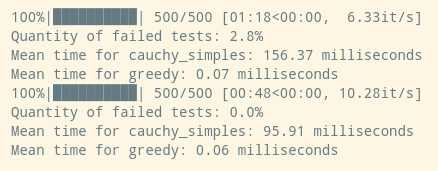
\includegraphics[width=4in]{theory_tester/theory_images/results_compare.png}
\caption{Результаты сравнения алгоритмов CauchySimplex и StandardGreedy}
\label{fig:comparison_standard_greedy_cauchy_simplex}
\end{figure}

\section{Параметры}

Набор используемых семейств распределений дан в таблице \ref{table:aversion_distribution_family}. Число $a$ для каждого рычага сэмплируется из $\mathcal{N}(1,1)$ (за исключением градиентных бандитов, чтобы продемонстрировать их невосприимичвость к изменению среднего). Параметр растяжения $\sigma$ для каждого рычага был взят из $\sigma \sim Exp(2)$. Таким образом, при $\nu > 2$ дисперсия каждого рычага равна $\sigma^2$. Чтобы включить среди рычагов ``безрисковые'' рычаги, после домножения на $\sigma$ каждое из распределений с вероятностью $\frac{1}{n}$ ($n=10$) домножалось на 0. Таким образом, с вероятностью примерно $1 - e^{-1} \approx 63\%$ среди рычагов есть хотя бы один с нулевой дисперсией. Хотя для $t_2$ цель максимизации $\sum_{i=1}^n p_i m_i - \lambda \sum_{i=1}^n p_i^2 \sigma_i^2$ некорректна, поскольку у $t_2$ нет дисперсии, можно вместо дисперсии $\sigma^2$ подставить параметр растяжения $\sigma_{\text{scale}}^2$, возведенный в квадрат, то есть пытаться найти $\sum_{i=1}^n p_i m_i - \lambda \sum_{i=1}^n p_i^2 \sigma_{i, \text{scale}}^2$. Естественно, вся разработанная до этого теория не работает для максимизации измененной величины.

Списки отдельных экспериментов с применяемыми в них стратегиями даны в таблицах \ref{table:aversion_greedy}, \ref{table:aversion_adaptive}, \ref{table:aversion_positive}, \ref{table:aversion_ucb}, \ref{table:aversion_gradient_bandits}. Кроме того, были протестированы $\epsilon$-greedy стратегии с $\epsilon=0.1$ и скорректированной дисперсией. Об этом подробнее в разделе~\ref{sec:correction_eps_greedy}. Список гиперпараметров дан в таблице \ref{table:classic_hyperparameters}.

В качестве метрик взяты:
\begin{enumerate}
    \item $\text{Regret} = \left( \sum_{i=1}^n p_i^* m_i - \lambda \sum_{i=1}^n (p_i^*)^2 \sigma_i^2 \right) - \left( \sum_{i=1}^n p_i Q_t(i) - \lambda \sum_{i=1}^n (p_i)^2 S_t^2(i) \right)$ -- среднее сожаление, где $\textbf{p}^*$ -- решение исходной задачи
    \item $\text{Regret}_{{\text{real}}} = \left( \sum_{i=1}^n p_i^* m_i - \lambda \sum_{i=1}^n (p_i^*)^2 \sigma_i^2 \right) - \left( \sum_{i=1}^n p_i m_i - \lambda \sum_{i=1}^n (p_i)^2 \sigma_i^2 \right)$ -- среднее реальное сожаление.
    \item Процент выбранных оптимальных действий на каждом шаге $Opt = 1 - 2 \sum_{i=1}^n |p_i - p_i^*|$. Заметим, что в обычной задаче о многоруких бандитах $P = (0, ..., 1, 0, ..., 0)$, и новая метрика равна 
    \[
    1 - \frac{1}{2}\left( (1 - b_k) + \sum_{i = 1, i \neq k}^n b_i \right) = 1 - (1 - b_k) = b_k
    \]
    то есть совпадает с процентом оптимальных действий, а это есть вторая метрика в обычной задаче о многоруких бандитах.
\end{enumerate}
В качестве вероятности $p$ в метрики будем подставлять ту вероятность, из которой в данный шаг происходит выбор рычага (то есть, например, для $\epsilon$-greedy, если выбор происходил случайно, то в метрику подставлялся вектор $\left( \frac{1}{n}, ..., \frac{1}{n} \right)$, хотя внутри себя стратегия хранит другое значение вероятностей). Выбор в пользу такого варианта был сделан, поскольку нам важно, на какие рычаги в реальности происходят нажатия, а не то, какая стратегия когда-то будет использоваться, то есть важна ``стоимость'' обучения. Для каждого распределения и каждой метрики результаты для одной группы стратегий визуализированы на графике. Кроме того, для каждой стратегии и для каждой метрики на одном графике были изображены результаты по всем распределениям.
 
Так как коэффициент отвращения к риску $\lambda$ также может влиять на эффективность алгоритмов, то будем дополнительно строить графики зависимости метрик от числа шагов для разных распределений и для одной фиксированной стратегии. Дополнительно построим график средних значений метрик на последних 5 шагах от $\lambda$ в зависимости от распределения, чтобы понять изменение конечного результата работы алгоритмов в зависимости от важности риска. Для оценки были взяты $\lambda \in [0.01, 0.05, 0.12, 0.3, 0.6, 1, 2, 4, 10]$.

\begin{table}
\centering
\renewcommand{\arraystretch}{1.5}
\begin{tabular}{ |m{4cm}||m{2.1cm}|m{6cm}|  }
 \hline
 \multicolumn{3}{|c|}{Список используемых распределений} \\
 \hline
 Распределение & Обозначение & Плотность $p(x)$ \\
 \hline
  Нормальное   &  $t_{\infty} $&  $\frac{1}{\sqrt{2\pi \sigma^2}}e^{\frac{(x-a)^2}{2\sigma^2}}$ \\
 \hline
 Стьюдента с $\nu=3$ нормированное & $t_{3}$ & $\frac{1}{\sqrt{3}} \cdot \frac{2}{\pi \sqrt{3\sigma^2} \left( 1 + \frac{(x-a)^2}{3\sigma^2} \right)^2}$ \\
 \hline
 Стьюдента с $\nu=2.1$ нормированное & $t_{2.1}$ & $\frac{1}{\sqrt{21}} \cdot \frac{\Gamma(1.55)}{\sqrt{2.1 \pi \sigma^2} \Gamma(1.05)} \left( 1 + \frac{(x-a)^2}{2.1 \sigma^2} \right)^{-1.55}$ \\
 \hline
 Стьюдента с $\nu=2$ & $t_2$ & $\frac{1}{2\sqrt{2\sigma^2} \left( 1 + \frac{(x-a)^2}{2\sigma^2} \right)^{3/2}}$ \\
 \hline
\end{tabular}
\caption{Список семейств распределений для проверки стратегий в измененной задаче о многоруких бандитах. Рычаги каждый раз берутся из одного семейства.}
\label{table:aversion_distribution_family}
\end{table}


\begin{table}
\centering
\renewcommand{\arraystretch}{1.3}
\begin{tabular}{ |m{3cm}|m{5cm}|  }
 \hline
 \multicolumn{2}{|c|}{Тест $\epsilon$-greedy ($\forall a \hook Q_1(a) = \overline{R_1^2(a)} = 0$)} \\
 \hline
 Стратегия & Параметры \\
 \hline
  Жадная   &  $\epsilon = 0$ \\
 \hline
 $\epsilon$-жадная & $\epsilon = 0.01$ \\
 \hline
 $\epsilon$-жадная & $\epsilon = 0.1$ \\
 \hline
\end{tabular}
\caption{Параметры для теста жадной и $\epsilon$-жадной стратегий в измененной задаче}
\label{table:aversion_greedy}
\end{table}

\begin{table}
\centering
\renewcommand{\arraystretch}{1.3}
\begin{tabular}{ |m{3cm}|m{5cm}|  }
 \hline
 \multicolumn{2}{|c|}{Тест стратегий с адаптивным $\epsilon$ ($\forall a \hook Q_1(a) = \overline{R_1^2(a)} = 0$)} \\
 \hline
 Стратегия & Параметры \\
 \hline
 $\epsilon$-жадная & $\epsilon = 0.1$ \\
 \hline
 Adaptive-$\epsilon$   &  $\epsilon_0 = 1$ \\
 \hline
 Adaptive-$\epsilon$ & $\epsilon_0 = 10$ \\
 \hline
 VDBE & $\epsilon_0 = 1, \, \delta = 0.1, \, \tau = 1$ \\
 \hline
 VDBE & $\epsilon_0 = 10, \, \delta = 0.1, \, \tau = 1$ \\
 \hline
\end{tabular}
\caption{Параметры для теста стратегий с адаптивным $\epsilon$ в измененной задаче}
\label{table:aversion_adaptive}
\end{table}

\begin{table}
\centering
\renewcommand{\arraystretch}{1.3}
\begin{tabular}{ |m{4cm}|m{5cm}|  }
 \hline
 \multicolumn{2}{|c|}{Тест позитивной инициализации} \\
 \hline
 Стратегия & Параметры \\
 \hline
 $\epsilon$-жадная & $\epsilon = 0.1, \: \forall a \hook Q_1(a) = \overline{R_1^2(a)} = 0$ \\
 \hline
 Жадная оптимистичная & $\epsilon = 0, \: \forall a \hook x_0(a) = 6$ \\
 \hline
 $\epsilon$-жадная оптимистичная & $\epsilon = 0.1, \: \forall a \hook x_o(a) = 6$ \\
 \hline
\end{tabular}
\caption{Параметры для теста стратегий с позитивной инициализацией в измененной задаче}
\label{table:aversion_positive}
\end{table}

\begin{table}
\centering
\renewcommand{\arraystretch}{1.3}
\begin{tabular}{ |m{3cm}|m{4cm}|  }
 \hline
 \multicolumn{2}{|c|}{Тест UCB ($\forall a \hook Q_1(a) = \overline{R_1^2(a)} = 0$)} \\
 \hline
 Стратегия & Параметры \\
 \hline
 $\epsilon$-жадная & $\epsilon = 0.1$ \\
 \hline
 UCB & $c=2, \, \epsilon=0.001$ \\
 \hline
\end{tabular}
\caption{Параметры для теста UCB в измененной задаче}
\label{table:aversion_ucb}
\end{table}


\begin{table}
\centering
\renewcommand{\arraystretch}{1.3}
\begin{tabular}{ |m{4cm}|m{6cm}|  }
 \hline
 \multicolumn{2}{|c|}{Тест градиентных бандитов ($\forall a \hook Q_1(a) = \overline{R_1^2(a)} = 0, \, H_1(a) = 0, \, m_a \sim \mathcal{N}(5,1)$)} \\
 \hline
 Стратегия & Параметры \\
 \hline
 Градиентные бандиты & $\alpha=0.1, \text{baseline} = \bar{w_t}$ \\
 \hline
 Градиентные бандиты & $\alpha=0.1, \text{baseline} = 0$ \\
 \hline
 Градиентные бандиты & $\alpha=0.4, \text{baseline} = \bar{w_t}$ \\
 \hline
 Градиентные бандиты & $\alpha=0.4, \text{baseline} = 0$ \\
 \hline
\end{tabular}
\caption{Параметры для теста градиентных бандитов в измененной задаче}
\label{table:aversion_gradient_bandits}
\end{table}

\section{Результаты}

На всех результатах графики реального сожаления и процента оптимальных действий для распределения $t_2$ не имеет смысла ввиду отсутствия у распределения дисперсии.

\subsection{$\epsilon$-greedy}

В этом подходе получились следующие графики:

\begin{figure}[ht!] %!t
\centering
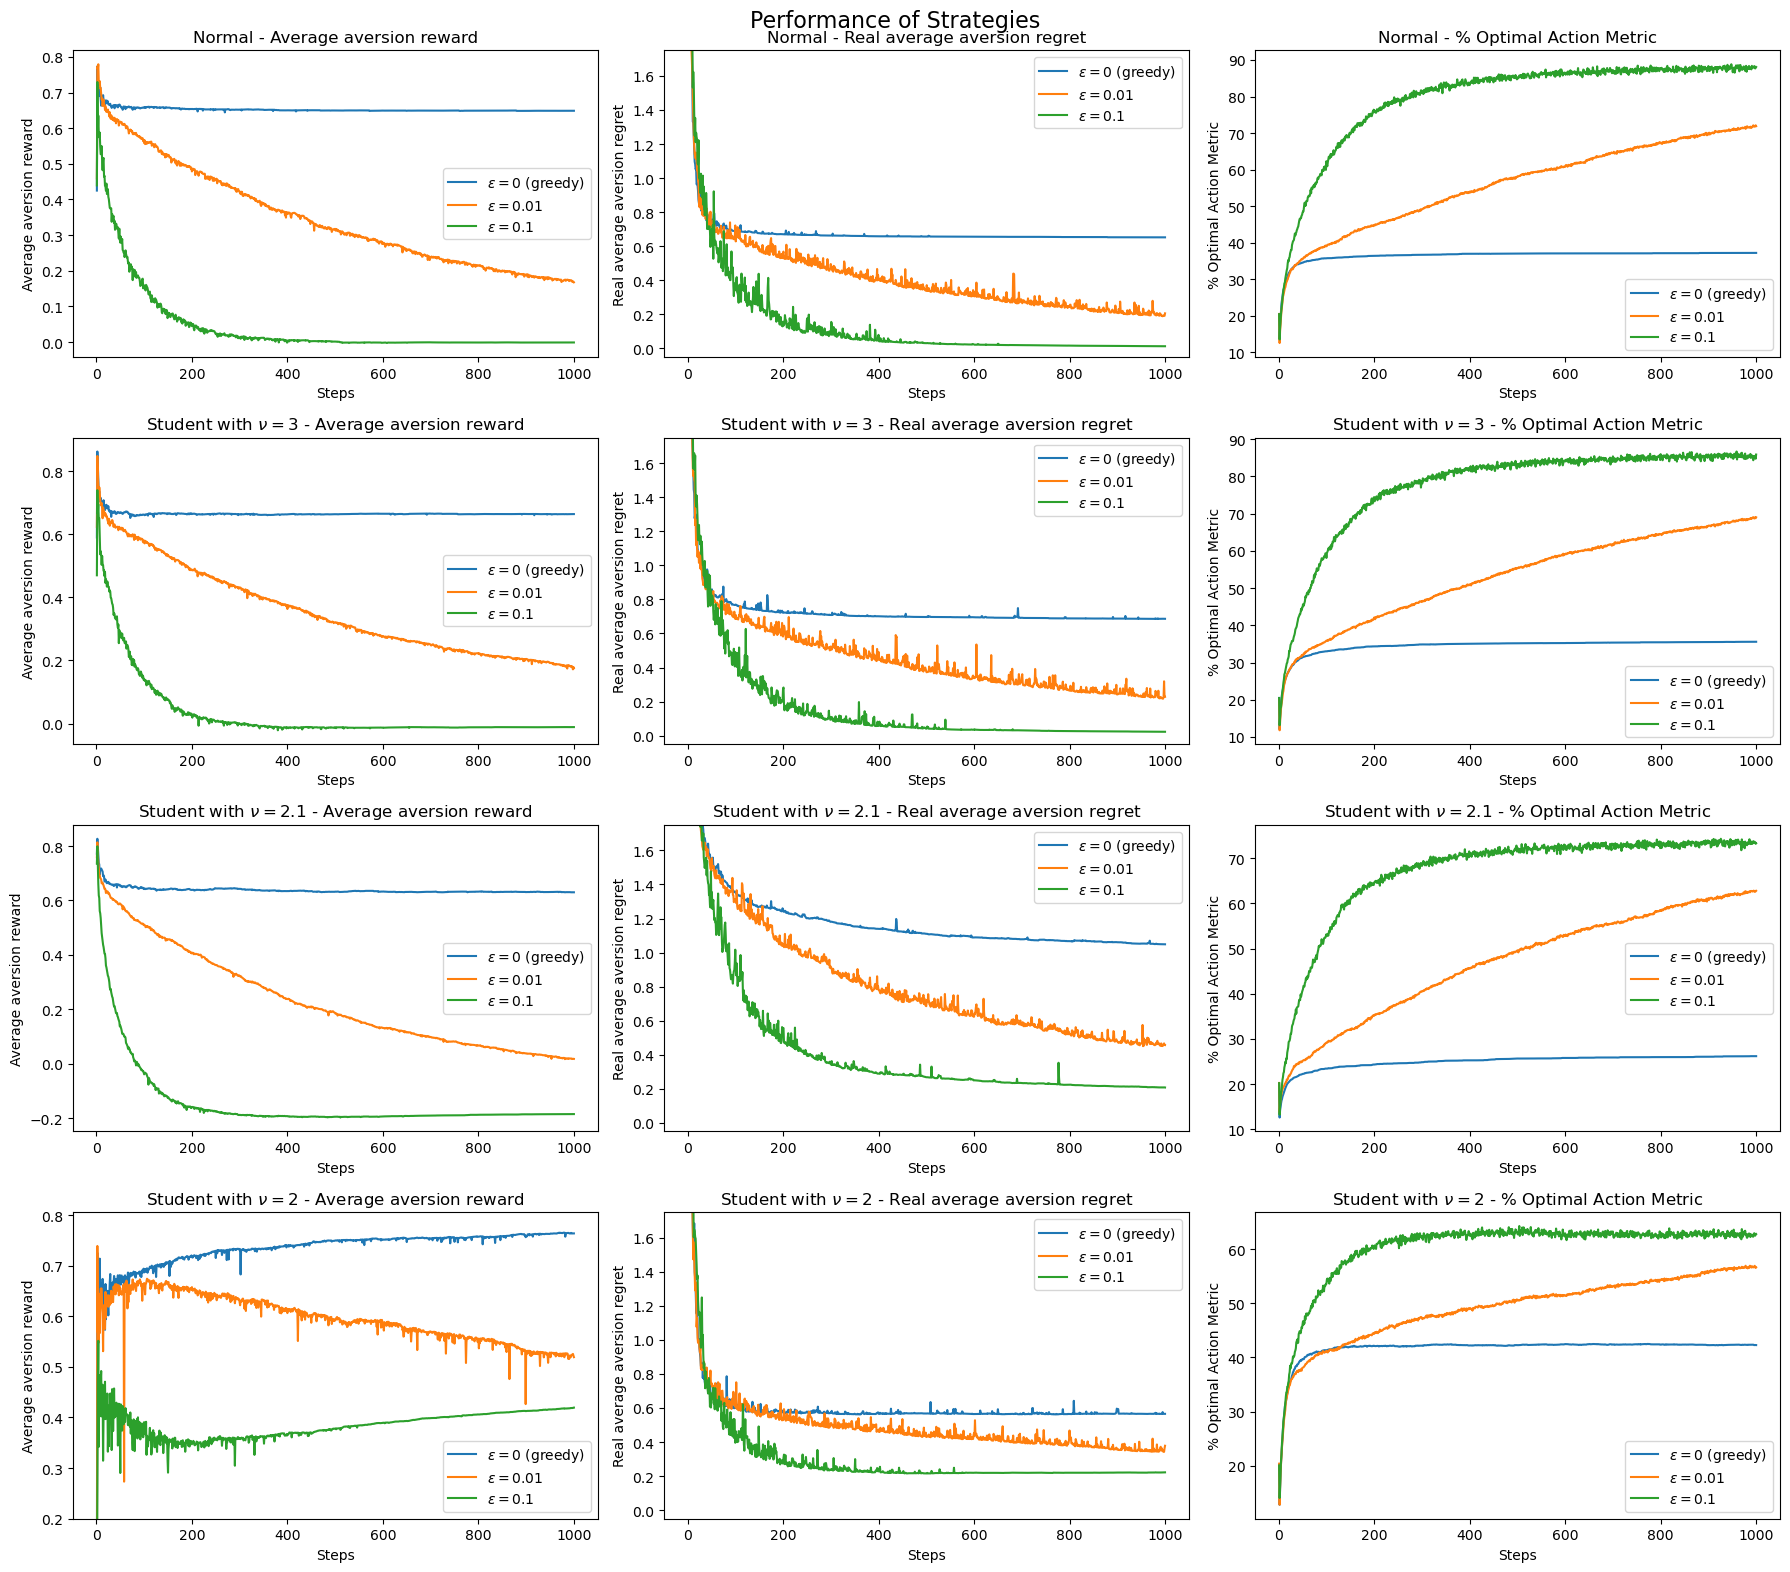
\includegraphics[width=6in]{theory_tester/theory_images/epsilon_greedy/strat_distr.png}
\caption{Зависимость метрик от количества шагов при greedy и $\epsilon$-greedy стратегиях для различных распределений}
\label{fig:epsilon_greedy_strat_distr}
\end{figure}

Хотя реальное сожаление не опускается ниже примерно $0.2$, алгоритм $\epsilon$-greedy выучивает с высокой точностью оптимальную стратегию, что можно видеть по следующему графику: 

Как можно видеть из \ref{fig:epsilon_greedy_strat_distr}, для любого распределения добавление случайного выбора улучшает exploration алгоритма, поэтому средние и дисперсии лучше приближаются, и ответ получается более близким к оптимальному. Например, для $t_{\infty}$ и $t_3$ и для $0.1$-greedy алгоритма процент оптимальных действий близок к $90\%$, почти достигая максимально возможного срднего значения в $91\%$. Также заметим, что для $t_{2.1}$ среднее значение сожаления Regret становится отрицательным, в то время как среднее реальное сожаление Regret$_{{\text{real}}}$ увеличилось на последних шагах до $0.4$ в отличие от $\approx 0.2$ для $t_3$. Это говорит о том, что алгоритм ``переоценивает'' себя, давая ``якобы'' лучше прибыль, чем оптимальное значения вероятности, из-за чего в реальности прибыль значительно ниже, чем для оптимальной вероятности.

Из-за чего это может происходить? Из-за недооценки значения дисперсии. Давайте смоделируем 10000 тестов, в каждом из них возьмем 1000 сэмплов из распределения Стьюдента с $t_{\nu}$ с дипсерсией 1, посчитаем выборочную дисперсию, а затем среди полученных 10000 выборочных дисперсий возьмем медиану. Эта медиана будет приближением медианы распределения выборочной дисперсии $s_{1000}^2$. Построим график зависимости этой медианы от числа степеней свободы при $\nu > 2$. Если бы мы считали выборочное матожидание вместо дисперсии, то ее медиана была бы постоянной и равнялась бы матожиданию $t_{\nu}$. В случае дисперсии все по-другому (см. \ref{fig:median_depend_on_df}):

\begin{figure}[ht!] %!t
\centering
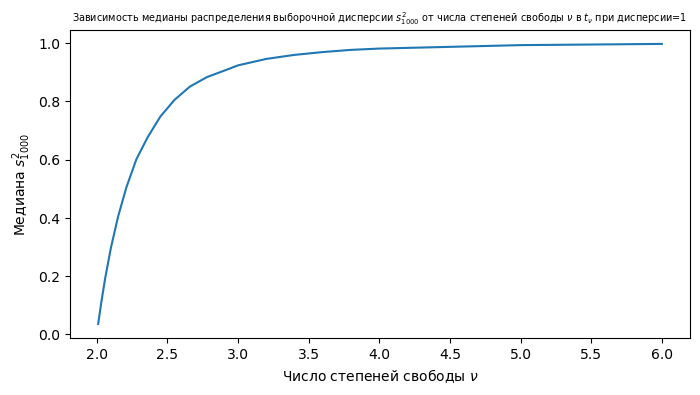
\includegraphics[width=5in]{theory_tester/theory_images/median_depend_on_df.png}
\caption{Зависимость медианы распределения выборочной дисперсии распределения Стьюдента $t_{\nu}$ относительно $\nu$}
\label{fig:median_depend_on_df}
\end{figure}

\begin{figure}[ht!] %!t
\centering
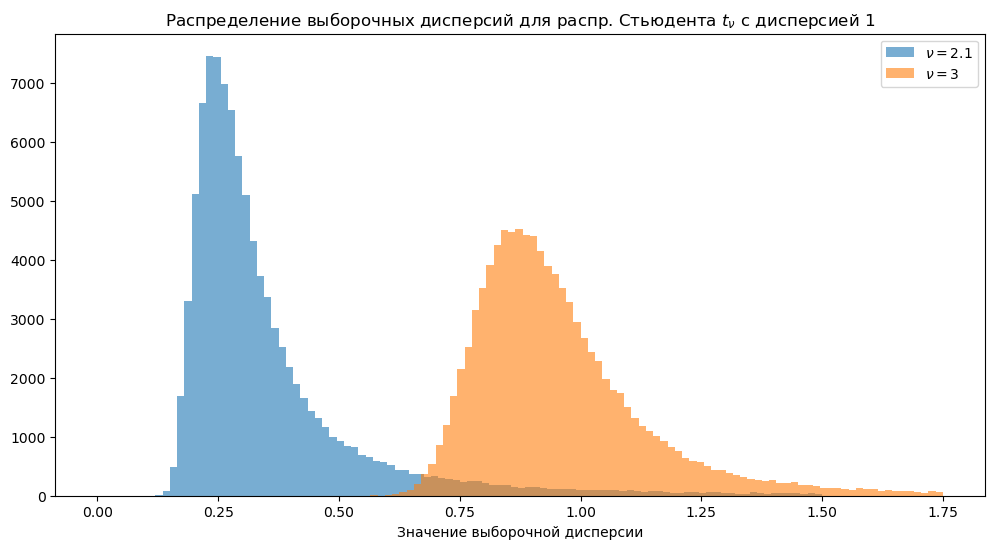
\includegraphics[width=5in]{theory_tester/theory_images/distributions_of_sample_variances.png}
\caption{Распределения выборочных дисперсий для распределений Стьюдента $\nu=2.1$ и $\nu=3$ с дисперсиями 1. Построено на 100000 значениях выборочной дисперсии $s_{1000}^2$}
\label{fig:distributions_of_sample_variances}
\end{figure}

Как можно видеть, медиана стремится к 0 при $\nu \to 2+$. При этом для любого $\nu$ медиана меньше среднего и медиана стремится к 1 при $\nu \to \infty$. В частности, при $\nu=2.1$ медиана примерно равна $0.3$, а при $\nu=3$ -- примерно равна $0.92$ (см. \ref{fig:distributions_of_sample_variances})

Это значит, что в большинстве случаев алгоритм недооценивает реальное значение дисперсии, из-за чего алгоритм склонен недооценивать риски и сосредотачивать деньги в активе с самой большой прибыльностью. А это, в свою очередь, снижает эффективность алгоритма. \label{negative_regret} Кроме того, поскольку дисперсии недооцениваются, то из прибыли вычитается меньшее значение, и потому алгоритм выдает большее значение прибыли, чем для оптимальной вероятности, что дает отрицательное среднее сожаление.

Что касается распределения Стьюдента $t_3$, то для него медианное значение дисперсии близко к реальному, поэтому эффект ``переоценки'' практически не проявляется.

Как мы выяснили, среди нарисованных на графике стратегий лучше всех работает $0.1$-greedy. Построим для нее график зависимости метрик от коэффциента отвращения для каждого распределения (\ref{fig:aversion_last_5_steps}):

\begin{figure}[ht!] %!t
\centering
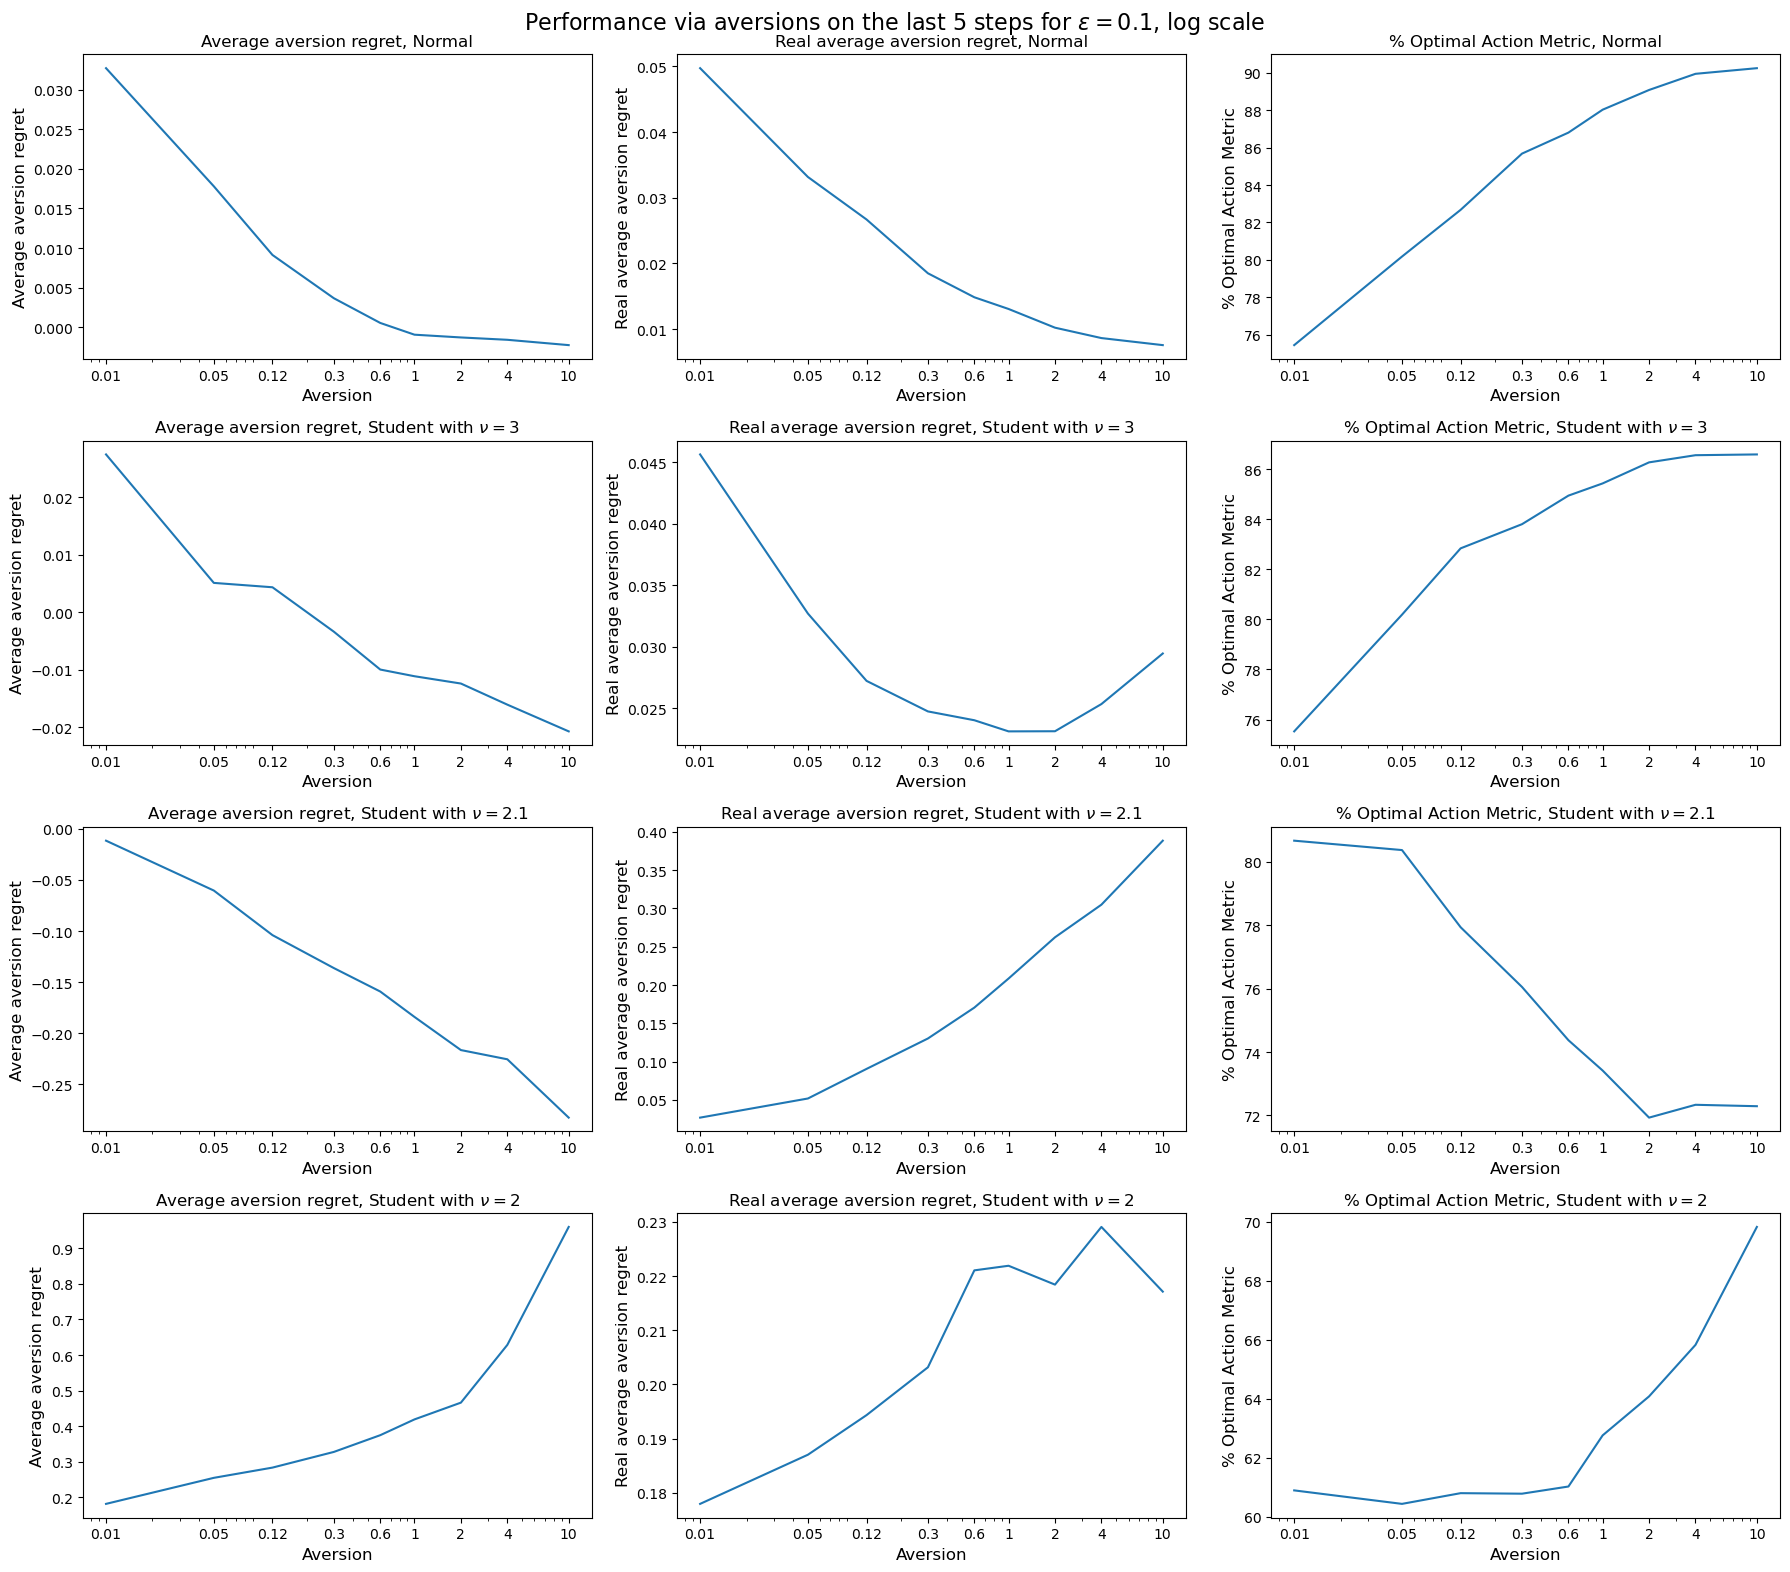
\includegraphics[width=6in]{theory_tester/theory_images/epsilon_greedy/aversion_last_5_steps.png}
\caption{График зависимости метрик от коэффциента отвращения для каждого распределения, усредненное по последним 5 шагам.}
\label{fig:aversion_last_5_steps}
\end{figure}

Как видно из графиков, для любого распределения с $\nu > 2$ при увеличении коэффициента отвращения к риску $\lambda$ метрика Regret уменьшается, и алгоритм переходит от своей недооценки к переоценке. Для $t_3$ и $t_{\infty}$ при увеличении $\lambda$ процент оптимальных действий увеличивается (хотя при $\nu = 3$ Regret$_{{\text{real}}}$ имеет минимум). В какой-то момент происходит переход, и для $t_{2.1}$ при уменьшении $\lambda$ точность увеличивается. Для $t_2$ при уменьшении $\lambda$ тоже наблюдается уменьшение Regret$_{{\text{real}}}$.

Почему при $\lambda \to 0+$ для больших степеней свободы эффективность алгоритма падает? При маленьких $\lambda$ дисперсия почти не учитывается при подсчете формулы, поэтому в оптимальном векторе вероятностей вся вероятность находится в рычаге с наибольшим матожиданием. Возьмем 2 рычага с наибольшим матожиданием $L_1$ и $L_2$ (у $L_1$ матожидание больше). Предположим, что у $L_1$ больше дисперсия, чем у $L_2$ (вероятность этого $\approx 0.5$). Тогда флуктуация получаемых наград у $L_2$ будет больше, чем у $L_1$, а это приводит к тому, что часто случается ситуация, при которой $Q_t(L_1) < Q_t(L_2)$. В таком случае в $91\%$ случаев $0.1$-greedy алгоритм будет выбирать $L_2$, что далеко от оптимального действия нажимать на рычаг $L_1$. При увеличении $\lambda$ этот недостаток нивелируется более равномерным распределением вероятностей по рычагам и потому более частым выбором $L_1$.

При $\nu$, близких к 2, описанный выше эффект начинает нивелировать эффект недооценки (преуменьшения) дисперсии: при больших $\lambda$ вероятности более равномерно распределяются по рычагам. Но алгоритм оценивает дисперсию каждого рычага значительно меньше, чем есть на самом деле, поэтому алгоритм старается сильнее концентрировать вероятности в одном рычаге, что дает отличие в векторах вероятностей и итоговое уменьшение эффективности. Далее мы на других графиках увидим, что такое поведение связано именно с преуменьшением дисперсии.

Уменьшение метрики Regret на графике для $t_{\infty}$ связано с уменьшением точности алгоритма при уменьшении $\lambda$, а для $t_{3}$ и $t_{2.1}$ это, опять-таки, происходит из-за преуменьшения дисперсии, как было уже сказано ранее \ref{negative_regret}.

\begin{figure}[ht!] %!t
\centering
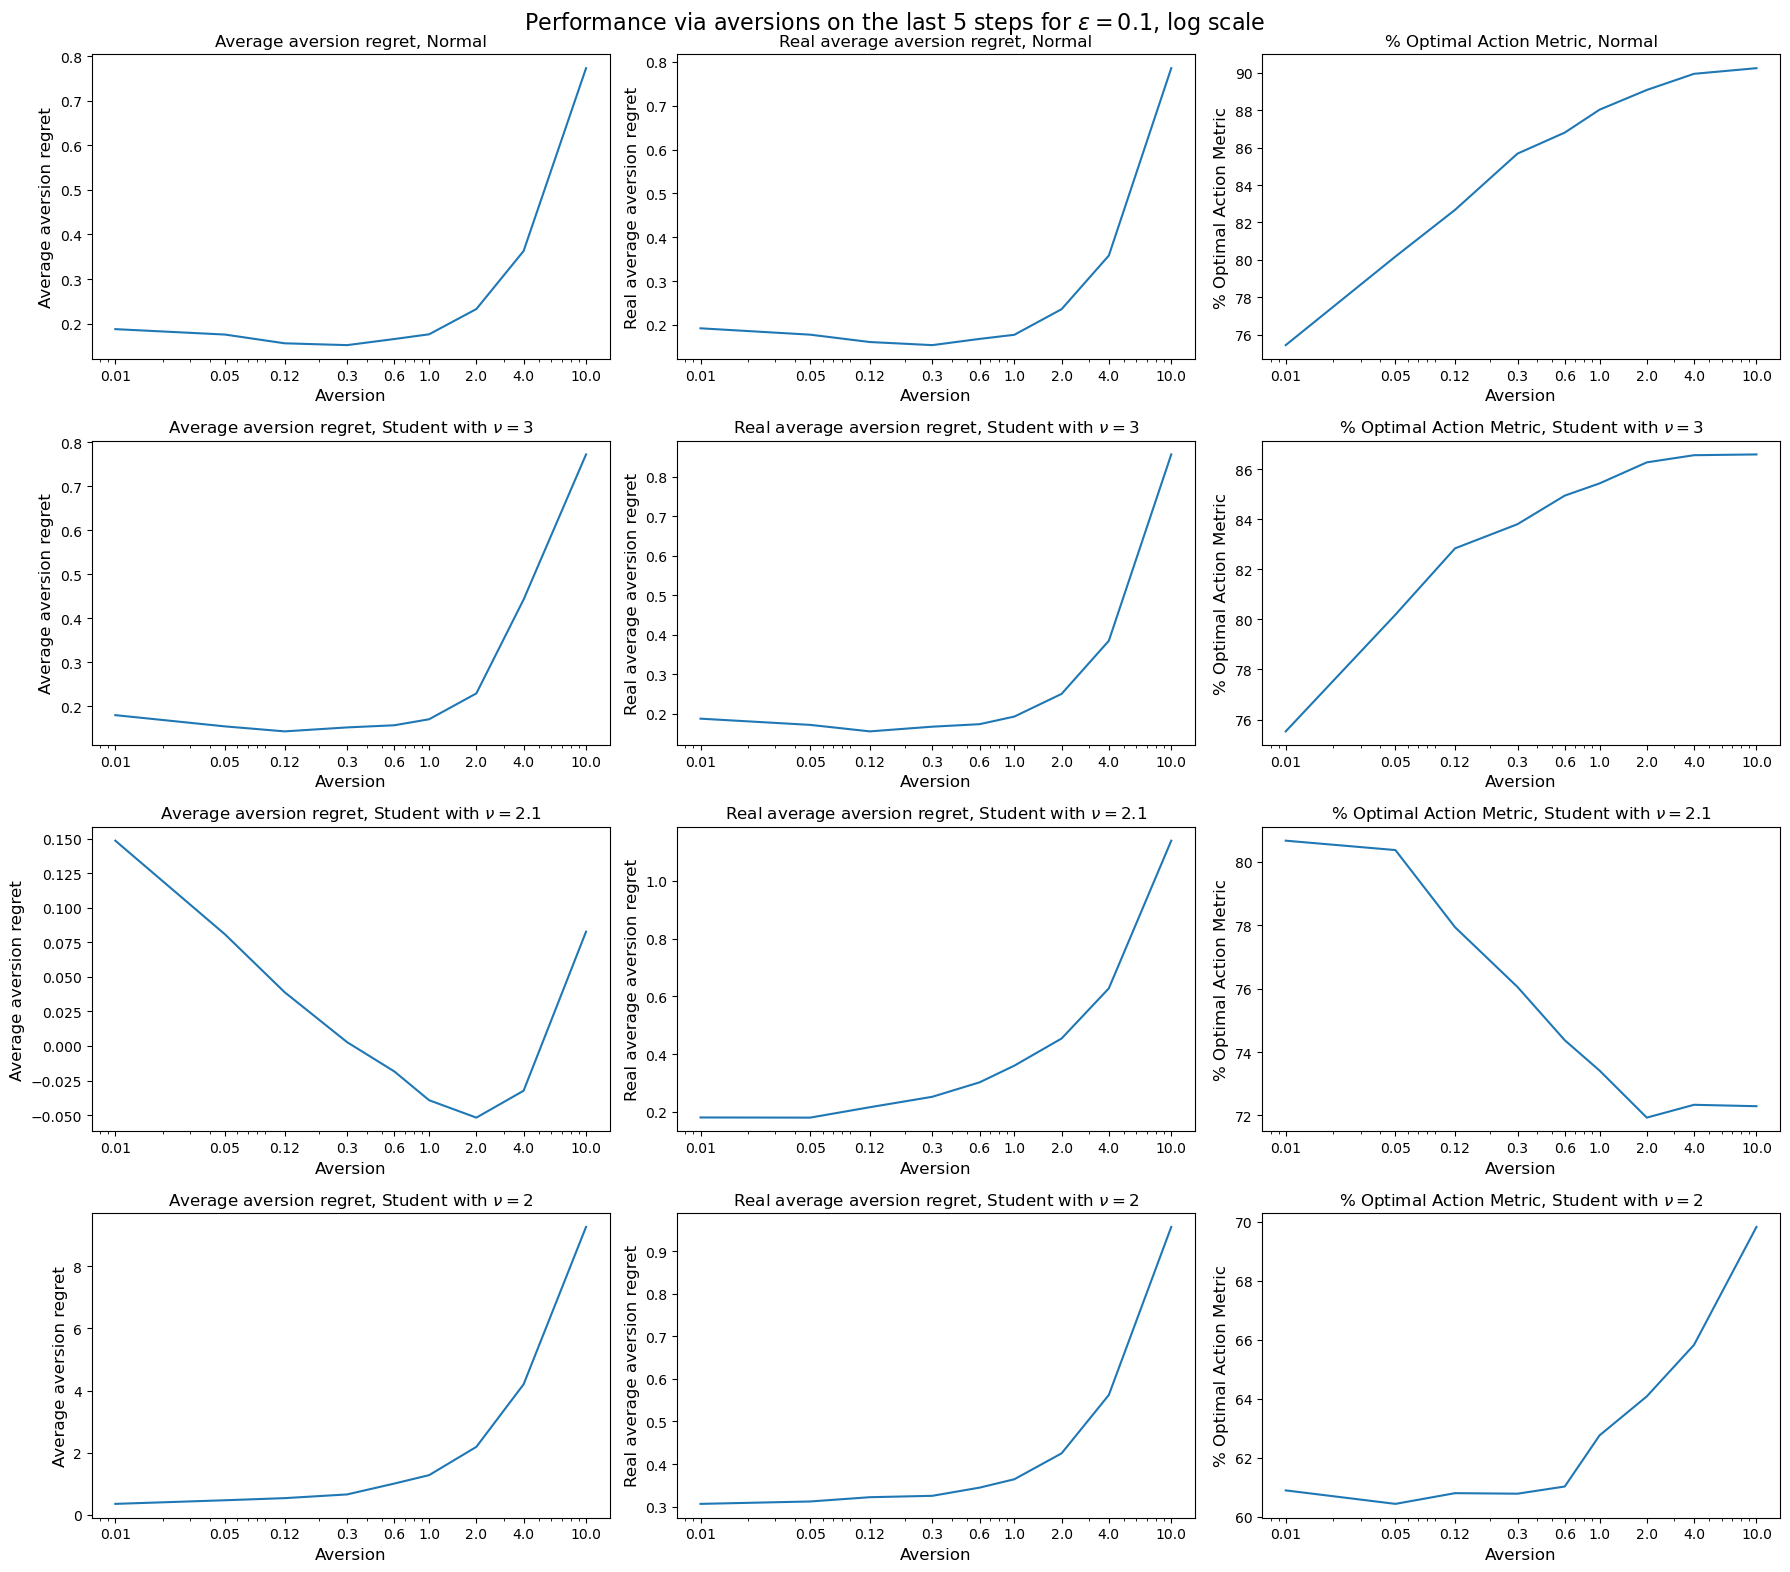
\includegraphics[width=6in]{experiments_aversion/eps_greedy/x_axis_aversion.png}
\caption{Графики зависимости метрик от количества шагов для каждого коэффициента отвращения.}
\label{fig:eps_greedy_aversion_selected_aversions}
\end{figure}

Что еще интересно, так это то, что при маленьком $\lambda$ эффективность для $t_{2.1}$ выше, чем для $t_3$ и $t_{\infty}$, но при увеличении коэффициента отвращения ситуация меняется, и  для $t_{2.1}$ метрики становятся хуже, чем для $t_3$ и $t_{\infty}$ (см. \ref{fig:eps_greedy_aversion_selected_aversions}). При больших $\lambda$, как было замечено выше, это связано с недооценкой дисперсии. При маленьких $\lambda$ дисперсия уже не играет при нахождении вероятностей никакой роли. Так в чем же дело? Стоит предположить, что дело в более остром пике у $t_{2.1}$: при нажатии на рычаг у $t_{2.1}$ выборочное матожидание ближе к настоящему матожиданию, чем у $t_3$ и $t_{\infty}$, что приводит к большей точности. Сама возможность приближения гарантируется числом $\epsilon$. Похожие рассуждения были приведены в параграфе \ref{subsec:classic_epsilon_greedy} про $\epsilon$-greedy стратегии в классической задаче о многоруких бандитах.

\subsection{Коррекция выборочной дисперсии}\label{sec:correction_eps_greedy}

Итак, как мы выяснили, в связи со смещенной влево (относительно матожидания) медианой у выборочного среднего $s_n^2$ алгоритм в большинстве случаев недооценивает реальную дисперсию распределения. Предположим, что алгоритму откуда-то стало известно семейство распределений, откуда генерируются активы. Модифицируем алгоритм, чтобы исправить описанную проблему.

Пусть алгоритм будет домножать выборочную дисперсию каждого распределения на определенную константу. Мы хотим домножить на такое число, чтобы произведение с большой вероятностью было близко к реальной дисперсии. Понятно, что при увеличении дисперсии в $\alpha$ раз распределение выборочной дисперсии тоже ``растягивается'' в $\alpha$ раз. Рассмотрим единичную дисперсию. Возьмем такие 2 варианта константы:
\begin{enumerate}
    \item $c_m = \frac{1}{m}$, где $m$ -- медиана распределения выборочной дисперсии $s_{1000}^2$ распределения с дисперсией $\sigma^2=1$ -- median correction.
    \item $c_{\mu} = \frac{1}{\mu}$, где $\mu$ -- мода распределения выборочной дисперсии $s_{1000}^2$ распределения с дисперсией $\sigma^2=1$ -- mode correction.
\end{enumerate}
Обе константы можно посчитать, сгенерировав $k$ выборок из $1000$ наград, где $k$ достаточно большое, посчитав в каждой выборке выборочную дисперсию, а затем среди полученных $k$ значений либо взять медиану, либо, взяв дискретизацию значений, посчитать среди них наиболее часто встречающееся. Взяв $k=5\cdot 10^{5}$ и дискретизацию по трем знакам после запятой, для $t_{2.1}$ были получены следующие значения: $c_m = 3.37269, \: c_{\mu} = 4.03226$. Подставим эти значения в алгоритм $\epsilon$-greedy с $\epsilon = 0.1$ и распределением $t_{2.1}$. При подсчете сожаления будем подставлять исправленную выборочную дисперсию. Сравним полученный результат с $0.1$-greedy алгоритмом без корректировки дисперсии.

\begin{figure}[ht!] %!t
\centering
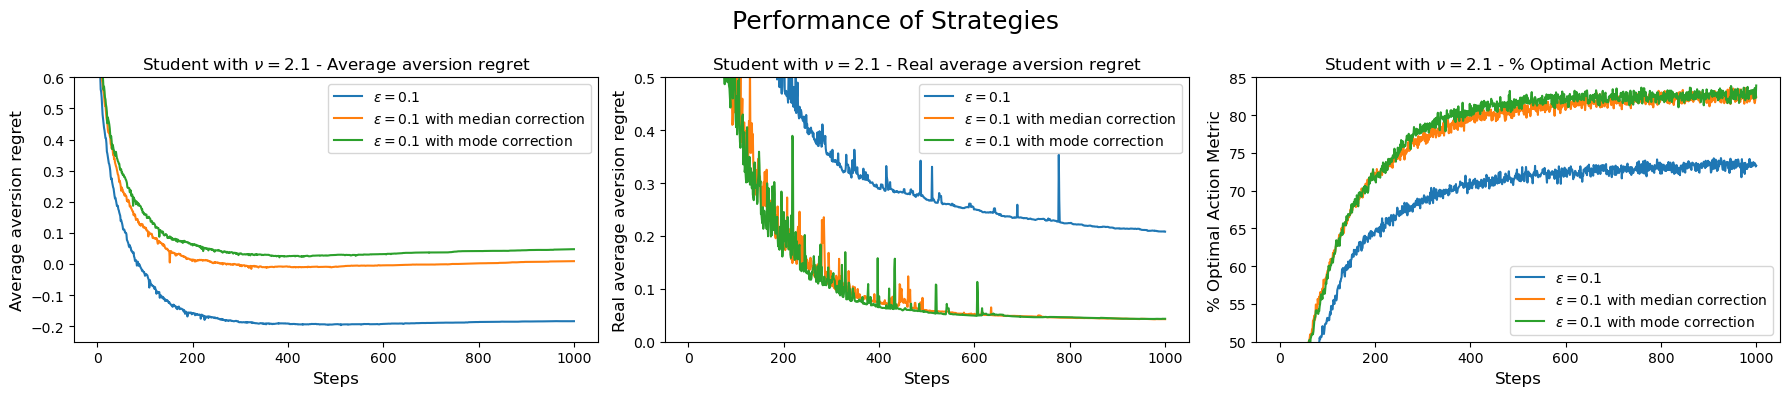
\includegraphics[width=6in]{theory_tester/theory_images/correction_variance/strat_distr.png}
\caption{Графики зависимости метрик от количества шагов для $t_{2.1}$ и стратегий с корректировкой выборочной дисперсии. Рассмотрена корректировка с помощью домножения на $c_m, \: c_{\mu}$ и без домножения (обычный $\epsilon$-greedy)}
\label{fig:aversion_correction_aversion_strat_distr}
\end{figure}

\begin{figure}[ht!] %!t
\centering
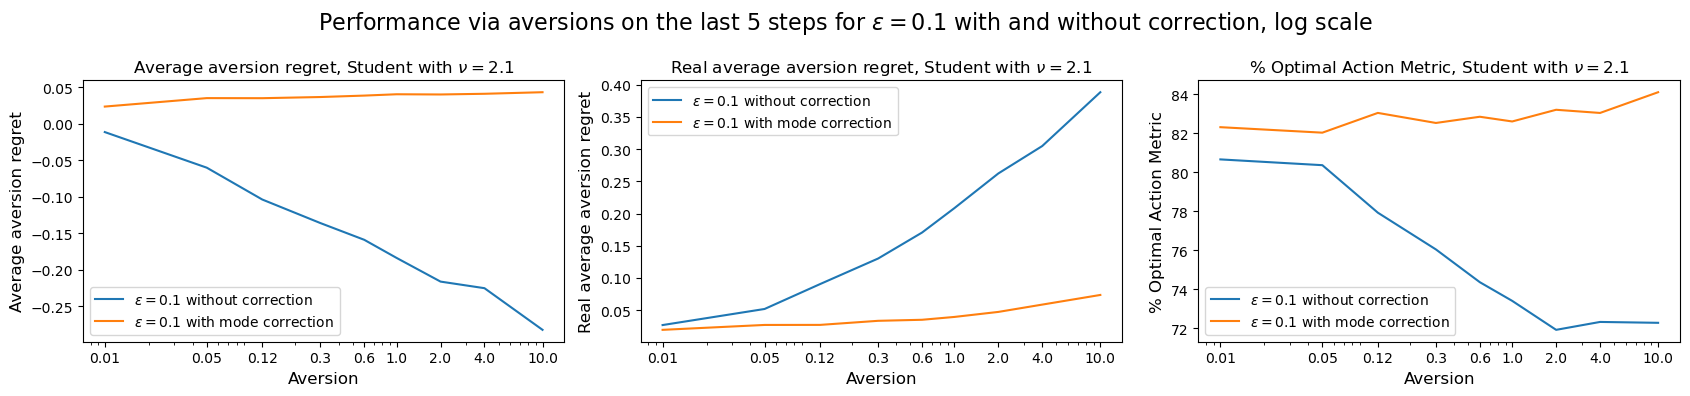
\includegraphics[width=6in]{theory_tester/theory_images/correction_variance/aversions_last_5_steps.png}
\caption{Графики зависимости метрик от коэффициента отвращения для $t_{2.1}$ и стратегий с корректировкой выборочной дисперсии. Рассмотрена корректировка с помощью домножения на $c_{\mu}$ и без домножения (обычный $\epsilon$-greedy)}
\label{fig:aversion_correction_last_5_steps}
\end{figure}

Как можно видеть, коррекция дисперсии значительно улучшает значения метрик. В частности, метрика Regret для стратегий с увеличением дисперсий не опускается ниже 0. Но процент оптимальных действий достигает максимального значения в примерно $85\%$, что меньше $90\%$, то есть у этих стратегий, при всех их преимуществах, устранены не все недостатки. Хотя у коррекций с помощью медианы и моды примерно одинаковые результаты, последняя все-таки незначительно лучше.

Оценим изменение значения метрик при различных коэффициентах отвращения для обычной $0.1$-greedy стратегии и для $0.1$-greedy стратегии с коррекцией с помощью моды.

Увеличение выборочной дисперсии практически устраняет с увеличением $\lambda$ ухудшение метрик Regret и Regret$_{\text{real}}$ и полностью устраняет уменьшение процента оптимальных действий. При этом в случае с процентом оптимальных действий можно наблюдать некоторое уменьшение метрик при $\lambda \to 0$, то есть начинает проявляться эффект неточности для двух рычагов с наибольшим матожмданием. В случае же Regret полномтью пропала переоценка стратегией самой себя. В целом же значения метрик для коррекции с помощью $c_{\mu}$ лучше, чем без коррекции при всех $\lambda$.

Хотя домножение дисперсии значительно улучшает эффективность стратегии, в реальной жизни это малоприменимо -- зачастую нам неизвестно число степеней свободы у распределения прибыли актива. Угадать константу, на которую нужно домножить, тоже не представляется возможным, поскольку значение медианы при $\nu > 2$ меняется от 0 до 1, и поэтому $c_m$ (и $c_{\mu}$) меняются от 1 до $\infty$ (см. \ref{fig:median_depend_on_df}).

\subsection{Адаптивный $\epsilon$-greedy}

Вернемся к стратегиям без коррекции дисперсии. Для стратегий с адаптивным $\epsilon$ получились следующие результаты (см. \ref{fig:adaptive_eps_strat_distr}):

Для всех распределений наилучшие результаты показали стратегии с начальным $\epsilon=10$. Это объясняется тем, что на начальных шагах у этих стратегий происходит фаза exploration, во время которой вероятности нажатий на рычаги распределены почти равномерно. Из-за этого дисперсии и матожидания приближаются более точно. Для $t_3$ и $t_{\infty}$ наилучший результат показала адаптивная $\epsilon$-greedy стратегия с $\epsilon=10$. Чуть хуже результаты у VDBE с $\epsilon=10$. Для $t_{2.1}$ эти стратегии показали примерно одинаковый результат. В отличие от $\epsilon$-greedy, адаптивные стратегии склонны к сильной переоценке своих результатов на начальных шагах (в то время как $\epsilon$-greedy, наоборот, недооценивает себя).

\begin{figure}[ht!] %!t
\centering
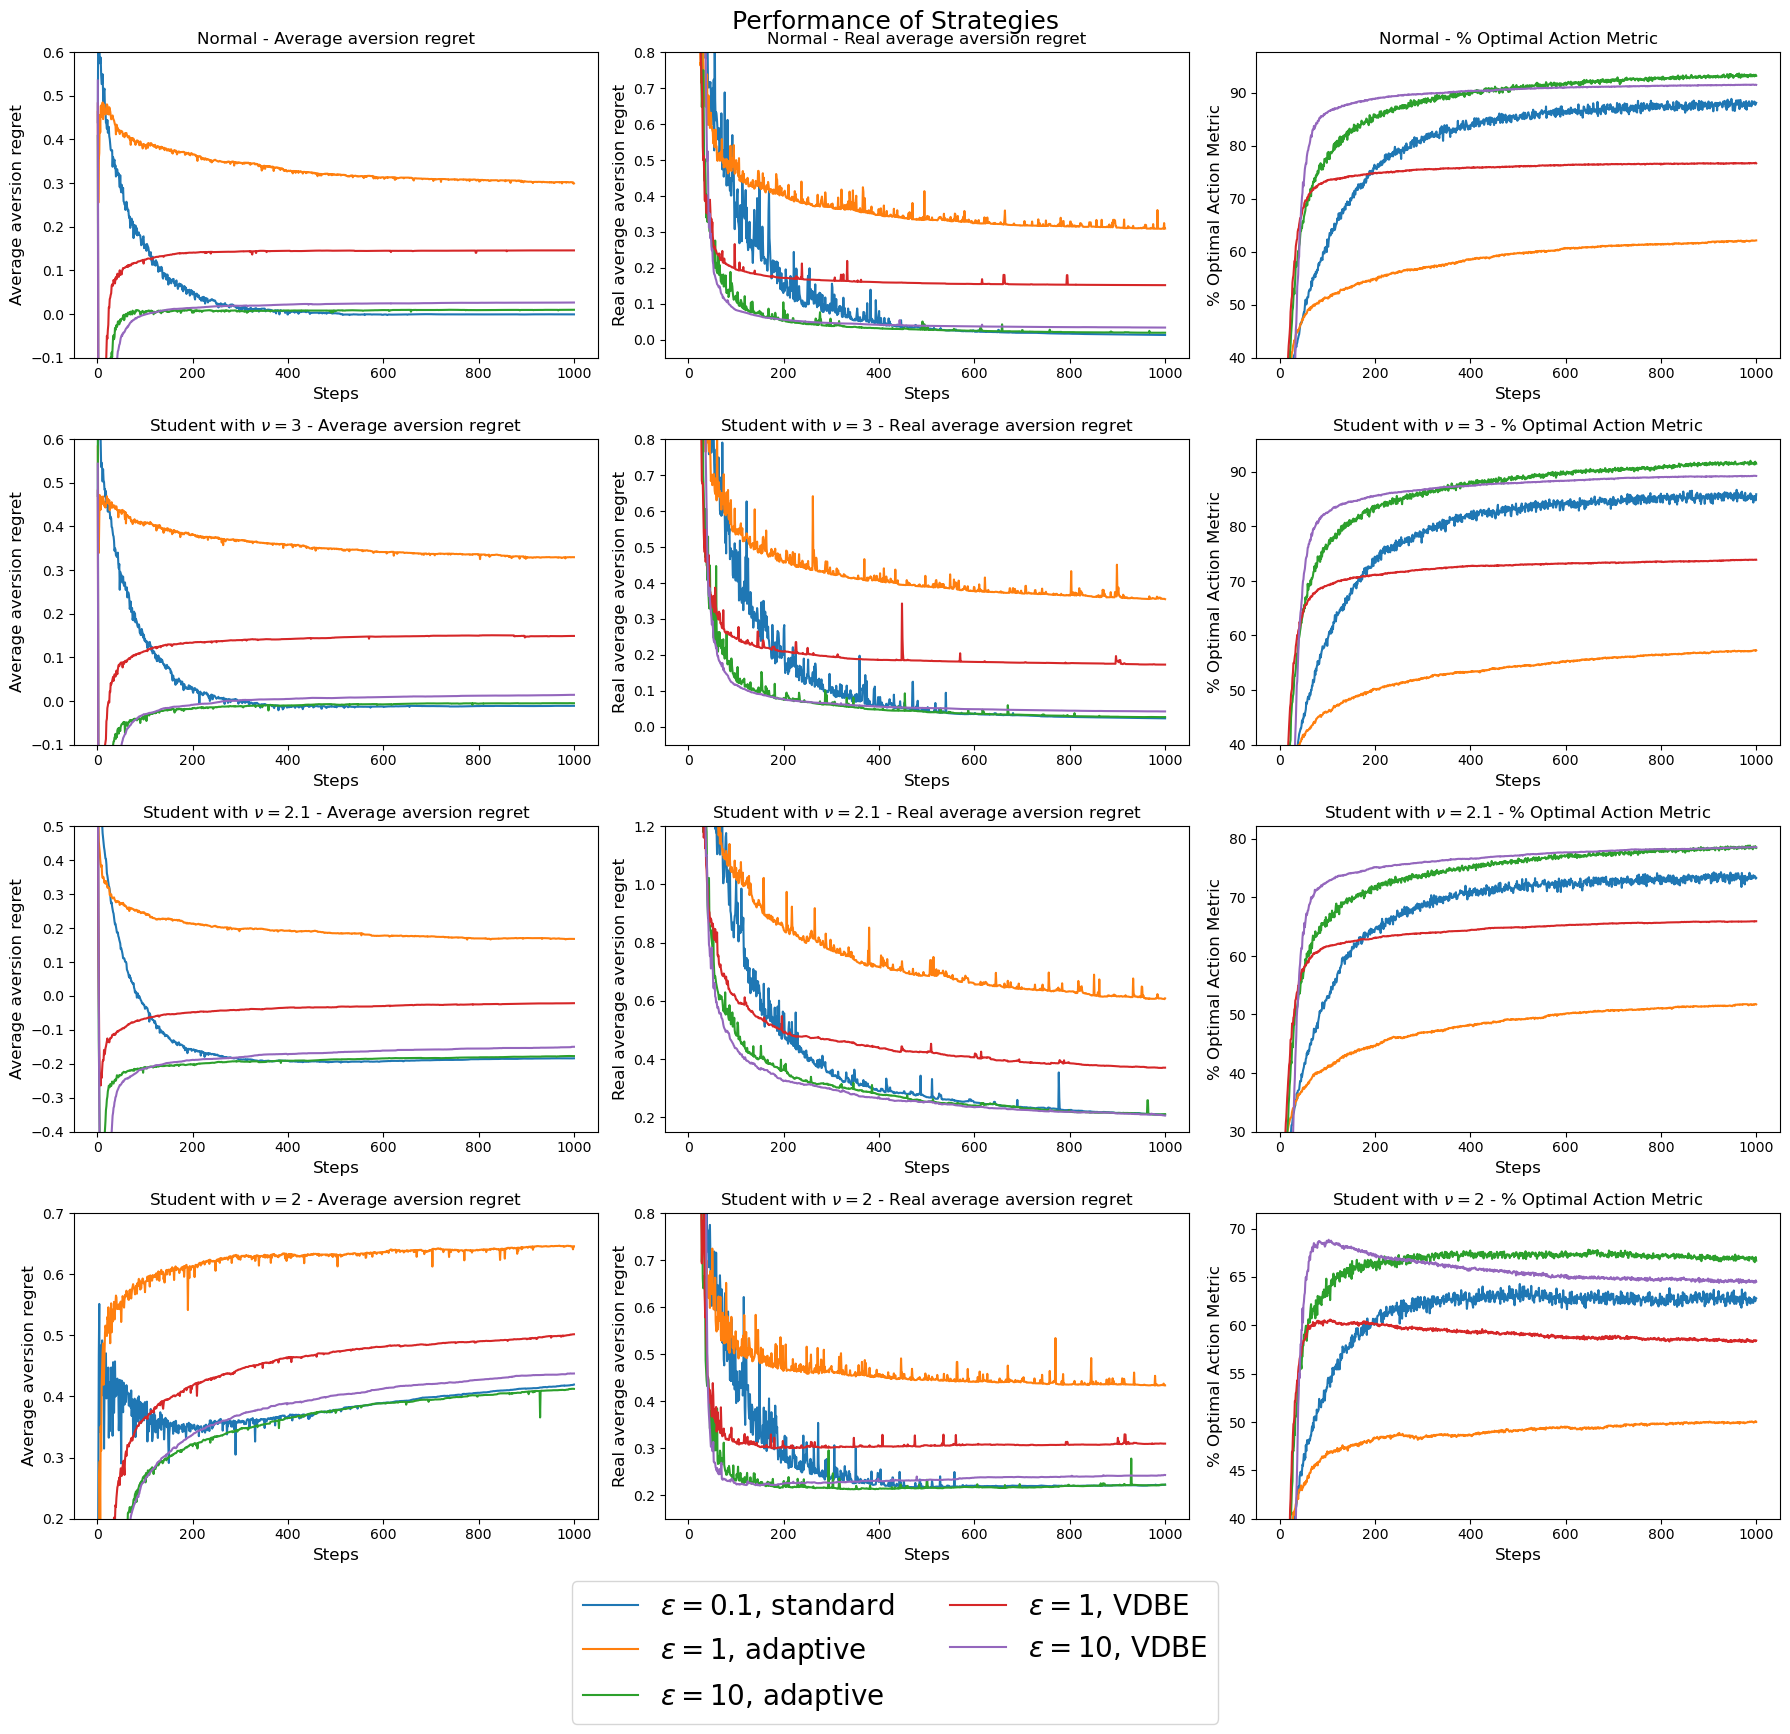
\includegraphics[width=6in]{theory_tester/theory_images/adaptive_epsilon/one_distr.png}
\caption{Зависимость метрик от количества шагов при $0.1$-greedy, adaptive-$\epsilon$ и VDBE стратегиях для различных распределений}
\label{fig:adaptive_eps_strat_distr}
\end{figure}

Поскольку стратегии с $\epsilon=10$ показали наилучший результат, посмотрим на изменение метрик для этих стратегий при различных коэффициентах отвращения:

\begin{figure}[ht!] %!t
\centering
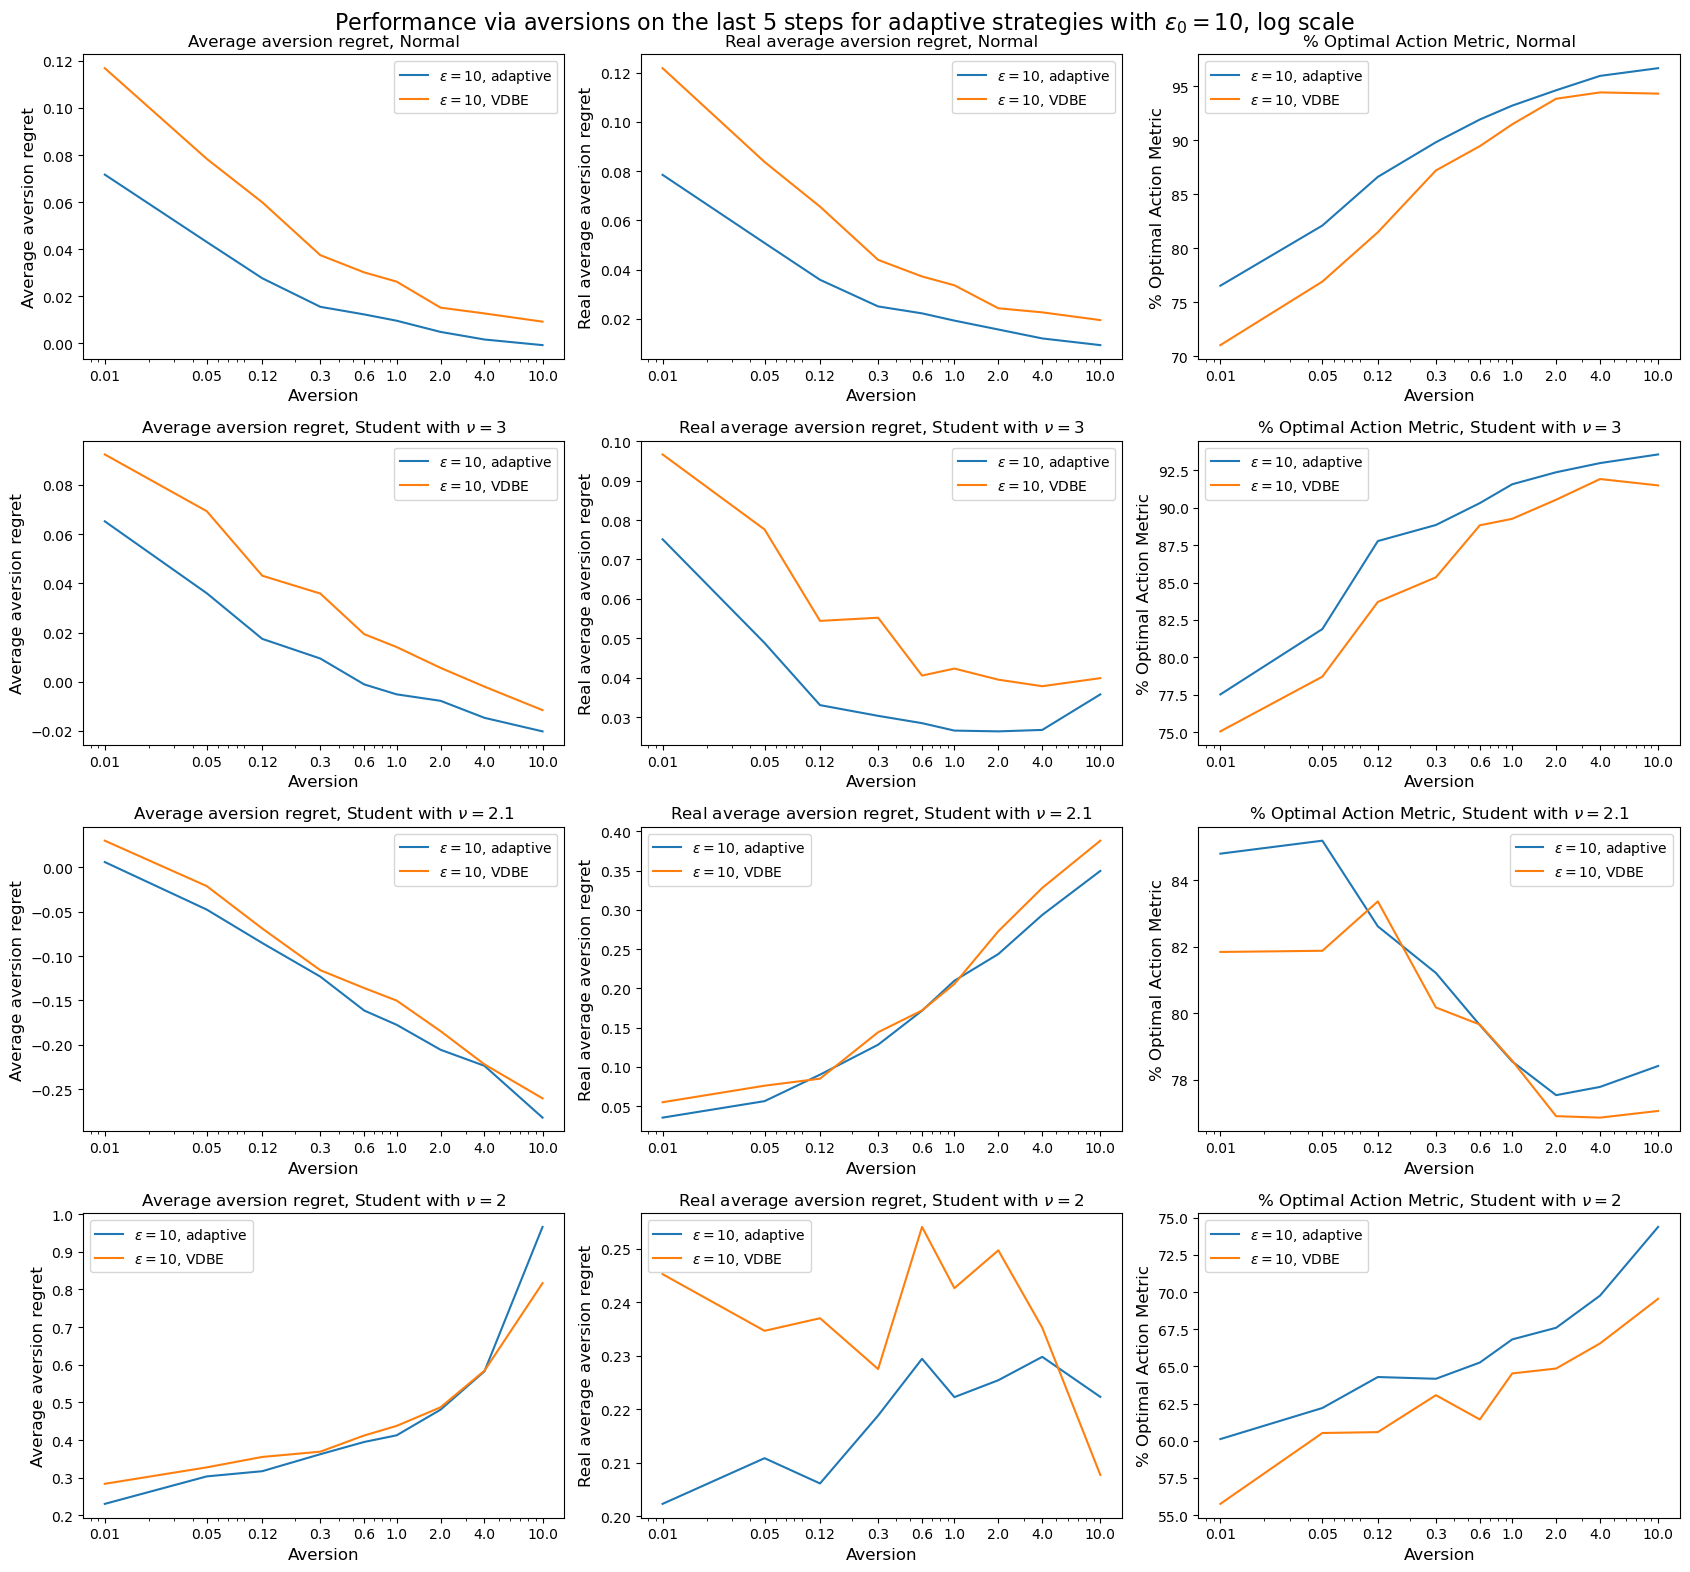
\includegraphics[width=6in]{theory_tester/theory_images/adaptive_epsilon/aversion_last_5_steps.png}
\caption{Графики зависимости метрик от коэффициента отвращения для $t_{2.1}$ и стратегий adaptive-$\epsilon$ и VDBE с $\epsilon=10$.}
\label{fig:adaptive_eps_last_5_steps}
\end{figure}

Как видно из \ref{fig:adaptive_eps_last_5_steps}, тенденция изменения метрик с изменением $\lambda$ схожа с таковой у $\epsilon$-greedy стратегии. Также стратегия adaptive-$\epsilon$ показывает себя лучше, чем VDBE. Однако VDBE обладает бОльшим потенциалом, поскольку позволяет настраивать дополнительные параметры -- температуру $\tau$ и шаг обновления $\delta$. Изучение поведения VDBE при различных параметрах $\epsilon$, $\tau$ и $\delta$ может быть интересной темой для дальнейших исследований.

\subsection{Позитивная инициализация}

Как было замечено ранее, для $t_{\nu}$ с $\nu > 2$ в обычной задаче о многоруких бандитах позитивная инициализация с постоянным step-size показывает результат лучше, чем $\epsilon$-greedy, при этом обучаясь до наибольших значений своих метрик за горяздо меньшее время. При этом у позитивной инициализации наблюдался эффект переобучения. Попробуем посмотреть на результаты этой стратегии в задаче с присутствием неприятия к риску.

\begin{figure}[ht!] %!t
\centering
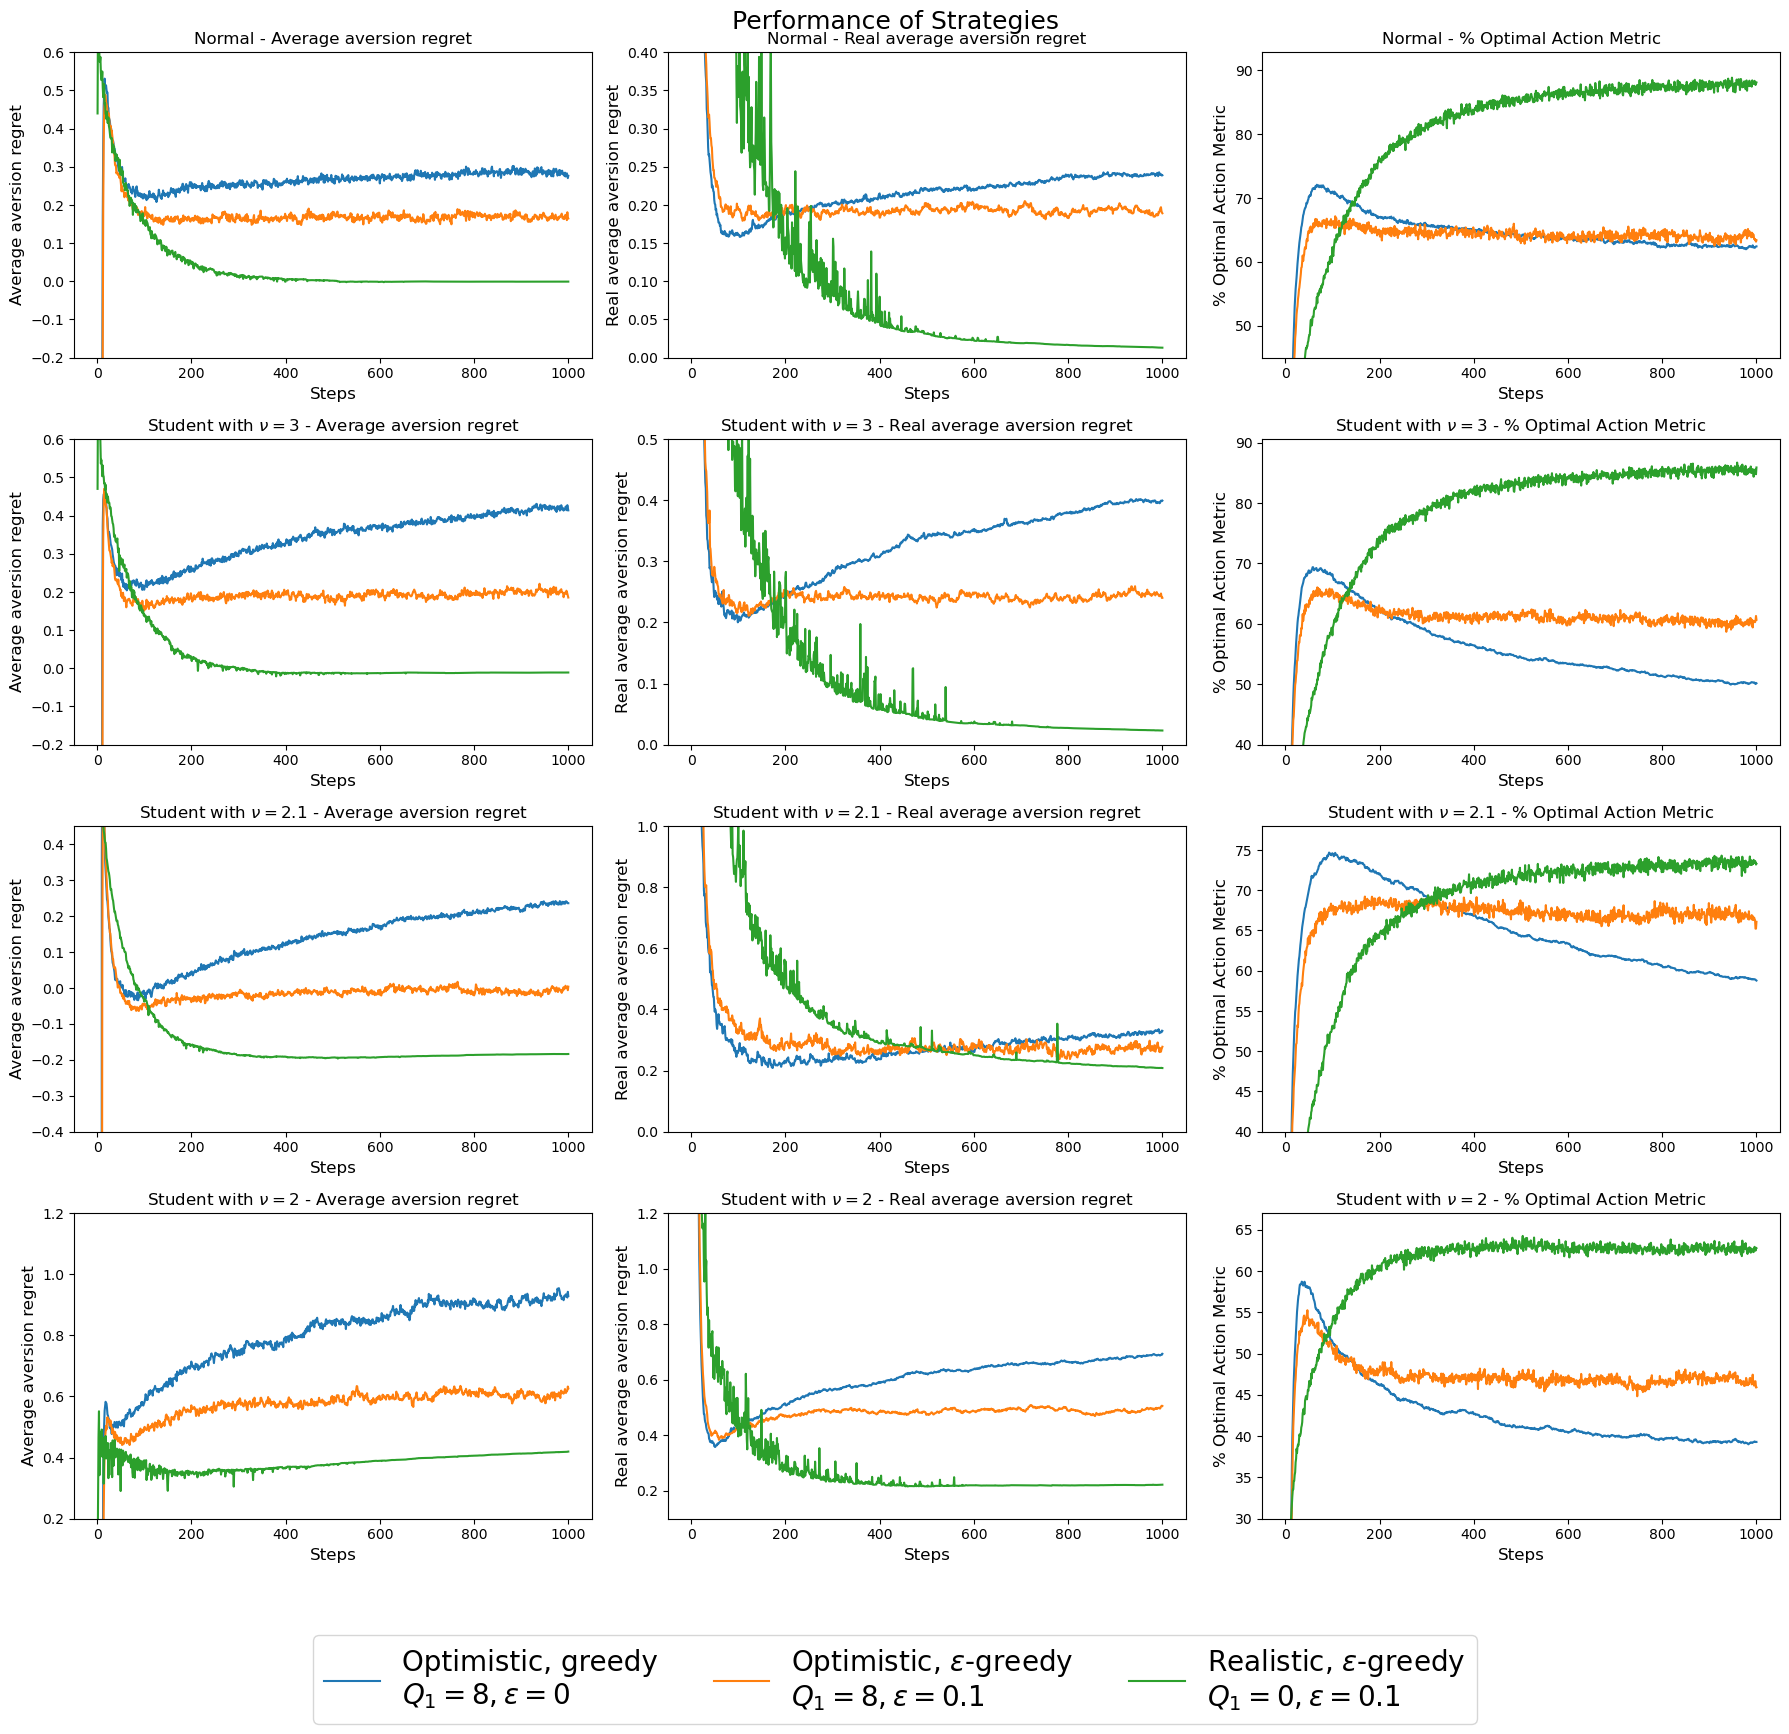
\includegraphics[width=6in]{theory_tester/theory_images/positive_init/one_distr.png}
\caption{Зависимость метрик для различных распределений от количества шагов при стратегиях с позитивной инициализацией, постоянным step-size и $\epsilon=0$ или $\epsilon=0.1$, а также при $0.1$-greedy стратегии}
\label{fig:positive_init_one_distr}
\end{figure}

Так же, как и в обычной задаче о многоруких бандитах, при позитивной инициализации наблюдается эффект переобучения. Однако в задаче о многоруких бандитах с учетом неприятия к риску эта стратегия превосходит $\epsilon$-greedy только для $t_{2.1}$. Несомненныи плюсом является то, что для достижения наилучших значений метрик позитивной инициализации понадобилось намного меньше шагов, чем $\epsilon$-greedy -- около 100 против 1000. Что еще интересно, так это то, что при $\lambda \to 2+$ наилучший процент оптимальных действий для жадной стратегии с позитивной инициализацией увеличивается (см. \ref{fig:positive_init_one_strat_positive_greedy}).

\begin{figure}[ht!] %!t
\centering
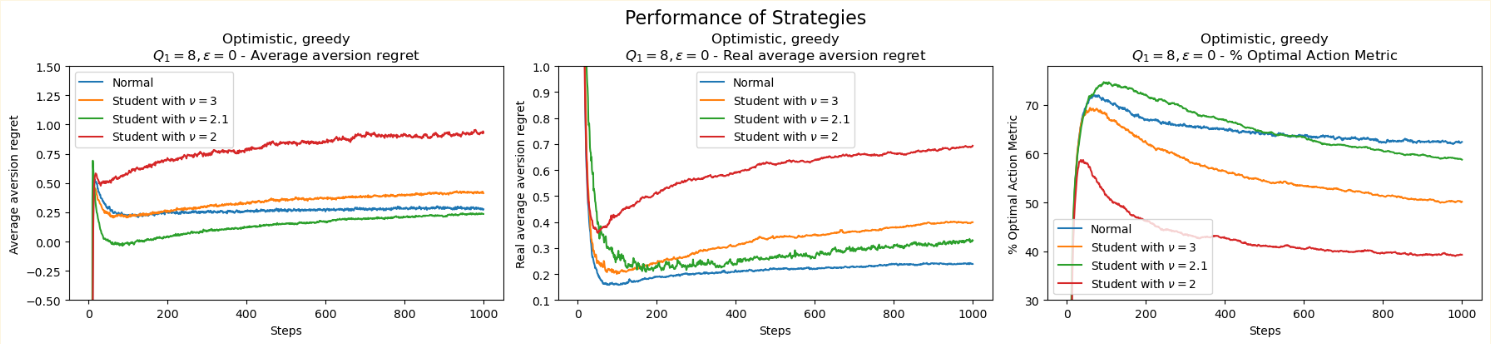
\includegraphics[width=6in]{theory_tester/theory_images/positive_init/one_strat_positive_greedy.png}
\caption{Зависимость метрик для различных распределений от количества шагов для жадной стратегии с позитивной инициализацией и постоянным step-size}
\label{fig:positive_init_one_strat_positive_greedy}
\end{figure}

\subsection{UCB}

В UCB изменению подверглось только выборочное матожидание, выборочную дисперсию изменения не тронули. Неудивительно, что UCB лишь незначительно улучшил результат для $t_{2.1}$, в остальных случаях показав ухудшение относително $0.1$-greedy (см. \ref{fig:ucb_compare_ucb_and_eps_greedy}).

\begin{figure}[ht!] %!t
\centering
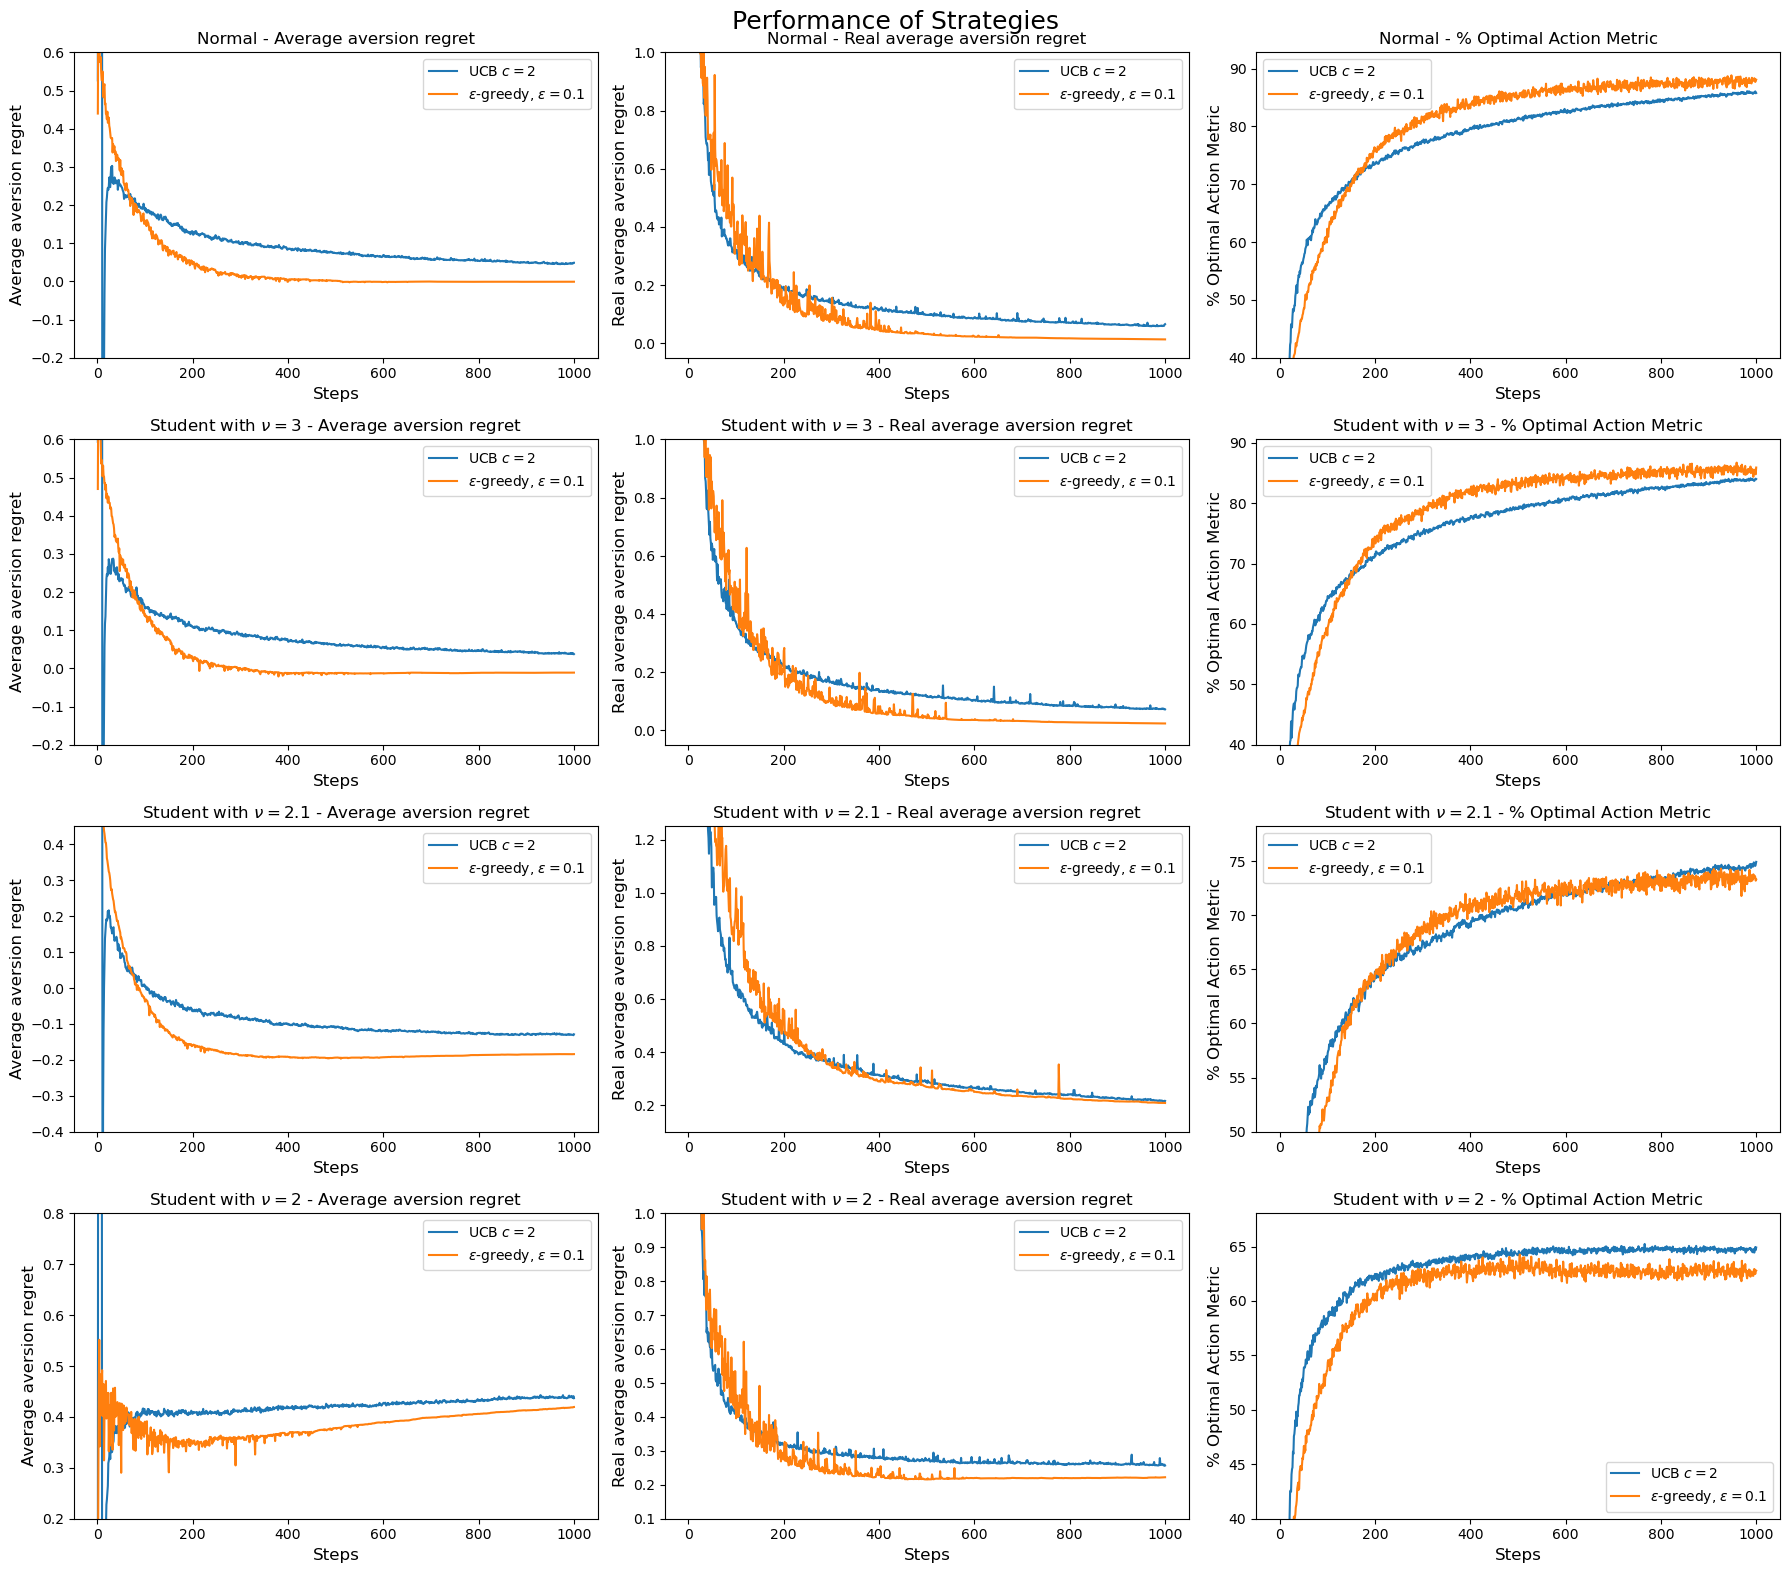
\includegraphics[width=6in]{theory_tester/theory_images/UCB/compare_ucb_and_eps_greedy.png}
\caption{Зависимость метрик для различных распределений от количества шагов для UCB с $c=2$ и $0.1$-greedy}
\label{fig:ucb_compare_ucb_and_eps_greedy}
\end{figure}

\begin{figure}[ht!] %!t
\centering
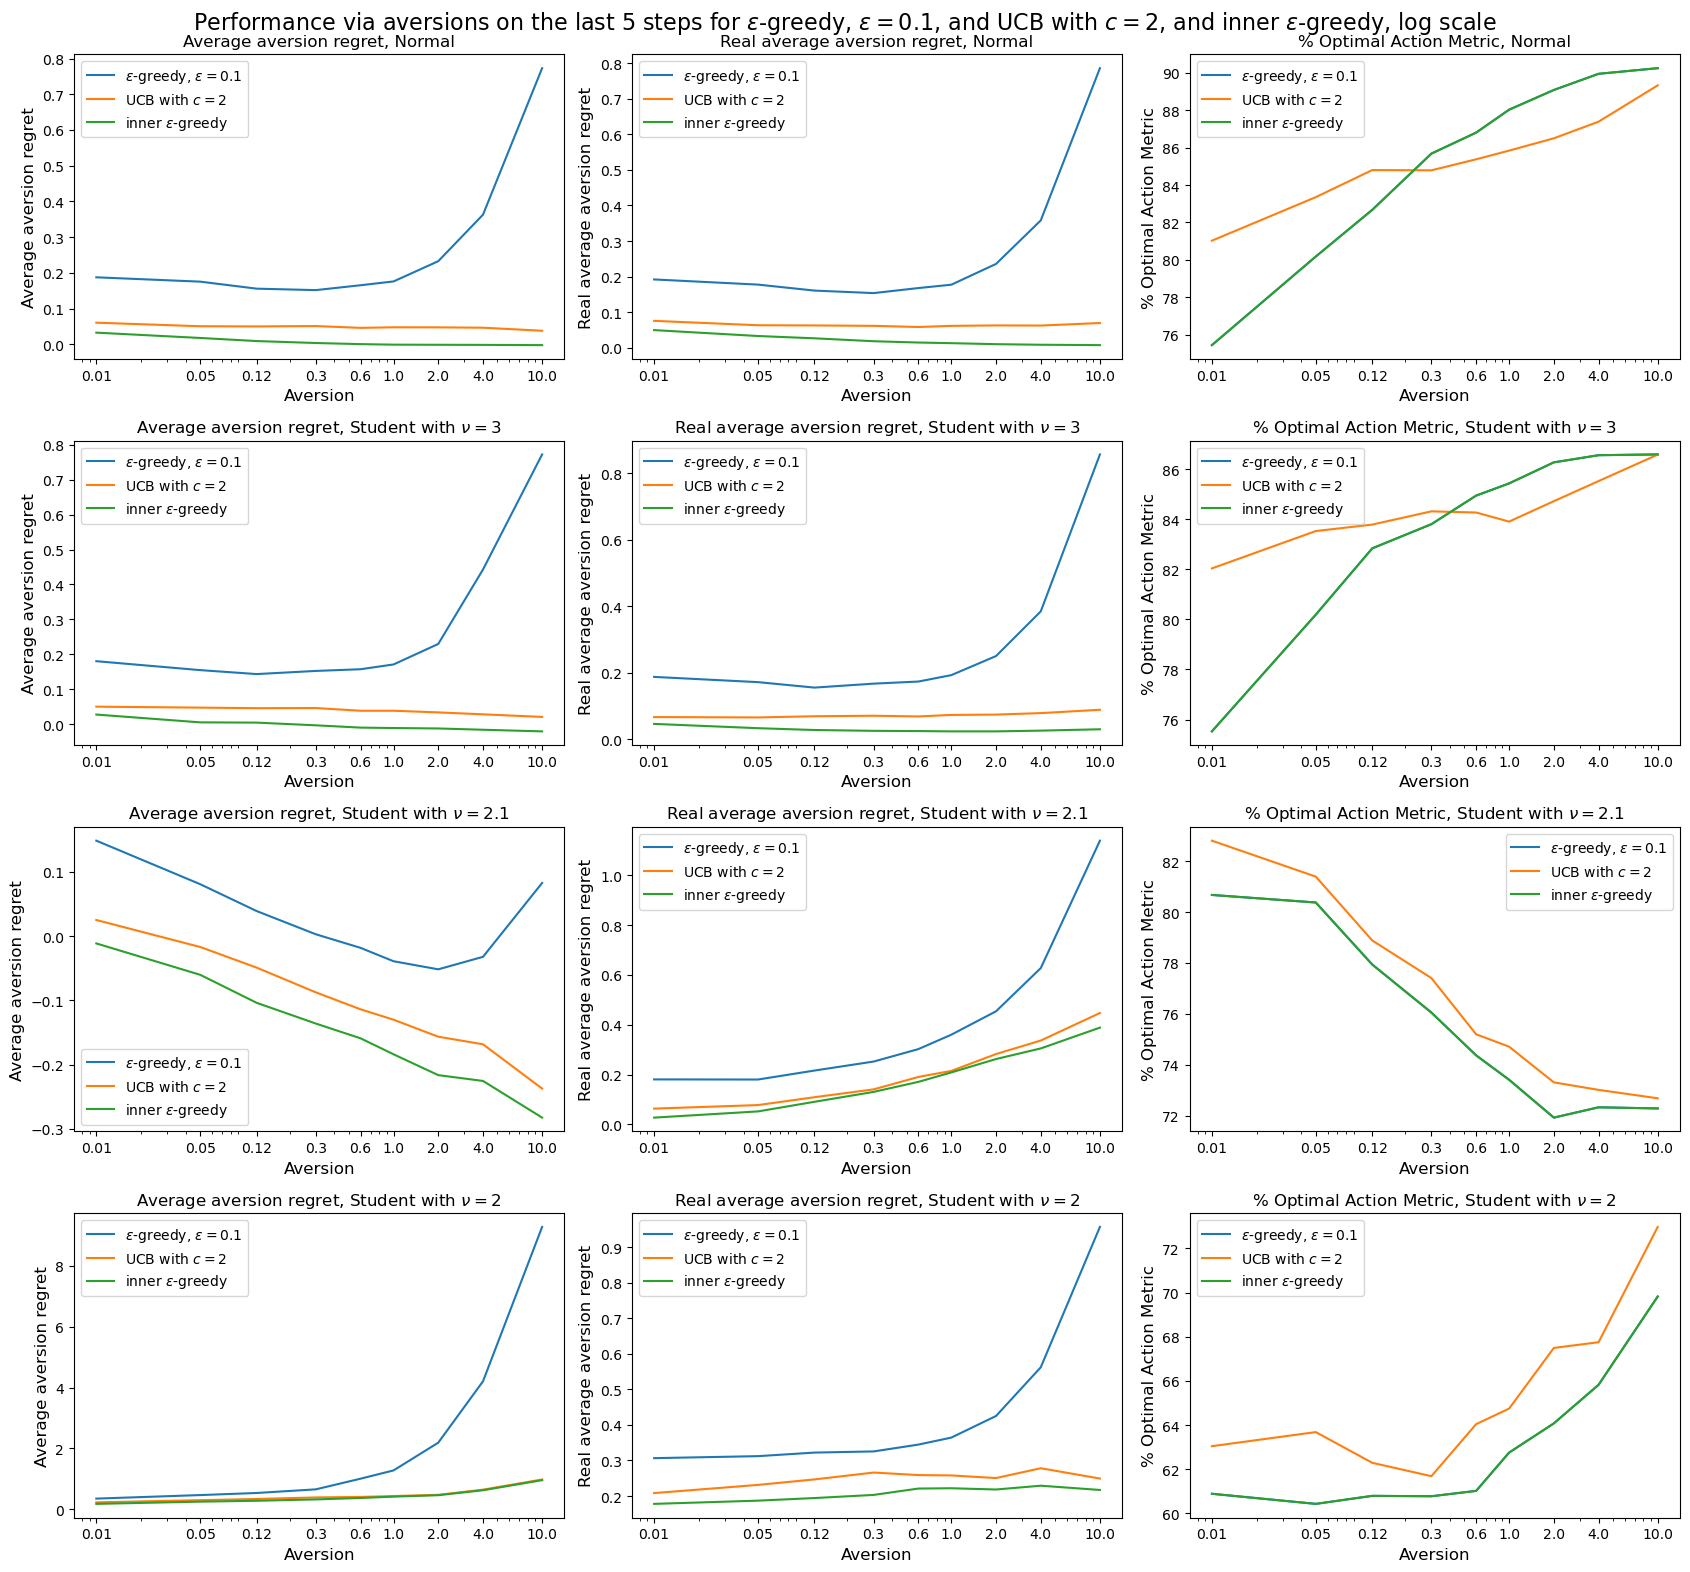
\includegraphics[width=6in]{Figures/experiments_aversion/ucb/last_5_steps.png}
\caption{Графики зависимости метрик от коэффициента отвращения для различных распределений и стратегий UCB с $c=2$, $\epsilon$-greedy и $\epsilon$-greedy с внутренней вероятностью}
\label{fig:ucb_compare_ucb_for_different_aversions}
\end{figure}

Однако, что интересно (\ref{fig:ucb_compare_ucb_for_different_aversions}), во-первых, для $t_{2.1}$ при любом $\lambda$ у UCB процент оптимальных действий выше, чем у $\epsilon$-greedy. Во-вторых, при маленьких $\lambda$ процент оптимальных действий у UCB выше, чем у $\epsilon$-greedy. Это объясняется тем, что прибавка вида $c\sqrt{\frac{\log t}{N_t(a)}}$ позволяет двум рычагам с наибольшими матожиданиями прожаться большее число раз, что дает лучшее приближение и, как следствие, лучший процент оптимальных действий. В-третьих, при всех $t_{\nu}$ и всех $\lambda$ значение метрики Regret$_{\text{real}}$ у UCB выше, чем у $\epsilon$-greedy (при том, что в некоторых случаях процент оптимальных действий лучше). После измерения дисперсий метрик оказалось, что дисперсии Regret$_{\text{real}}$ для UCB и $\epsilon$-greedy одинаковы. Такое странное поведение метрик можно объяснить большей рискованностью UCB: хотя UCB в среднем подбирается ближе к оптимальной точке, чем $\epsilon$-greedy, UCB подбирается к этой точке с более ``крутой'' стороны, что дает более сильное падение результата. По этой причине, хотя стратегия имеет право на существование, все же она не подходит для реальной жизни.

\subsection{Gradient bandits}

Как и в классической задаче о многоруких бандитах, добавление baseline существенно улучшает показания метрик (\ref{fig:aversion_gradient_check_strategies_by_distribution}):

\begin{figure}[ht!] %!t
\centering
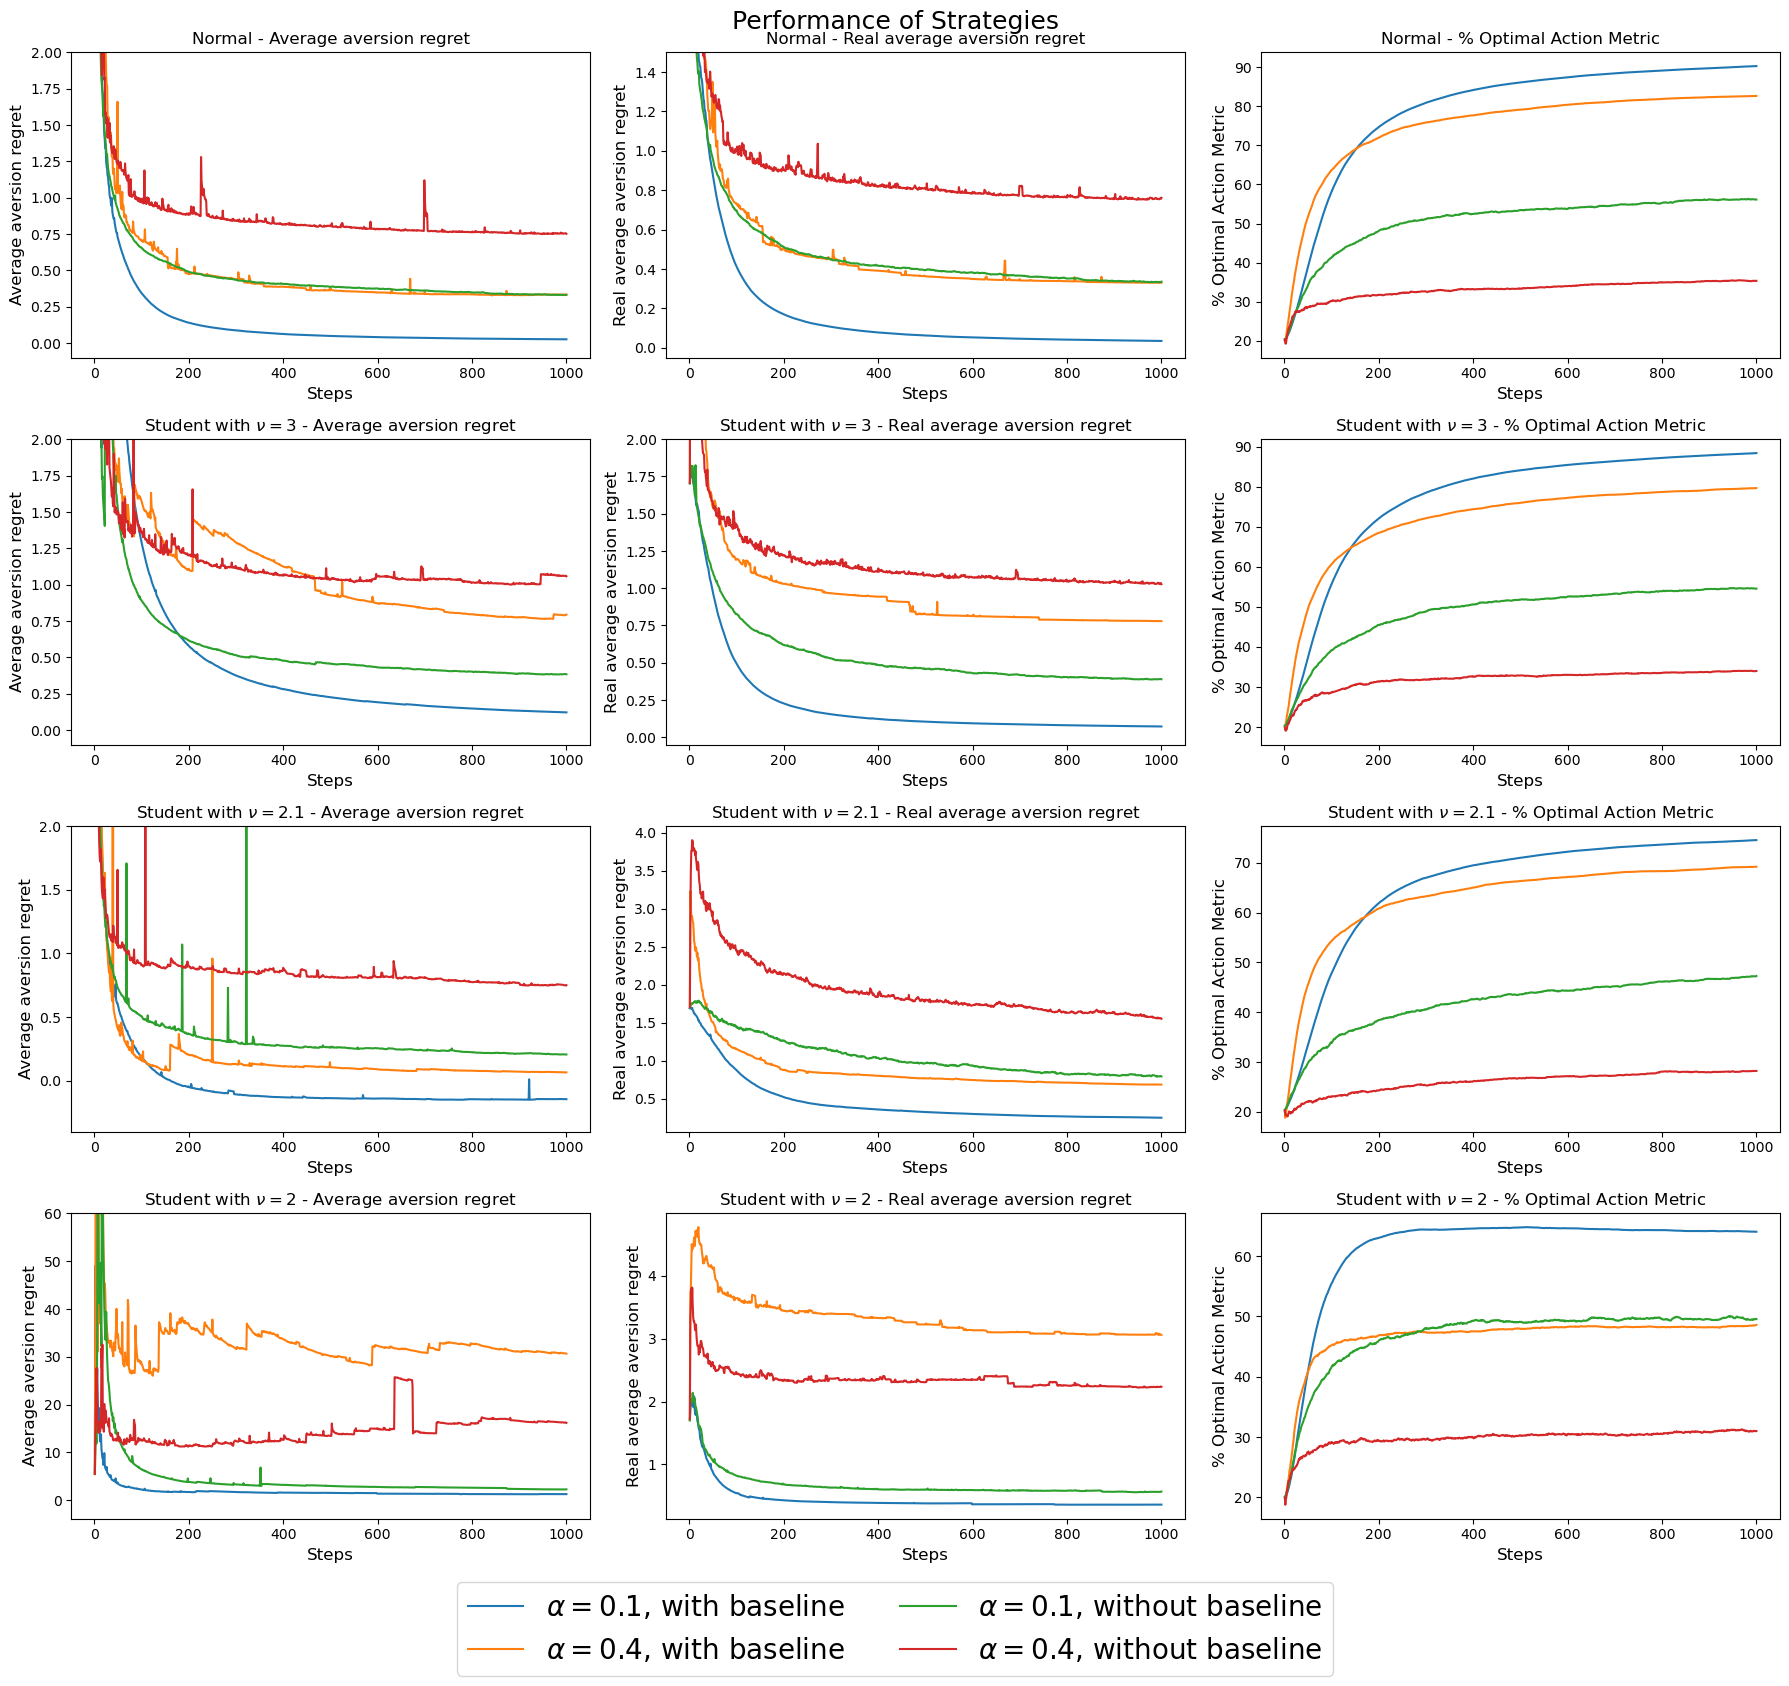
\includegraphics[width=6in]{Figures/experiments_aversion/gradient_bandits/check_strategies_by_distribution.png}
\caption{Графики зависимости метрик количества шагов для различных распределений и стратегий с градментных бандитов с разными baseline и $\alpha$ в измененной задаче}
\label{fig:aversion_gradient_check_strategies_by_distribution}
\end{figure}

Отличный результат для всех метрик показывает, что в теоретической главе был выбран удачный baseline. Результаты по коэффициентам отвращения даны в \ref{fig:aversion_gradient_bandits_last_5_steps}. Результаты улучшают вероятности для реального $\epsilon$-greedy и ухудшают для внутренних вероятностей $\epsilon$-greedy.

\begin{figure}[ht!] %!t
\centering
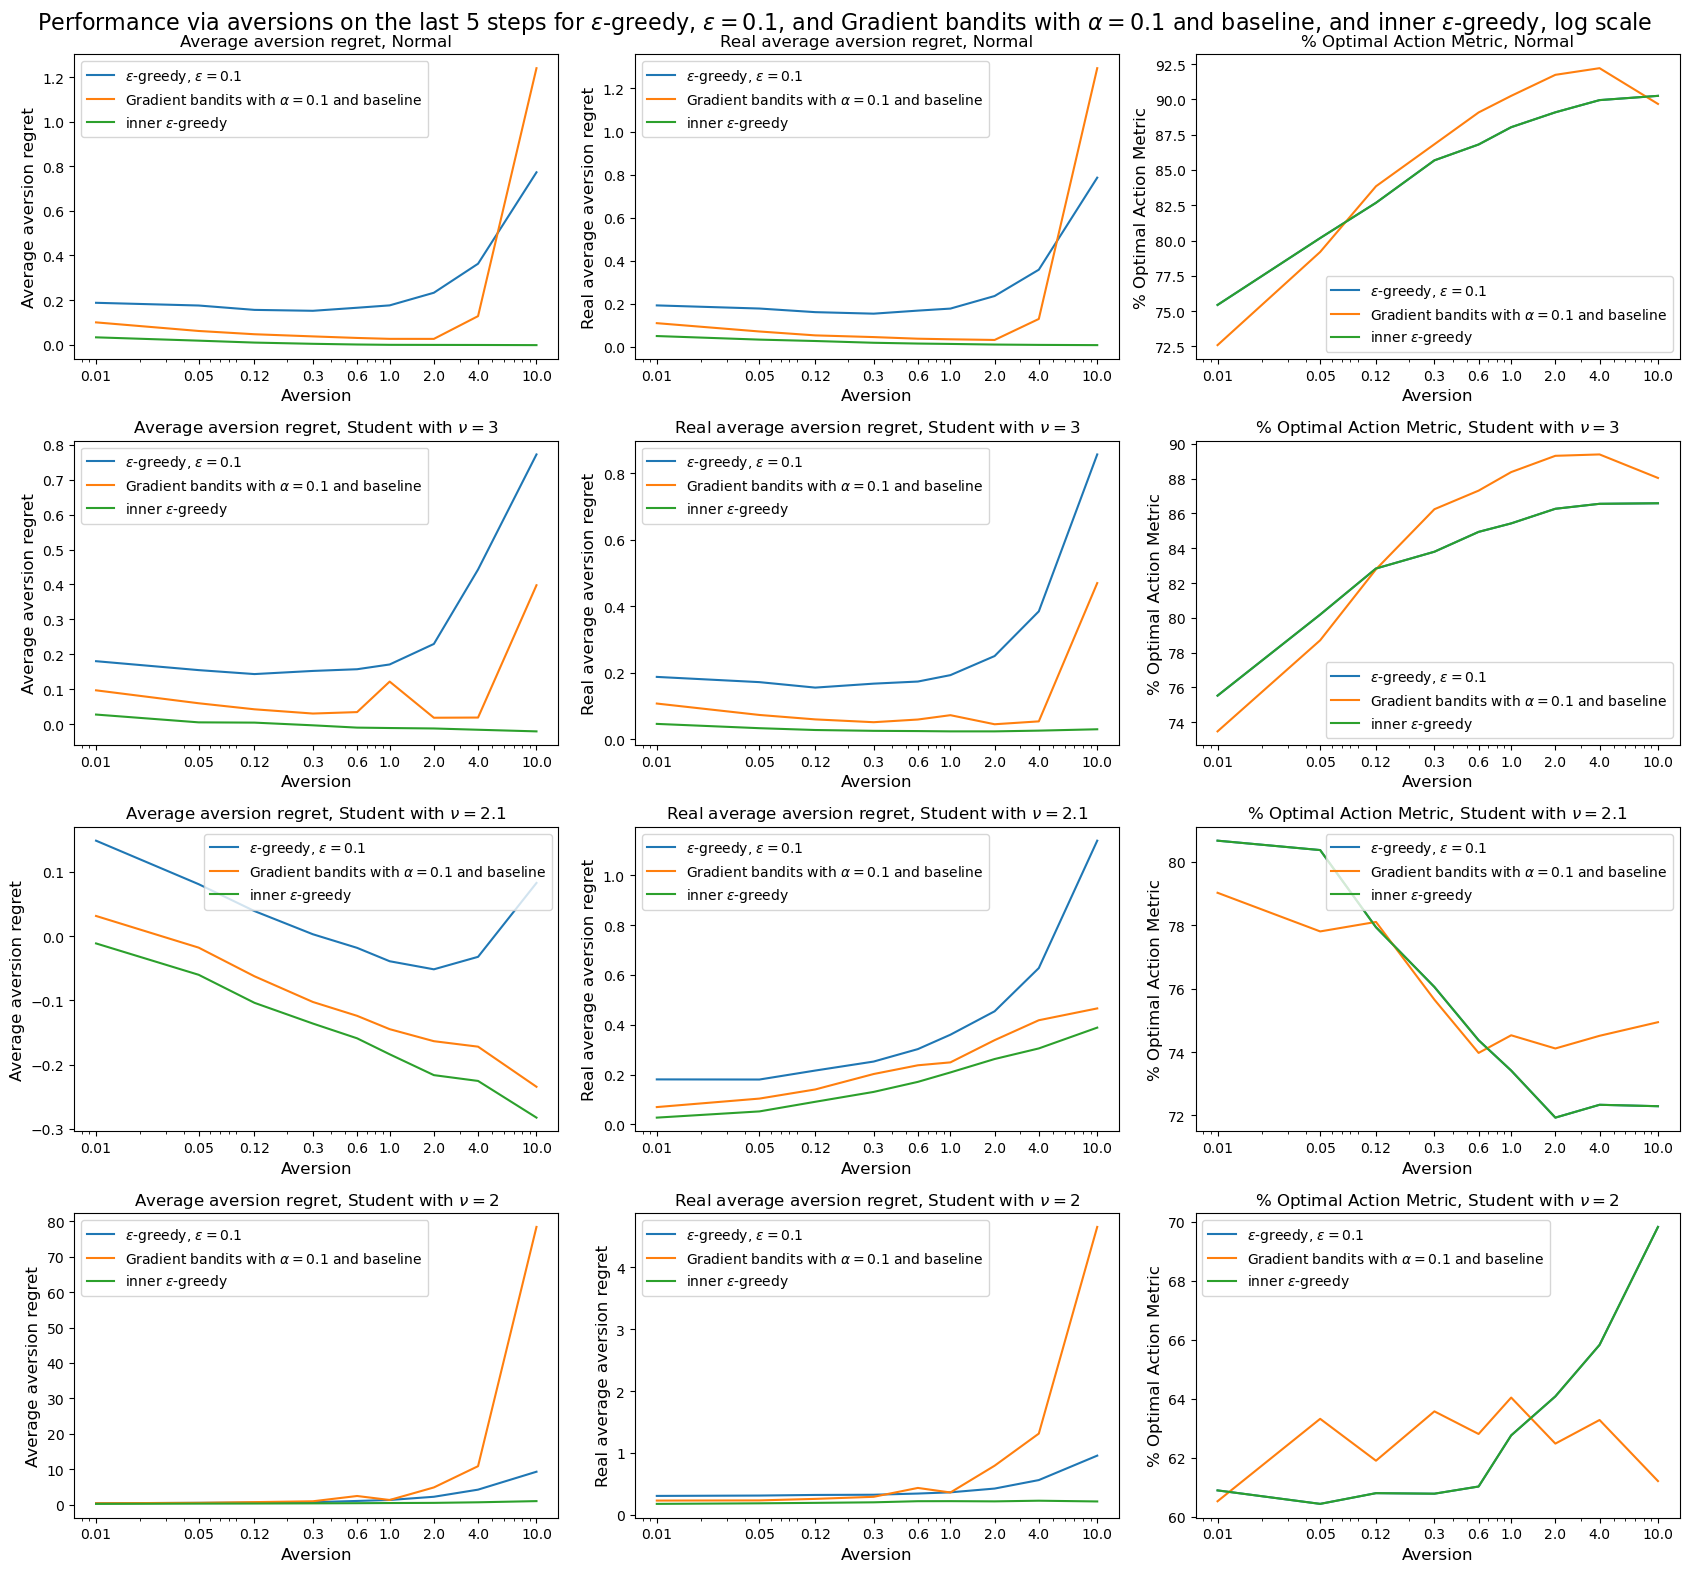
\includegraphics[width=6in]{Figures/experiments_aversion/gradient_bandits/last_5_steps.png}
\caption{Графики зависимости метрик от коэффициента отвращения для распределений и градиентных бандитов.}
\label{fig:aversion_gradient_bandits_last_5_steps}
\end{figure}


\section{Выводы}

По проведенным экспериментам можно сделать следующие выводы:
\begin{enumerate}
    \item Практически все стратегии справляются с достаточно маленькой ошибкой для распределений с большим числом степеней свободы, а именно $\nu \geq 3$
    \item Один из лучших результатов показала простая стратегия $\epsilon$-greedy. Несмотря на то, что внутри себя стратегия хранит вектор вероятностей, очень близко подходящий к оптимальному решению за 1000 шагов, в реальности с вероятностью $\epsilon$ будет выбираться случайный рычаг. Это повышает сожаление стратегии на $0.2$. Поэтому выбор стратегии $\epsilon$-greedy должен основываться на приоритетной цели: если необходимо получить наилучший вектор вероятностей, не считаясь с затратами при обучении, то $\epsilon$-greedy подходит. Если же важна эффективность и на обучении, то лучше рассмотреть другие стратегии, например, градиентных бандитов.
    \item Для $\epsilon$-greedy стратегии при $\nu \geq 3$ эффективность стратегий падает при $\lambda \to 0$. Это связано с проблемой выбора двух рычагов с наибольшими матожиданиями.
    \item Стратегии с адаптивным $\epsilon$ улучшают средний процент оптимальных действий, но никак не влияют на сожаление и среднее сожаление.
    \item Стратегии с жадной позитивной инициализацией и const step-size дают хорошее приближение оптимума при небольшом числе шагов, что может быть полезно, когда результат нужно получить как можно быстрее.
    \item UCB, хотя и обеспечивает понижение среднего реального сожаления, дает ухудшение процента оптимальных действий при больших $\lambda$, поэтому есть смысл использовать UCB только при маленьких $\lambda$
    \item Для градиентных бнадитов применимы те же выводы, что и для UCB.
    \item Для $t_{2.1}$ возникает проблема недооценки дисперсии -- выборочная дисперсия в большинстве случаев сильно занижает реальное значение дисперсии, из-за чего эффективность ухудшается. Это верно для всех стандартных стратегий. Стратегии с корректировкой дисперсии помогают решить проблему, однаок они требуют точного знания значения $\nu$, что не всегда выполнимо в реальной жизни
\end{enumerate}

Как итог, можно сделать общий вывод о том, что при числе степеней свободы, близких к 2, оценка риска через дисперсию слабоприменима. 
% Chapter Template

\chapter{Заключение} % Main chapter title

\label{Future} % Change X to a consecutive number; for referencing this chapter elsewhere, use \ref{ChapterX}

%----------------------------------------------------------------------------------------
%	SECTION 1
%----------------------------------------------------------------------------------------

\section{Выводы}

В этой работе была создана теория для работы стратегий в задаче о многоруких бандитах с учетом неприятия к риску. Был создан алгоритм StandardGreedy, при заданных матожиданиях и дисперсиях вычислияющий оптимум функции полезности на симплексе. Были адаптированы стратегии из классической задачи о многоруких бандитах для измененной задачи, предложена стратегия с коррекцией дисперсии. Стандартные стратегии были протестированы в классической задаче для распределений, отличных от нормального. В результате получено снижение эффективности стандартных алгоритмов для распределений Стьюдента с малым числом степеней свободы и низкую эффективность известных стратегий для распределения Коши. Адаптированные стратегии были протестированы для измененной задачи и распределений Стьюдента с различным числом степеней свободы. Получена высокая эффективность алгоритмов при $\nu \geq 3$ и низкая при $\nu = 2.1$ и $\nu = 2$. Показано, что проблемы носят фундаментальный характер, поэтому сделан вывод, что оценка риска через дисперсию при $\nu$, близких к 2, слабоприменима.


\section{Направления развития}

В этой работе было проведено всесторонне исследование задачи о многоруких бандитах с учетом степени отвращения к риску. Однако есть моменты, которые можно прояснить и исследовать глубже в будущих работах:
\begin{enumerate}
    \item Сэмплирование Томпсона представляет собой эффективный алгоритм для нахождения оптимального рычага в классической задаче о многоруких бандитах. В этой работе была предложена адаптация этой стратегии для измененной задачи, но не было проведено исследования этой адаптации.
    \item Был рассмотрен только один вариант параметров $\delta$ и $\tau$ в VDBE. Настройка гиперпараметров способна значительно улучшить эффективность стратегии.
    \item Некоторые из загадочных явлений ввиду ограниченности бакалаврской работы не были объяснены. Например, почему при уменьшении числа степеней свободы максимальный процент оптимальных действий для жадной позитивной инициализации с const step-size увеличивается? Почему для этой де стратегии наблюдается эффект переобучения?
\end{enumerate}
Эти проблемы могут быть решены в ходе создания магистерского диплома. 

%----------------------------------------------------------------------------------------
%	THESIS CONTENT - APPENDICES
%----------------------------------------------------------------------------------------

%\appendix % Cue to tell LaTeX that the following "chapters" are Appendices

% Include the appendices of the thesis as separate files from the Appendices folder
% Uncomment the lines as you write the Appendices

%% Appendix A

\chapter{Frequently Asked Questions} % Main appendix title

\label{AppendixA} % For referencing this appendix elsewhere, use \ref{AppendixA}

\section{How do I change the colors of links?}

The color of links can be changed to your liking using:

{\small\verb!\hypersetup{urlcolor=red}!}, or

{\small\verb!\hypersetup{citecolor=green}!}, or

{\small\verb!\hypersetup{allcolor=blue}!}.

\noindent If you want to completely hide the links, you can use:

{\small\verb!\hypersetup{allcolors=.}!}, or even better: 

{\small\verb!\hypersetup{hidelinks}!}.

\noindent If you want to have obvious links in the PDF but not the printed text, use:

{\small\verb!\hypersetup{colorlinks=false}!}.

%\include{Appendices/AppendixB}
%\include{Appendices/AppendixC}

%----------------------------------------------------------------------------------------
%	BIBLIOGRAPHY
%----------------------------------------------------------------------------------------

\printbibliography[heading=bibintoc]

%----------------------------------------------------------------------------------------

%----------------------------------------------------------------------------------------
%	ACKNOWLEDGEMENTS
%----------------------------------------------------------------------------------------

% Remove this page if you do not want to add any acknowledgements
\iffalse
\begin{acknowledgements}
	\addchaptertocentry{\acknowledgementname} % Add the acknowledgements to the table of contents
	The acknowledgments and the people to thank go here, don't forget to include your project advisor\ldots
\end{acknowledgements}
\fi

\end{document}  
